%\documentclass[12pt]{article}
\documentclass[prd,nofootinbib,eqsecnum,final]{revtex4}
%,preprint,tightenlines,floatfix,showpacs,showkeys,preprintnumbers,
%\usepackage[dvips]{graphicx,color}
\usepackage{hyperref}
\usepackage{graphicx,color}
  \usepackage{bm}% bold math
   \usepackage{amsmath}
    \usepackage{amssymb}
     \usepackage{pifont}
%      \usepackage{simplewick}
%      \usepackage{srcltx}
\usepackage{tikz}
\usepackage[most]{tcolorbox}
\usepackage{rotating}
\usepackage{multirow}
\usepackage{longtable}
%\usepackage[makeroom]{cancel}
%\usepackage{fullpage}%full page style
\usepackage{listings}

%%%%%%%%%%%%%%%%%% ReNew Commands %%%%%%%%%%%%%%%%%%%%%%%%%%%%%%%
\newcommand{\Ds}{\displaystyle}

\newcommand{\nn}{\nonumber}

\newcommand{\tr}{\mathrm{tr}}
\newcommand{\Tr}{\mathrm{Tr}}
\newcommand{\sign}{\text{sign}}
\newcommand{\even}{\text{even}}
\newcommand{\odd}{\text{odd}}
\newcommand{\sh}{\text{sh}}
\newcommand{\ch}{\text{ch}}
\newcommand{\const}{\text{const.}}
\newcommand{\Li}{\text{Li}}
\newcommand{\ot}{\leftarrow}

\newcommand{\partialboth}{\!\!\stackrel{\leftrightarrow}{\partial}\!\!}

\renewcommand{\(}{\left(}
\renewcommand{\)}{\right)}
\renewcommand{\[}{\left[}
\renewcommand{\]}{\right]}

\renewcommand{\Im}{\text{Im}}
\renewcommand{\Re}{\text{Re}}

\renewcommand{\vec}[1]{\bm{#1}}
\newcommand{\fnot}[1]{\not{\! #1}}

%\definecolor{green}{rgb}{0.133,0.56,0}
\newcommand{\red}[1]{{\color[rgb]{1,0,0} #1}}
\newcommand{\blue}[1]{{\color{blue} #1}}
\newcommand{\gray}[1]{{\color{gray} #1}}

\newcommand{\bboxed}[1]{\blue{\boxed{#1}}}

\lstdefinestyle{DOS}
{
    backgroundcolor=\color{black},
    basicstyle=\scriptsize\color{white}\ttfamily
}
%%%%%%%%%%%%%%%%%%%%%CODE FROM INTERNET FOR GRID WITH COORDIATES%%%%
\makeatletter
\def\grd@save@target#1{%
  \def\grd@target{#1}}
\def\grd@save@start#1{%
  \def\grd@start{#1}}
\tikzset{
  grid with coordinates/.style={
    to path={%
      \pgfextra{%
        \edef\grd@@target{(\tikztotarget)}%
        \tikz@scan@one@point\grd@save@target\grd@@target\relax
        \edef\grd@@start{(\tikztostart)}%
        \tikz@scan@one@point\grd@save@start\grd@@start\relax
        \draw[minor help lines] (\tikztostart) grid (\tikztotarget);
        \draw[major help lines] (\tikztostart) grid (\tikztotarget);
        \grd@start
        \pgfmathsetmacro{\grd@xa}{\the\pgf@x/1cm}
        \pgfmathsetmacro{\grd@ya}{\the\pgf@y/1cm}
        \grd@target
        \pgfmathsetmacro{\grd@xb}{\the\pgf@x/1cm}
        \pgfmathsetmacro{\grd@yb}{\the\pgf@y/1cm}
        \pgfmathsetmacro{\grd@xc}{\grd@xa + \pgfkeysvalueof{/tikz/grid with coordinates/major step}}
        \pgfmathsetmacro{\grd@yc}{\grd@ya + \pgfkeysvalueof{/tikz/grid with coordinates/major step}}
        \foreach \x in {\grd@xa,\grd@xc,...,\grd@xb}
        \node[anchor=north] at (\x,\grd@ya) {\pgfmathprintnumber{\x}};
        \foreach \y in {\grd@ya,\grd@yc,...,\grd@yb}
        \node[anchor=east] at (\grd@xa,\y) {\pgfmathprintnumber{\y}};
      }
    }
  },
  minor help lines/.style={
    help lines,
    step=\pgfkeysvalueof{/tikz/grid with coordinates/minor step}
  },
  major help lines/.style={
    help lines,
    line width=\pgfkeysvalueof{/tikz/grid with coordinates/major line width},
    step=\pgfkeysvalueof{/tikz/grid with coordinates/major step}
  },
  grid with coordinates/.cd,
  minor step/.initial=.2,
  major step/.initial=1,
  major line width/.initial=1pt,
}

%%%%%%%%%%%%%%%%%%%%%%%%%%%%%%%%%%%%%%%%%%%%%%%%%%%%%%%%%%%%%%%%%%

\begin{document}
\title{artemide ver.3.00}
\author{Alexey A. Vladimirov \\ \today}
\noaffiliation
\begin{abstract}
User manual for \texttt{artemide} package, which evaluated TMDs and related cross-sections.
\center{\red{\textbf{Manual is updating.}}}
\end{abstract}
\maketitle

\begin{tcolorbox}
\begin{center}
This work is licensed under the Creative Commons Attribution-NonCommercial-ShareAlike 4.0 International License. To view a copy of this license, visit http://creativecommons.org/licenses/by-nc-sa/4.0/ or send a letter to Creative Commons, PO Box 1866, Mountain View, CA 94042, USA.

~

If you use the \texttt{artemide}v.1.??, please, quote \cite{Scimemi:2017etj}.
\\
If you use the \texttt{artemide}v.2.??, please, quote \cite{Scimemi:2019cmh}.
\\
If you use the \texttt{artemide}v.2.06, please, quote \cite{Moos:2023yfa}.
\\
~
\\
If you find mistakes, have suggestions or questions, please, write to: 
\\
~
\\
Alexey Vladimirov: \textit{alexeyvl@ucm.es} or \textit{vladimirov.aleksey@gmail.com}
\end{center}
\end{tcolorbox}

\begin{center}
\textbf{\blue{Stable Repository:~}}\href{https://github.com/VladimirovAlexey/artemide-public}{https://github.com/VladimirovAlexey/artemide-public}
\\
\textbf{\blue{Dev Repository:~}}\href{https://github.com/VladimirovAlexey/artemide-development}{https://github.com/VladimirovAlexey/artemide-development}
\end{center}


\tableofcontents

\renewcommand{\arraystretch}{1.5}


\newpage
\section*{Glossary}

\textbf{TMD = Transverse Momentum Dependent}

\textbf{PDF = Parton Distribution Function}

\textbf{FF = Fragmentation Function}

\textbf{NP = Non-perturbative}

\textbf{DY = Drell-Yan process}

\textbf{SIDIS = Semi-Inclusive Deep-Inelastic Scattering}

\textbf{LO = Leading order} (in QCD perturbation theory)

\textbf{NLO = Next-to-Leading order}, (in QCD perturbation theory)

\textbf{N$^2$LO = Next-to-Next-to-Leading order (etc)}, (in QCD perturbation theory)

\textbf{LP = Leading power} (in power expansion of TMD factorization)

\textbf{NLP = Next-to-Leading power (etc)}, (in power expansion of TMD factorization)

\textbf{KPC = Kinematic power corrections}

\newpage

\section{General structure and user input of \texttt{artemide}}

\subsection{General concept}

The \texttt{artemide} is a package of Fortran modules for calculation in TMD factorization framework. It is has a modular structure, where each module is responsible for evaluation of some theory construct. For instance: a TMD distribution, a TMD evolution factor, cross-section. Each module produces a single function, which is a composite of integrals/products of lower-level functions. Thus, each level of operation can be used as is, in other programs. The highest-level task is the evaluation of cross-section within the TMD factorization theorem, including all needed integrations, and factors, i.e., such that it can be directly compared to the data. It also includes several tools for analysis of the obtained values, such as variation of scales, search for limiting parameters, etc. The theory structure of \texttt{artemide} is discussed in the next section. The dependency structure of modules is presented in fig.\ref{fig:dependencies}.

Initially the \texttt{artemide} project was created for pure theoretical games. Since the beginning \texttt{artemide} appears to be successful also in the phenomenology, (and nowadays it is mostly used for it). Nonetheless, conceptually \texttt{artemide} is build as the theory playground, and will continue to be developed in this direction.  That is why it architecture is not very optimal from the pure numerical point of view. In fact, there are several ways to optimize the code, melting together some modules and structures, but in this case \texttt{artemide} will lose it theoretical cleanness. Also \texttt{artemide} contains a lot of ``unpractical'' and rare options, and possibility to control each parameter. The positive side is the possibility to easily implement the new theory founding and check them, which is regularly done.

\textbf{Wide spectrum of application of \texttt{artemide} code makes it difficult to create a convenient interface.} Moreover, at the current stage of development, I prioritize the quality of computation, to the user interface. So, the interface is changing from version to version and often is not compatible with earlier versions. It slowly converges to the (almost) perfect shape -- convenient for a wider community. If you have a particular task and not sure how to operate with \texttt{artemide} in this case, better write an e-mail.

\begin{tcolorbox}
\textbf{The main rule} (implemented in ver.2.00) each part encapsulates its theory parameters. It does not affect/change/interact with other modules, except requests for functions. A change of a parameter in a module can require a change in another module for consistency (however, I attempt to avoid such cases). Then each parameter must be changed individually in each module. However, the module \texttt{aTMDe\_control} does it automatically. So, I suggest to use \texttt{aTMDe\_control} to avoid possible inconsistencies.
\end{tcolorbox}
\textbf{Historical note:} In versions before ver.2.00 this rule was not implemented. I tried to make connections between modules such that they automatically control consistency. However, at some moment (after inclusion of many hadrons and different types of cross-sections, and different orders) it became practically tough to keep such a system. So, I rearrange some modules (e.g. variation of $c_4$ scale was in \texttt{TMDs}, while it related to definition of TMD it-self), removed connections between modules (no link for change of NP parameters, etc.), and introduce \texttt{aTMDe\_control}.

\begin{figure}
\begin{center}
\resizebox{!}{0.96\textheight}{
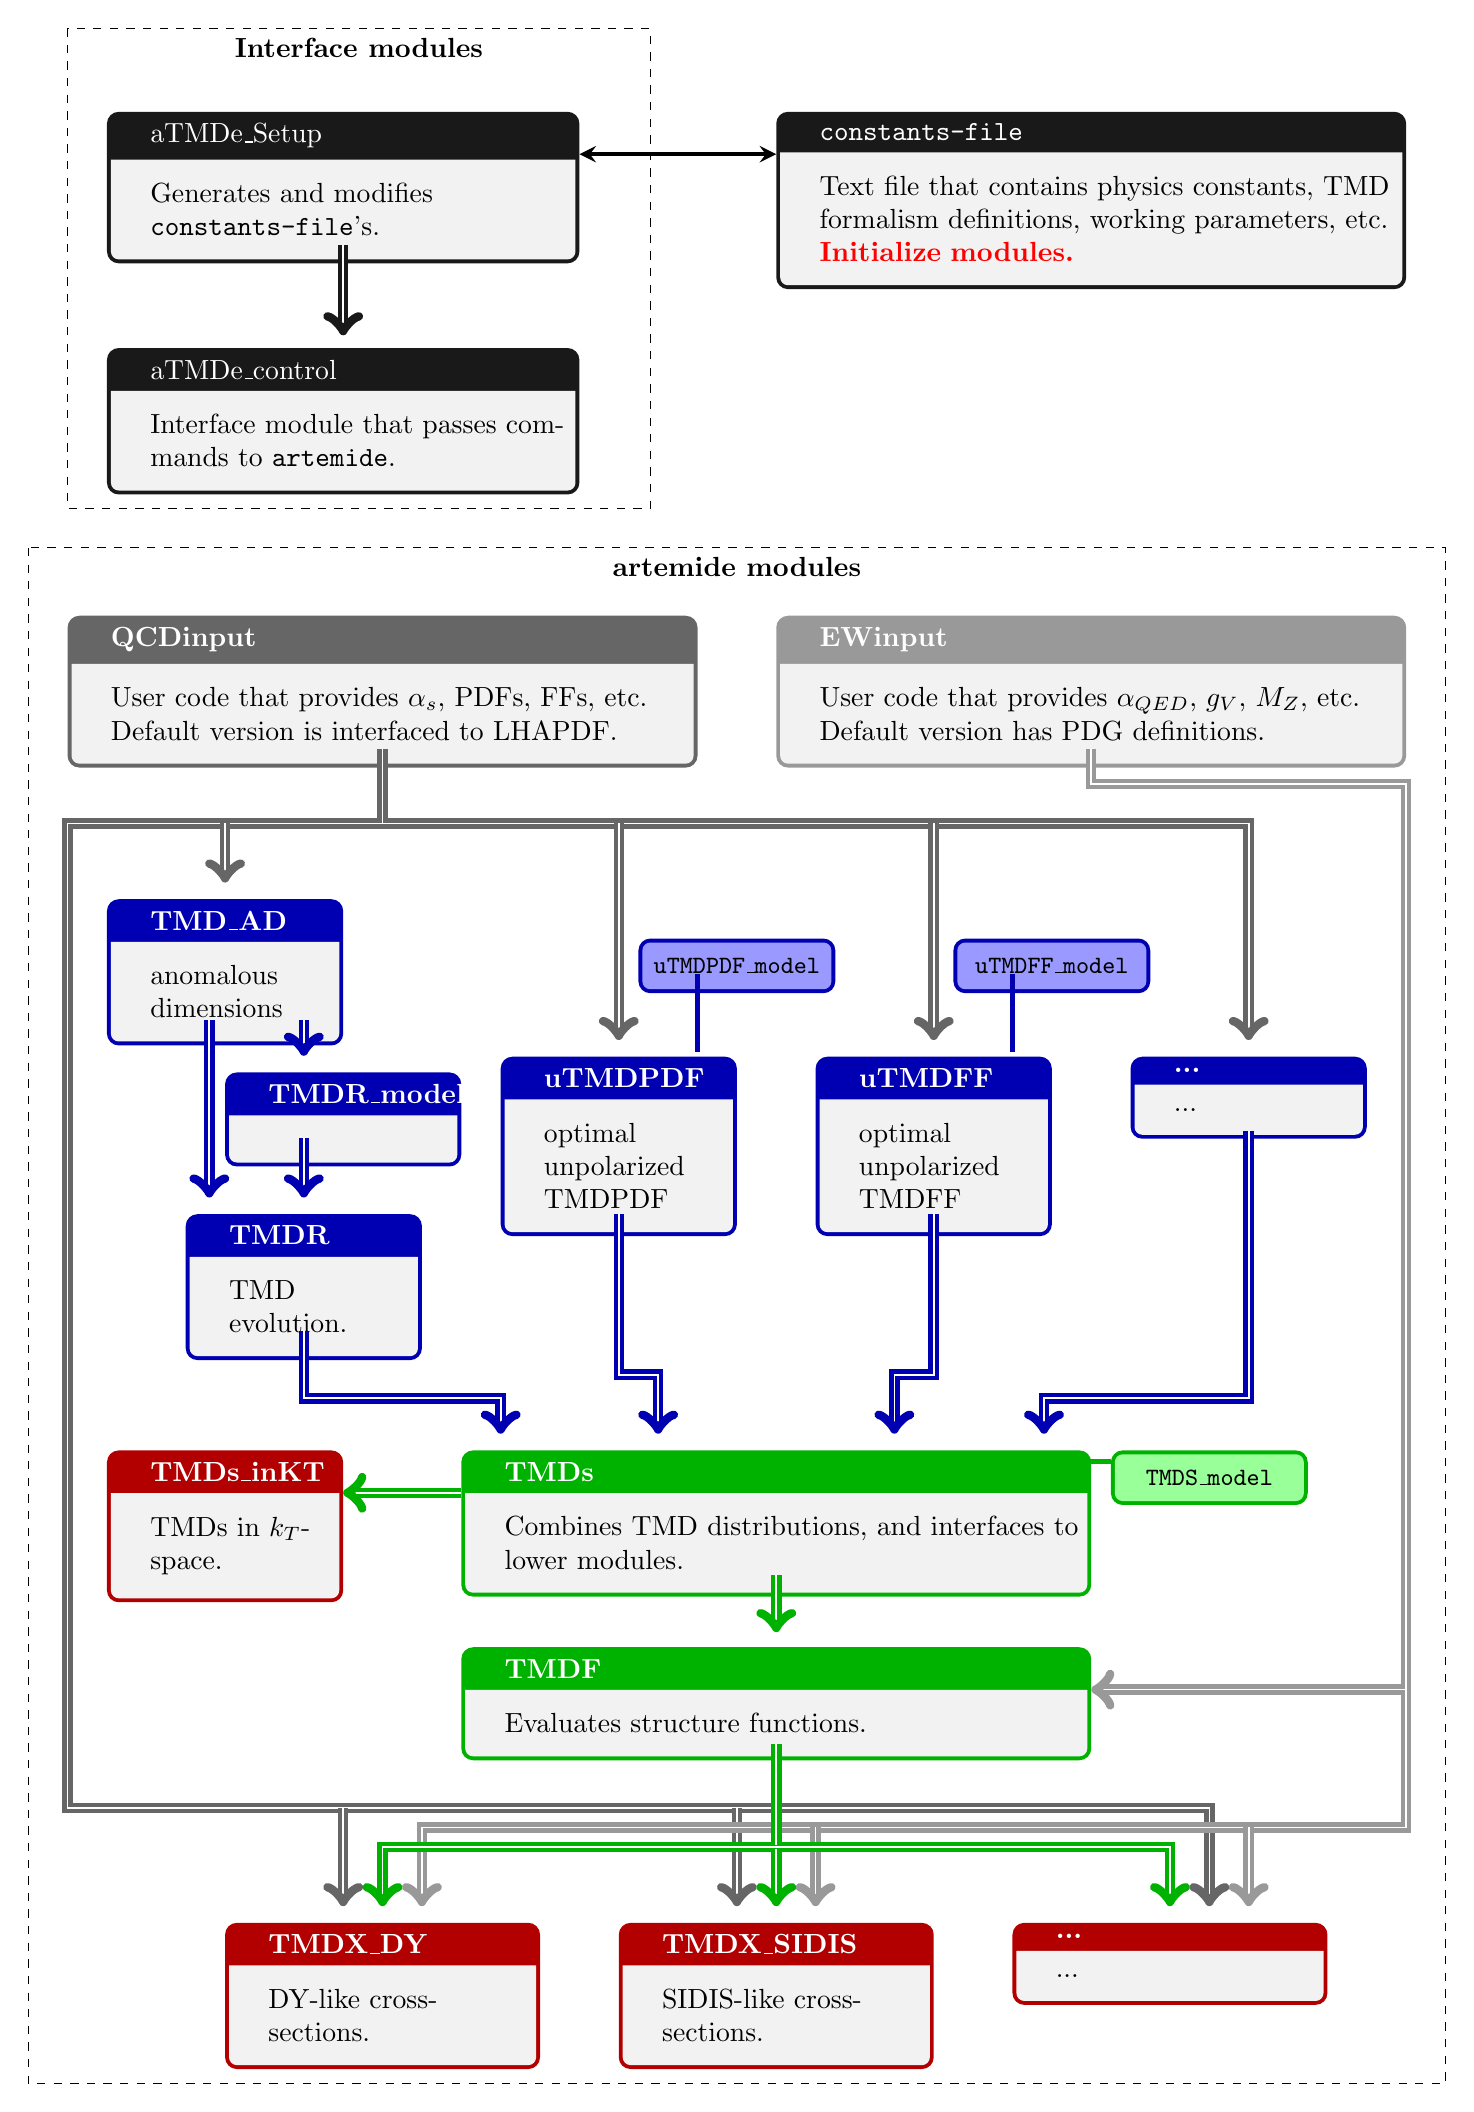
\begin{tikzpicture}

\draw[black,dashed] (-2,16.6) rectangle (5.4,10.5);
\node[below] at (1.7,16.6) {\textbf{Interface modules}};

\node [text width=8cm,below] at (11,16) {
\begin{tcolorbox}[enhanced,title=\texttt{constants-file},colframe=black!90!white,rightupper=0mm]
Text file that contains physics constants, TMD formalism definitions, working parameters, etc.
\\
\red{\textbf{Initialize modules.}}
\end{tcolorbox}};

\node [text width=6cm,below] at (1.5,16) {
\begin{tcolorbox}[enhanced,title=aTMDe\_Setup,colframe=black!90!white,rightupper=0mm]
Generates and modifies \texttt{constants-file}'s.
\end{tcolorbox}};

\node [text width=6cm,below] at (1.5,13) {
\begin{tcolorbox}[enhanced,title=aTMDe\_control,colframe=black!90!white,rightupper=0mm]
Interface module that passes commands to \texttt{artemide}. 
\end{tcolorbox}};

\draw[stealth-stealth,black,ultra thick] (4.5,15)--(7.,15);
\draw[->,white!10!black,ultra thick,double] (1.5,13.85)--(1.5,12.7);
%%%%%%%%%%%%%%%%%%%%%%%%%%%%%%%%%%%%%%%%%%%%%%%%%%%%%%%%%%%%%%%%%%%%%%%%%%%%%%%%%%%%%%%%%%%%%%%%%%%%%%%%%%%%%%%%
\draw[black,dashed] (-2.5,10) rectangle (15.5,-9.5);
\node[below] at (6.5,10) {\textbf{artemide modules}};

\node [text width=8cm,below] at (2,9.6) {
\begin{tcolorbox}[enhanced,title=QCDinput,colframe=black!60!white,fonttitle=\bfseries,
rightupper=0mm]
User code that provides $\alpha_s$, PDFs, FFs, etc.

Default version is interfaced to LHAPDF.
\end{tcolorbox}};

\node [text width=8cm,below] at (11,9.6) {
\begin{tcolorbox}[enhanced,title=EWinput,colframe=black!40!white,fonttitle=\bfseries,
rightupper=0mm]
User code that provides $\alpha_{QED}$, $g_V$, $M_Z$, etc.

Default version has PDG definitions.
\end{tcolorbox}};

\node [text width=3cm,below] at (0,6.) {
\begin{tcolorbox}[enhanced,title=TMD\_AD,colframe=blue!70!black,fonttitle=\bfseries,
rightupper=0mm]
anomalous \\ dimensions
\end{tcolorbox}};

\node [text width=3cm,below] at (1.5,3.8) {
\begin{tcolorbox}[enhanced,title=TMDR\_model,colframe=blue!70!black,fonttitle=\bfseries,
rightupper=0mm]
\end{tcolorbox}};

\node [text width=3cm,below] at (1,2) {
\begin{tcolorbox}[enhanced,title=TMDR,colframe=blue!70!black,fonttitle=\bfseries,
rightupper=0mm]
TMD \\ evolution.
\end{tcolorbox}};
\draw[->,blue!70!black,ultra thick,double] (-0.2,4.) -- (-0.2,1.75);
\draw[->,blue!70!black,ultra thick,double] (1,4.) -- (1,3.55);
\draw[->,blue!70!black,ultra thick,double] (1,2.5) -- (1,1.75);

\node [text width=3cm,below] at (5,4) {
\begin{tcolorbox}[enhanced,title=uTMDPDF,colframe=blue!70!black,fonttitle=\bfseries,
rightupper=0mm]
optimal
\\
unpolarized TMDPDF
\end{tcolorbox}};

\node [text width=2.5cm,below] at (6.5,5.5) {
\begin{tcolorbox}[enhanced,colframe=blue!70!black,fonttitle=\bfseries,
rightupper=0mm,colback=blue!40!white,left=0mm,top=1mm,bottom=1mm]
\center{\small \texttt{uTMDPDF{\_}model}}
\end{tcolorbox}};
\draw[blue!70!black,ultra thick] (6.,4.59)--(6.,3.6);

\node [text width=3cm,below] at (9,4) {
\begin{tcolorbox}[enhanced,title=uTMDFF,colframe=blue!70!black,fonttitle=\bfseries,
rightupper=0mm]
optimal
\\
unpolarized TMDFF
\end{tcolorbox}};

\node [text width=2.5cm,below] at (10.5,5.5) {
\begin{tcolorbox}[enhanced,colframe=blue!70!black,fonttitle=\bfseries,
rightupper=0mm,colback=blue!40!white,left=0mm,top=1mm,bottom=1mm]
\center{\small \texttt{uTMDFF{\_}model}}
\end{tcolorbox}};
\draw[blue!70!black,ultra thick] (10.,4.59)--(10.,3.6);

\node [text width=3cm,below] at (13,4) {
\begin{tcolorbox}[enhanced,title=...,colframe=blue!70!black,fonttitle=\bfseries,
rightupper=0mm]
...
\end{tcolorbox}};


\draw[<->,black!60!white,ultra thick,double] (12.5,-7.25)--(12.5,-6)--(-2,-6)--(-2,6.5) -- (13,6.5) -- (13,3.75);
\draw[->,black!60!white,ultra thick,double] (6.5,-6)--(6.5,-7.25);
\draw[->,black!60!white,ultra thick,double] (1.5,-6)--(1.5,-7.25);
\draw[black!60!white,ultra thick,double] (2,7.45) -- (2,6.5);
\draw[->,black!60!white,ultra thick,double] (9,6.5) -- (9,3.75);
\draw[->,black!60!white,ultra thick,double] (5,6.5) -- (5,3.75);
\draw[->,black!60!white,ultra thick,double] (0,6.5) -- (0,5.75);

\draw[->,black!40!white,ultra thick,double] (11,7.45)--(11,7.0)--(15,7.0)--(15,-4.5)--(11,-4.5);
\draw[->,black!40!white,ultra thick,double] (15,-4.5)--(15,-6.25)--(2.5,-6.25)--(2.5,-7.25);
\draw[->,black!40!white,ultra thick,double] (7.5,-6.25)--(7.5,-7.25);
\draw[->,black!40!white,ultra thick,double] (13,-6.25)--(13,-7.25);

\node [text width=8cm,below] at (7,-1) {
\begin{tcolorbox}[enhanced,title=TMDs,colframe=green!70!black,fonttitle=\bfseries,
rightupper=0mm]
Combines TMD distributions, and interfaces to lower modules.
\end{tcolorbox}};

\draw[->,green!70!black,ultra thick,double] (3,-2) -- (1.5,-2);
\node [text width=3cm,below] at (0,-1) {
\begin{tcolorbox}[enhanced,title=TMDs\_inKT,colframe=red!70!black,fonttitle=\bfseries,
rightupper=0mm]
TMDs in $k_T$-space.
\end{tcolorbox}};

\node [text width=2.5cm,below] at (12.5,-1) {
\begin{tcolorbox}[enhanced,colframe=green!70!black,fonttitle=\bfseries,
rightupper=0mm,colback=green!40!white,left=0mm,top=1mm,bottom=1mm]
\center{\small \texttt{TMDS{\_}model}}
\end{tcolorbox}};
\draw[green!70!black,ultra thick] (10.,-1.6)--(11.25,-1.6);

\draw[->,blue!70!black,ultra thick,double] (1,0.05) -- (1,-.8)-- (3.5,-.8)-- (3.5,-1.25);
\draw[->,blue!70!black,ultra thick,double] (5,1.54) -- (5,-0.5)-- (5.5,-0.5)-- (5.5,-1.25);
\draw[->,blue!70!black,ultra thick,double] (9,1.54) -- (9,-0.5)-- (8.5,-0.5)-- (8.5,-1.25);
\draw[->,blue!70!black,ultra thick,double] (13,2.6) -- (13,-.8)-- (10.4,-.8)-- (10.4,-1.25);

\node [text width=8cm,below] at (7,-3.5) {
\begin{tcolorbox}[enhanced,title=TMDF,colframe=green!70!black,fonttitle=\bfseries,
rightupper=0mm]
Evaluates structure functions.
\end{tcolorbox}};

\draw[->,green!70!black,ultra thick,double] (7,-3.05) -- (7,-3.77);

\node [text width=4cm,below] at (2,-7) {
\begin{tcolorbox}[enhanced,title=TMDX{\_}DY,colframe=red!70!black,fonttitle=\bfseries,
rightupper=0mm]
DY-like cross-sections.
\end{tcolorbox}};

\node [text width=4cm,below] at (7,-7) {
\begin{tcolorbox}[enhanced,title=TMDX{\_}SIDIS,colframe=red!70!black,fonttitle=\bfseries,
rightupper=0mm]
SIDIS-like cross-sections.
\end{tcolorbox}};

\node [text width=4cm,below] at (12,-7) {
\begin{tcolorbox}[enhanced,title=...,colframe=red!70!black,fonttitle=\bfseries,
rightupper=0mm]
...
\end{tcolorbox}};

\draw[<->,green!70!black,ultra thick,double] (2,-7.25) -- (2,-6.5) -- (12,-6.5) -- (12,-7.25);
\draw[green!70!black,ultra thick,double] (7,-6.47) -- (7,-5.19);
\draw[->,green!70!black,ultra thick,double] (7,-6.52) -- (7,-7.25);

\end{tikzpicture}
}
\end{center}
\caption{\label{fig:dependencies}{\Large Modules of \texttt{artemide}: purpose and dependencies}}
\end{figure}

\subsection{Organization of TMD factorized cross-section and its implementation in \texttt{artemide}}

The ultimate goal of the \texttt{artemide} is to evaluate the observables in the TMD factorization framework, such as cross-section, asymmetries, etc. The general structure of the TMD factorized \textit{fully differential} cross-section  is
\begin{eqnarray}
\frac{d\sigma}{dX}=
d\sigma(q_T)=prefactor~\times F,
\end{eqnarray}
where 
$prefactor$ a process-dependent and experiment-dependent prefactor, and $F$ is the reduced structure function. Example, for the photon induced Drell-Yan process one has for $d\sigma/dq_T$
\begin{eqnarray*}
prefactor&=&\frac{4\pi}{9sQ^2}|C_V(Q,\mu_H)|^2 \mathcal{P}(\text{cuts}),
\\
F&=&\int \frac{bdb}{2}J_0(bq_T)\sum_{f}|e_f|^2F_{f}(x_A,b;\mu_H,\zeta_A)F_{\bar f}(x_B,b;\mu_H,\zeta_B),
\end{eqnarray*}
where $\mathcal{P}(\text{cuts})$ is the weighting factor for fiducial cuts. For specific expression we refer in corresponding sections of this text. The structure function $F$ is generally defined as
\begin{eqnarray}
F(q_T,x_1,x_2;\mu,\zeta_1,\zeta_2)=\int \frac{b db}{2}b^{n}J_n(b q_T)\sum_{ff'} z_{ff'} F^f_1(x_1,b;\mu,\zeta_1)F^{f'}_2(x_2,b;\mu,\zeta_2),
\end{eqnarray}
where $F_{1,2}$ are TMD distributions (of any origin and polarization), $z_{ff'}$ is the process dependent flavor mixing factor. The number $n$ is also process dependent, e.g. for unpolarized observables it is $n=0$, while for SSA's it is $n=1$. Evaluation structure functions $F$ is performed in the module \texttt{TMDF}. The evaluation of cross-sections is performed in the modules \texttt{TMDX}. The TMD distributions are evaluated by the module \texttt{TMDs} and related submodules.

\begin{tcolorbox}
In this way, the computation of TMD-factorized cross-section can be naturally split into ordered parts. Each part is evaluated in corresponding module of \texttt{artemide}. See example, of evaluation scheme in fig.\ref{fig:order_of_evaluation}.
\end{tcolorbox}

\subsection{User defined functions and options}

\begin{tcolorbox}
The \texttt{artemide} package has been created such that it allows to control \textbf{each aspect} of TMD factorization theorem. The TMD factorization has a large number of free, and ``almost-free'' parameters. It is a generally difficult task to provide a convenient interface for all these inputs. I do my best to make the interface convenient; however, some parts (e.g., setup of $f_{NP}$) could not be simpler (at least within FORTRAN). Also, take care that \texttt{artemide} is evolving, and I try to keep back compatibility, but it is not the main option.
\end{tcolorbox}

\begin{tcolorbox}
Starting from ver.2.0, \texttt{artemide} uses the text initialization file, which contains all required information on static parameters for a given setup. Throughout the text I call this file \texttt{constants-file}.
\end{tcolorbox}

The user has to provide (or \textbf{use the default values}) the set of parameters, that control various aspects of evaluation. It includes PDF sets, $f_{NP}$, perturbative scales, parameters of numerics, non-QCD inputs, etc.  There are three input sources for statical parameters.

\begin{itemize}
\item[~] \textbf{General parameters:} These are working parameters of \texttt{artemide}, such as amount of output, tolerance of integration routines, number of NP parameters, type of used evolution, griding parameters, triggering of particular contributions, etc. There are many of them, and typically they are unchanged. These are set in \texttt{constants-file}. \textbf{Changes do not require recompilation.}
\item[~] \textbf{External physics input:} It includes the definition of $\alpha_s$, collinear PDFs, and other distributions. Twist-2 distributions are taken from LHAPDF \cite{Buckley:2014ana}, with routines defined in \text{QCDinput} module. For non-QCD parameters, e.g. $\alpha_{QED}$, SM parameters, there is a module \texttt{EWinput}. These are set in \texttt{constants-file}. \textbf{Changes do not require recompilation.}
\item[~] \textbf{NP model:} The NP model consists in NP profiles of TMD distributions, NP model for large-b evolution, selection of scales $\mu$, etc. These parameter and functions enter nearly each low level module. The code for corresponding functions is provided by user, in appropriate files, which are collected in the subdirectory \texttt{src/Model}. The name of files are shown on diagram in colored blobs adjusted to the related module. \red{\textbf{Changes require recompilation.}}
\end{itemize}

\textbf{Comments:}
\begin{itemize}
\item \textbf{IMPORTANT:} Each module is initialized individually via \texttt{constants-file}. So, each module can be used independently on the full package, given proper section of \texttt{constants-file} and submodules (see diagram). However, unless you understand what is going on, it is recommended to use \texttt{aTMDe\_setup} module for  creation of \texttt{constant-file}, and \texttt{aTMDe\_control} module for proper control, initialization and operations of sub-modules.
\item \texttt{constants-file} can be saved and used in future to reproduce setup. I try to keep compatibility between these files.
\item \texttt{constants-file} is created and modified within \texttt{aTMDe\_setup} module. It could be also modified manually.
\item NP functions are typically defined with a number of numeric parameters. The value of these parameters could be changed without restart (or recompilation) of the \texttt{artemide} by appropriate command. E.g. (\texttt{call TMDs{\_}SetNPParameters(lambda)}) on the level of \texttt{TMDs} module. See sections of corresponding modules.
\item The number of parameters in the model for each module is set in \texttt{constants-file}.
\item The directory \texttt{/Model} together with \texttt{constants-file} are convenient to keep as they are. They contain full information about particular evaluation, and thus results can be always reproduced (at least within the same version of \texttt{artemide}). I provide results of our extraction as such directories. 
\item Before ver.2.0, the interface was different and chaotic.
\end{itemize}

\subsection{Installation}

Download and unpack \texttt{artemide}. The actual code is in the /src. Check the \texttt{makefile}. \red{\textbf{You must provide options \texttt{FC} and \texttt{FOPT}, which are defined in the top of it.}} \texttt{FC} is the FORTRAN compiler, \texttt{FOPT} is additional options for compiler (e.g. linking to LHAPDF library).

There is no actual installation procedure, there is just compilation. If model, inputs, etc, are set correctly (typical problem is linking to LHAPDF, be sure that it is installed correctly), then \texttt{make} compiles the library. The result are object files (\texttt{*.o}) (which are collected in \texttt{/obj}) and module files (\texttt{*.mod}) (which are collected in \texttt{/mod}). 

The test of current compilation could be performed by \texttt{make test}. It compiles program \texttt{test.f90} from /Prog and run it (default test uses \texttt{NPDF31\_nnlo\_as\_0118} set from LHAPDF, check that it is present in your LHAPDF installation). Program \texttt{test} runs some elementary code with minimum input. Output is shown later

Next, do your code, \texttt{include} appropriate modules of \texttt{artemide}, and compile it together with object-files (do not forget to add proper references to module files \texttt{-I/mod}). It should work! Linking could be done automatically if you call for \texttt{make program TARGET=...}, where ... is the name of the file with the code.

%\lstset{style=DOS}
\begin{lstlisting}[{style=DOS}]
  artemide.control: initialization done.
 uTMDPDF: Grid is built  (  250 x  750)  calc.time=  0.53s. 
 Calculating some values for cross-section one-by-one (DY around Z-boson peak, ATLAS 8TeV kinematics)
 ptMin 	--	ptMax		xSec
   1.0000000000000000      --   3.0000000000000000        48.499041273610260     
   3.0000000000000000      --   5.0000000000000000        57.189916866533792     
   5.0000000000000000      --   7.0000000000000000        49.321931214709110     
  
 Now the same by list
 It must be faster since you use OPENMP
 result:   48.499041273610260        57.189916866533792        49.321931214709110     
 -----------------------------------------------------------------------------------------------
 The programm evaluation took   8.8279999999999994      sec. (CPU time)
 The programm evaluation took   6.1287177319172770      sec. (wallclock time)
   
 If you do not like so many terminal messages check the parameter outputlevel in constants file.
 Not forget to cite artemide [1706.01473]
 -----------------------------------------------------------------------------------------------


\end{lstlisting}

\subsection{Python interface: \texttt{harpy}}

For simplicity of data analysis the \texttt{artemide} has a python interface, called \texttt{harpy} (linking is made by f2py library). It is not possible to interfacing the \texttt{artemide} directly  to python since \texttt{artemide} is made on fortran95. \texttt{Artemide} uses some features of Fortran95, such as interfaces, and indirect list declarations, which are alien to python. Also I have not found any convenient way to include several dependent Fortran modules in f2py (if you have suggestion just tell me). Therefore, I made a wrap module \texttt{harpy.f90} that call some useful functions from \texttt{artemide} with simple declarations. It contains limited set of functions useful for phenomenology, and definitely cannot replace the FORTRAN interface for deep studies.

The compilation of \texttt{harpy} is slightly more complicated.

\begin{enumerate}
\item In the makefile check the variable \texttt{Fpath} (in the top part of the file). Put-in the full path for fortran compiler. It is needed by f2py.
\item (optional, does not work on Mac (?)) Run \texttt{make harpy-signature} . This will create an interface file (\texttt{artemide.pyf} for all functions in the \texttt{harpy.f90}. This file is already provided in the distribution, so if you did not change \texttt{harpy.f90}, you better skip this step. For some reason, it does not work on Mac.
\item Run \texttt{make harpy}. It compiles \texttt{harpy.f90} with interface \texttt{artemide.pyf} linking to \texttt{artemide}. The result is \texttt{artemide.so}.
\end{enumerate}

All files are in /harpy. Link it to python and work. There is also extra python \texttt{harpy.py} which has several most important function.

\subsection{Constants file and version compatibility}

Constants files contains the list of work-flow parameters, such as physical constants, LHA grid names, numerical setup, etc. Each constants file has version number (does not coincide with the version of artemide). 

On the module initialization the constants file is read, parameter are setup. Thus, the version of constants file should be adjusted to version of artemide \textit{if you run modules separately}.

The workflow is deferent of the initialization of \texttt{artemide} is made by the \texttt{artemide\_control}. In this case, the \texttt{artemide} creates a copy of the initial constants-file (\texttt{aTMDe\_temporary}), and (in the case the versions do not match) fill the absent options by default parameter. After it the lower-level modules are initialized by \texttt{aTMDe\_temporary}. Naturally, in this case the versions should match (if not something is wrong with installation).

\begin{tcolorbox}
You can update the \texttt{constants-file} to an actual version by 
\\
\texttt{make update TARGET=...}
\\
where ... is the path to \texttt{constants-file} to be updated. The updated version will have all content of the original file, + new options setup by default setting.
\end{tcolorbox}

\begin{figure}
\begin{center}
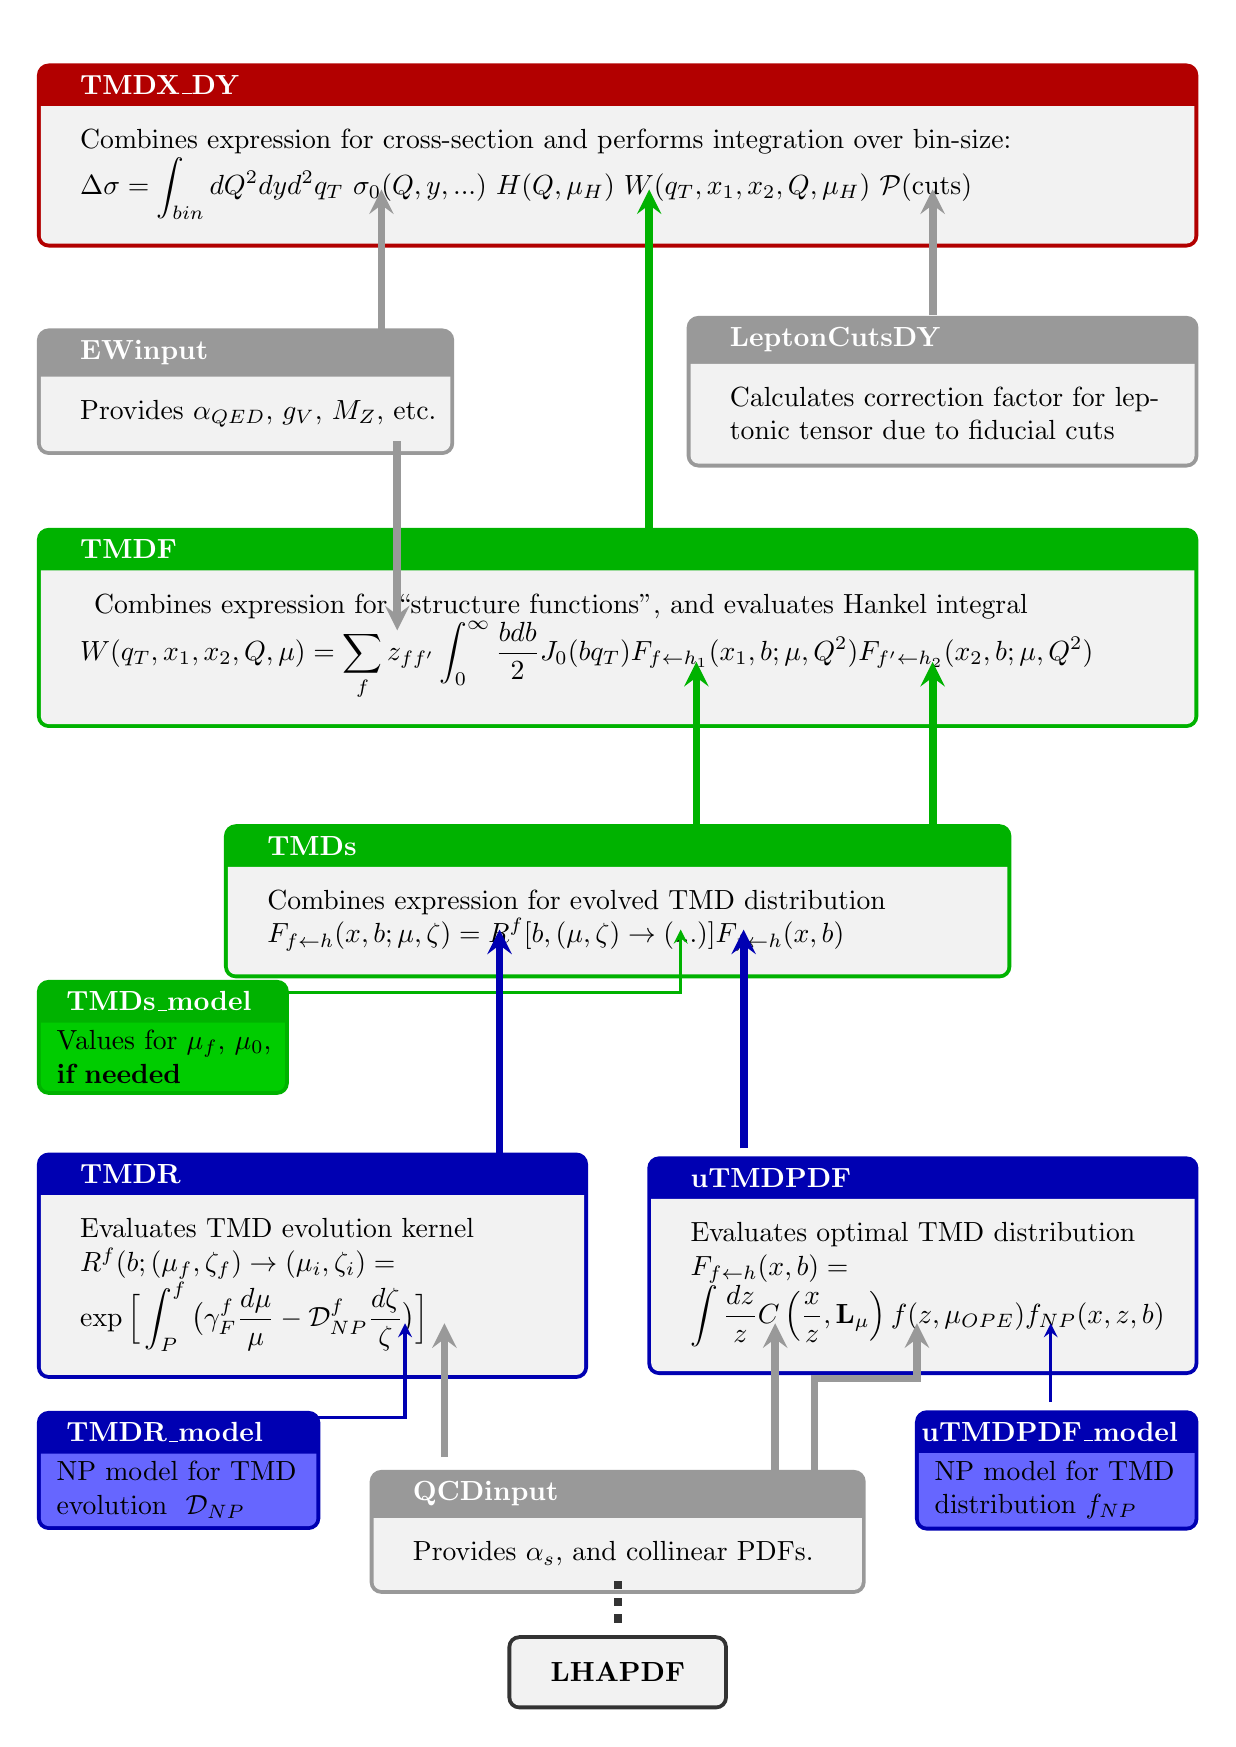
\begin{tikzpicture}
%\draw[step=1cm] (0,0) to[grid with coordinates] (16,25);

\node [text width=14.75cm,right] at (0.5,24) {
\begin{tcolorbox}[enhanced,title=TMDX\_DY,colframe=red!70!black,fonttitle=\bfseries,
rightupper=0mm]
Combines expression for cross-section and performs integration over bin-size:
\\
 $\Ds \Delta \sigma = \int_{bin}dQ^2 dy d^2q_T ~\sigma_0(Q,y,...) ~ H(Q,\mu_H)~ W(q_T,x_1,x_2,Q,\mu_H)~\mathcal{P}(\text{cuts})$
\end{tcolorbox}};


\node [text width=5.3cm,right] at (0.5,21) {
\begin{tcolorbox}[enhanced,title=EWinput,colframe=black!40!white,fonttitle=\bfseries,
rightupper=0mm]
Provides $\alpha_{QED}$, $g_V$, $M_Z$, etc.
\end{tcolorbox}};
\draw[-stealth,black!40!white,line width=2.8pt] (5,21.5) -- (5,23.4);

\node [text width=6.5cm,left] at (15.5,21) {
\begin{tcolorbox}[enhanced,title=LeptonCutsDY,colframe=black!40!white,fonttitle=\bfseries,
rightupper=0mm]
Calculates correction factor for leptonic tensor due to fiducial cuts
\end{tcolorbox}};
\draw[-stealth,black!40!white,line width=2.8pt] (12,21.8) -- (12,23.4);


\node [text width=14.75cm,right] at (0.5,18) {
\begin{tcolorbox}[enhanced,title=TMDF,colframe=green!70!black,fonttitle=\bfseries,
rightupper=0mm]
~\,Combines expression for ``structure functions'', and evaluates Hankel integral
\\
$\Ds W(q_T,x_1,x_2,Q,\mu)=\sum_f z_{ff'} \int_0^\infty \frac{bdb}{2}J_0(b q_T)F_{f\ot h_1}(x_1,b;\mu,Q^2)F_{f'\ot h_2}(x_2,b;\mu,Q^2)$
\end{tcolorbox}};
\draw[-stealth,black!40!white,line width=2.8pt] (5.2,20.2) -- (5.2,17.8);
\draw[-stealth,green!70!black,line width=2.8pt] (8.4,19) -- (8.4,23.4);

\node [text width=10cm,below] at (8,15.8) {
\begin{tcolorbox}[enhanced,title=TMDs,colframe=green!70!black,fonttitle=\bfseries,
rightupper=0mm]
Combines expression for evolved TMD distribution
\\
$\Ds F_{f\ot h}(x,b;\mu,\zeta)=R^f[b,(\mu,\zeta)\to(...)]F_{f\ot h}(x,b)$
\end{tcolorbox}};
\draw[-stealth,green!70!black,line width=2.8pt] (9,15.2) -- (9,17.4);
\draw[-stealth,green!70!black,line width=2.8pt] (12,15.2) -- (12,17.4);

\node [text width=3.2cm,right] at (0.5,12.8) {
\begin{tcolorbox}[enhanced,title=$\!\!\!$TMDs\_model,colframe=green!70!black,fonttitle=\bfseries,
rightupper=0mm,top=0mm,bottom=0mm,leftupper=1mm,colback=green!80!black]
Values for $\mu_f$, $\mu_0$,
~~~\textbf{if needed}
\end{tcolorbox}};
\draw[-stealth,green!70!black,line width=1.2pt] (3.5,13.2) --(8.8,13.2)-- (8.8,14);

\node [text width=7cm,right] at (0.5,9.9) {
\begin{tcolorbox}[enhanced,title=TMDR,colframe=blue!70!black,fonttitle=\bfseries,
rightupper=0mm]
Evaluates TMD evolution kernel
\\
$R^f(b;(\mu_f,\zeta_f)\to(\mu_i,\zeta_i)=$
\\ $\Ds~\qquad\quad \exp\Big[\int^f_P \big(\gamma^f_F\frac{d\mu}{\mu}-\mathcal{D}^f_{NP}\frac{d\zeta}{\zeta}\big)\Big] $
\end{tcolorbox}};
\draw[-stealth,blue!70!black,line width=2.8pt] (6.5,11) -- (6.5,14.);

\node [text width=7cm,left] at (15.5,9.9) {
\begin{tcolorbox}[enhanced,title=uTMDPDF,colframe=blue!70!black,fonttitle=\bfseries,
rightupper=0mm]
Evaluates optimal TMD distribution
\\
$\Ds F_{f\ot h}(x,b)=$\\
$\Ds\int \frac{dz}{z}C\(\frac{x}{z},\mathbf{L}_\mu\) f(z,\mu_{OPE}) f_{NP}(x,z,b) $
\end{tcolorbox}};
\draw[-stealth,blue!70!black,line width=2.8pt] (9.6,11.22) -- (9.6,14.);


\node [text width=3.6cm,right] at (0.5,7.3) {
\begin{tcolorbox}[enhanced,title=$\!\!\!$TMDR\_model,colframe=blue!70!black,fonttitle=\bfseries,
rightupper=0mm,top=0mm,bottom=0mm,leftupper=1mm,colback=blue!60!white]
NP model for TMD evolution $~\mathcal{D}_{NP}$
\end{tcolorbox}};
\draw[-stealth,blue!70!black,line width=1.2pt] (3.5,7.8) --(5.3,7.8)-- (5.3,9);

\node [text width=3.6cm,left] at (15.5,7.3) {
\begin{tcolorbox}[enhanced,title=$\!\!\!\!\!\!\!\!$uTMDPDF\_model,colframe=blue!70!black,fonttitle=\bfseries,
rightupper=0mm,top=0mm,bottom=0mm,leftupper=1mm,colback=blue!60!white]
NP model for TMD distribution $f_{NP}$
\end{tcolorbox}};
\draw[-stealth,blue!70!black,line width=1.2pt] (13.5,8.) --(13.5,9.);

\node [text width=6.3cm,below] at (8,7.6) {
\begin{tcolorbox}[enhanced,title=QCDinput,colframe=black!40!white,fonttitle=\bfseries,
rightupper=0mm]
Provides $\alpha_{s}$, and collinear PDFs.
\end{tcolorbox}};
\draw[-stealth,black!40!white,line width=2.8pt] (5.8,7.3) -- (5.8,9);
\draw[-stealth,black!40!white,line width=2.8pt] (10,7) -- (10,9);
\draw[-stealth,black!40!white,line width=2.8pt] (10.5,7) -- (10.5,8.3)-- (11.8,8.3)-- (11.8,9);

\node [text width=2.8cm,below] at (8,5.5) {
\begin{tcolorbox}[enhanced,colframe=black!80!white,fonttitle=\bfseries,
rightupper=0mm]
\textbf{LHAPDF}
\end{tcolorbox}};

\draw[black!80!white,line width=2.8pt,dashed] (8,5.2) -- (8,5.8);

\end{tikzpicture}
\end{center}
\caption{\label{fig:order_of_evaluation} {\Large Evaluation of DY cross-section by \texttt{artemide}}}
\end{figure}

\newpage

\section{Theory}

\begin{center}
\red{\textbf{This section is under construction.}}
\end{center}

In this section, the details of theoretical input coded in \texttt{artemide} is given. This section does not pretend to be a comprehensive review of TMD factorization. Only superficial details and references to particular realizations are given. For detailed and accurate description of the theory see specialized literature.

\subsection{Definition of TMD distributions}

\red{TO BE WRITTEN}. In this section, there will be operator definition of TMD distributions, and details on way the perturbative matching and NP-medeling is realized in \texttt{artemide}.

\begin{eqnarray}
F_f(x,b)=\int_x^1 \frac{dz}{z}C_{f\ot f'}(z,b^*,c_4\mu_\text{OPE})f_{f'}(\frac{z}{x},c_4\mu_\text{OPE})f^f_{NP}(x,z,b,\{\lambda\}),
\end{eqnarray}
where $f_f(x,\mu)$ is PDF of flavor $f$, $C$ is the coefficient function in $\zeta$-prescription, $f_{NP}$ is the non-perturbative function. The variable $c_4$ is used to test the scale variation sensitivity of the TMD PDF. The NNLO coefficient functions used in the module were evaluated in \cite{Echevarria:2016scs} (please, cite it if use).


\red{PLAN TO ADD}
\begin{itemize}
\item Definition of TMD distributions, operators, Lorenz structures, coordinate and momentum space. 
\item Perturbative matching, and $\zeta$-prescription
\item NP-modeling
\end{itemize}


\subsection{Evolution of TMD distributions}

The detailed theory is given in the article \cite{Scimemi:2018xaf}. The NLO rapidity anomalous dimension has been evaluated in \cite{Echevarria:2015byo}. The NNLO rapidity anomalous dimension has been evaluated in \cite{Vladimirov:2016dll,Vladimirov:2017ksc}.

The evolution of TMD distribution of any kind is given by the following pair of equations
\begin{eqnarray}\label{def:TMD_ev_UV}
\mu^2 \frac{d}{d\mu^2} F_{f\ot h}(x,b;\mu,\zeta)&=&\frac{\gamma^f_F(\mu,\zeta)}{2}F_{f\ot h}(x,b;\mu,\zeta),
\\\label{def:TMD_ev_RAP}
\zeta\frac{d}{d\zeta}F_{f \ot h}(x,b;\mu,\zeta)&=& -\mathcal{D}^f(\mu,b)F_{f\ot h}(x,b;\mu,\zeta),
\end{eqnarray}
where $F_{f\ot h}$ is the TMD distribution (TMDPDF or TMDFF) of the parton $f$ in hadron $h$. The function $\gamma_F(\mu,\zeta)$ is called the TMD anomalous dimension and contains both single and double logarithms. The function $\mathcal{D}(\mu,b)$ is called the rapidity anomalous dimension. TMD and rapidity anomalous dimensions have not unified notation in the literature, for comparison of notation see table I in ref.\cite{Scimemi:2018xaf}. The only important quantum number for TMDs is the color representation the initiating parton, which is tied to the parton flavor, namely, quark (fundamental representation) or gluon (adjoint representation). However,  as the TMD evolution does not mix the flavors and  for simplicity of  notation, we omit the flavor index $f$ in this section, unless it is important. 

The uniqueness of solution for the coupled system (\ref{def:TMD_ev_UV})-(\ref{def:TMD_ev_RAP}) is guaranteed by \textit{the integrability condition}
\begin{eqnarray}\label{th:consitency}
\zeta \frac{d}{d\zeta}\gamma_F(\mu,\zeta)=-\mu \frac{d}{d\mu}\mathcal{D}(\mu,b),
\end{eqnarray} 
The mutual dependence can be worked out  explicitlydue to the fact that the ultraviolet divergences of the TMD operator partially overlap with the rapidity divergences, (see e.g.\cite{Collins:2011zzd,Vladimirov:2017ksc}), 
\begin{eqnarray}\label{th:dGammaF=G}
\zeta \frac{d}{d\zeta}\gamma_F(\mu,\zeta)=-\Gamma(\mu),
\\\label{th:dDD=G}
\mu \frac{d}{d\mu}\mathcal{D}(\mu,b)=\Gamma(\mu),
\end{eqnarray}
where $\Gamma$ is the (light-like) cusp anomalous dimension. The equation (\ref{th:dGammaF=G}) entirely fixes the logarithm dependence of the TMD anomalous dimension, which reads
\begin{eqnarray}\label{th:gammaV}
\gamma_F(\mu,\zeta)=\Gamma(\mu) \ln\(\frac{\mu^2}{\zeta}\)-\gamma_V(\mu).
\end{eqnarray}
The anomalous dimension $\gamma_V$ refers to the finite part of the renormalization of the vector form factor. In contrast, the equation (\ref{th:dDD=G}) cannot fix the logarithmic part of $\mathcal{D}$ entirely, but only order by order in  perturbation theory, because the parameter $\mu$ is also responsible for the running of the coupling constant.

The solution of eq.~(\ref{def:TMD_ev_UV})-(\ref{def:TMD_ev_RAP})  can be written as
\begin{eqnarray}\label{th:TMD_evol}
F(x,b;\mu_f,\zeta_f)=R[b;(\mu_f,\zeta_f)\to (\mu_i,\zeta_i)]F(x,b;\mu_i,\zeta_i),
\end{eqnarray}
where $R$ is the TMD evolution factor. The general form of the evolution factor is
\begin{eqnarray}\label{th:TMD_R}
R[b;(\mu_f,\zeta_f)\to (\mu_i,\zeta_i)]=\exp\[\int_P \(\gamma_F(\mu,\zeta)\frac{d\mu}{\mu} -\mathcal{D}(\mu,b)\frac{d\zeta}{\zeta}\)\] ,
\end{eqnarray}
where $(\mu_f,\zeta_f)$ and $(\mu_i,\zeta_i)$ refer respectively to a final  and initial set of scales. Here, the $\int_P$ denotes the line integral along the path $P$ in the $(\mu,\zeta)$-plane from the point $(\mu_f,\zeta_f)$ to the point $(\mu_i,\zeta_i)$. The integration can be done on an arbitrary path $P$, and the solution is independent on it, thanks to the integrability condition eq.~(\ref{th:consitency}). 

The TMD evolution factor $R$ obeys the transitivity relation
\begin{eqnarray}\label{th:transitivity}
R[b;(\mu_1,\zeta_1)\to (\mu_2,\zeta_2)]=R[b;(\mu_1,\zeta_1)\to (\mu_3,\zeta_3)]R[b;(\mu_3,\zeta_3)\to (\mu_2,\zeta_2)],
\end{eqnarray}
where $(\mu_3,\zeta_3)$ is arbitrary point in $(\mu,\zeta)$-plane and the  point inversion property
\begin{eqnarray}\label{th:inversion}
R[b;(\mu_1,\zeta_1)\to (\mu_2,\zeta_2)]=R^{-1}[b;(\mu_2,\zeta_2)\to (\mu_1,\zeta_1)].
\end{eqnarray}
These equations are the cornerstones of the evolution mechanism, since they allow an universal definition of the non-perturbative distributions and the comparison of different experiments. 

Different realizations of TMD evolution (if they are compatible with the factorization theorem) can be casted into selected of different paths of integration \red{ADD PICTURE}. All choices are equivalent, up to next-to-given order perturbative corrections, treatment of NP parts, and implementation of matching for TMD distributions. In \texttt{artemide} sevaral paths are presented, however, the matching of TMD distribution to collinear distributions is done in $\zeta$-prescription.

\subsubsection{Equipotential lines \& $\zeta$-prescription}

The $\zeta$-prescription is based on consideration of equipotential lines for evolution equations (\ref{def:TMD_ev_UV})-(\ref{def:TMD_ev_RAP}) (or lines of null-evolution, for description of evolution potential and its properties see \cite{Scimemi:2018xaf}). An equipotential line $\ell(b)=(\mu,\zeta)$ is determined by values of anomalous dimensions $\gamma_F$ and $\mathcal{D}$ at given $b$. The equation for line $\ell(b)$ can be written in the form $\zeta=\zeta(\mu,b)$. In this parameterization the for function $\zeta(\mu,b)$ is
\begin{eqnarray}\label{TMDR_th:3}
-\Gamma(\mu)\ln\(\frac{\zeta(\mu,b)}{\mu^2}\)-\gamma_V(\mu)=2\mathcal{D}(\mu,b)\frac{d\ln\zeta(\mu,b)}{d\ln\mu^2}.
\end{eqnarray}
Among set of equipotential lines there is a single special equipotential line, which passes thorough the saddle point of the evolution field. The saddle point $(\mu_{\text{saddle}},\zeta_{\text{saddle}})$ is defined by the equations
\begin{eqnarray}\label{TMDR_th:4}
\mathcal{D}(\mu_{\text{saddle}},b)=0,\qquad \gamma_V(\mu_{\text{saddle}},\zeta_{\text{saddle}})=0.
\end{eqnarray}
Note, that the value of $\mu_{\text{saddle}}$ depends on value of $b$, and on NP model for $\mathcal{D}$. In general it could be found only numerically. In typical models $\mu_{\text{saddle}}$ is decreasing monotonous function of $b$. At certain large values of $b$ it passes though the Landau pole, and its value could not be determined. This line we denote as
\begin{eqnarray}\label{TMDR_th:12}
\textbf{special equipotential line}=\zeta_\mu(b),\qquad (\mu_{\text{saddle}},\zeta_{\text{saddle}})\in \zeta_\mu(b).
\end{eqnarray}

By definition a TMD distribution is the same for all points of equipotential line. In particular it means that there is no dependence on variable $\mu$, since a variation of $\mu$ is compensated by appropriate variation in $\zeta(\mu)$. 

\textbf{Important note:} The presence of NP part in $\mathcal{D}$ makes determination of special line involved. We distinguish three ``realizations'' of the special line. The exact which is determined by equation (\ref{TMDR_th:3}) and boundary conditions (\ref{TMDR_th:12}) (its values can be calculated by function \texttt{zetaSL}). The perturbative realization where NP part is dropped (its values can be calculated by functions \texttt{zetaMUperp} and \texttt{zetaMUresum}). And user-defined which is given by user in \texttt{TMDR\_model.f90} file.

\subsubsection{Exact solution for evolution to special line}

There is a possibility to define the evolution to the optimal equipotential line in perturbation theory for any NP input, at any $b$. Instead of problematic variable $b$ one uses the function $\mathcal{D}(\mu,b)$ as a variable. With the ansatz $\zeta_\mu=\mu^2 \exp(-g(\mu,b))$ we rewrite equation (\ref{TMDR_th:3}) as
\begin{eqnarray}
2\mathcal{D}(\mu,b)\(1-\frac{dg(\mu,b)}{d\ln \mu^2}\)-\Gamma(\mu)g(\mu,b)+\gamma_V(\mu)=0.
\end{eqnarray}
or
\begin{eqnarray}\label{TMDR_th:16}
2\mathcal{D}\(1-\frac{\partial g(\mu,\mathcal{D})}{\partial \ln \mu^2}-\frac{\Gamma(\mu)}{2}g'(\mu,\mathcal{D})\)-\Gamma(\mu)g(\mu,\mathcal{D})+\gamma_V(\mu)=0,
\end{eqnarray}
where $g'=d g/d\mathcal{D}$. The boundary condition (\ref{TMDR_th:4}) is transformed to the condition that $g$ is regular at $\mathcal{D}\to 0$. Note, that this condition does not depends on $b$ and thus determines the function unambiguously at any $b$, even if saddle point is behind the Landau-pole values. 

The equation (\ref{TMDR_th:16}) is simplified further with introduction of new function $\tilde g(a_s,\mathcal{D})=\mathcal{D} g(\mu,\mathcal{D})$:
\begin{eqnarray}\label{TMDR_th:17}
2\mathcal{D}+2\beta(a_s)\frac{\partial \tilde g(a_s,\mathcal{D})}{\partial a_s}-\Gamma(a_s)\tilde g'(a_s,\mathcal{D})+\gamma_V(a_s)=0,
\end{eqnarray}
with boundary condition $\tilde g(a_s,0)=0$. The general solution reads
\begin{eqnarray}
\tilde g(a_s,\mathcal{D})=-\frac{\mathcal{D}}{2}\int^{a_s} \frac{da}{\beta(a)}-\int^{a_s} da \frac{\gamma_V(a)}{2\beta(a)}
-\int^{a_s} da \frac{\Gamma(a)}{2\beta(a)}\int^a\frac{da'}{\beta(a')}+\Phi\(\mathcal{D}+\int^{a_s} da \frac{\Gamma(a)}{2\beta(a)}\),
\end{eqnarray}
where $\Phi$ is a solution of the following transcendental equation
\begin{eqnarray}
\Phi\(\int^{a_s} da \frac{\Gamma(a)}{2\beta(a)}\)=\int^{a_s} da \frac{\gamma_V(a)}{2\beta(a)}
+\int^{a_s} da \frac{\Gamma(a)}{2\beta(a)}\int^a\frac{da'}{\beta(a')}.
\end{eqnarray}
Unfortunately, this equation is practically impossible to solve for higher then NNLL anomalous dimensions. It is straightforward to show that at large-$\mathcal{D}$ the solution is
\begin{eqnarray}
\tilde g(a_s,\mathcal{D}\to \infty)=\mathcal{D}\int^{a_s}\frac{-1}{\beta(a)}da+...~.
\end{eqnarray}
Note that asymptotic is defined up to a constant.


The function $g$ is convenient to derive as perturbative expansion
\begin{eqnarray}\label{TMDR_th:20}
g(\mu,\mathcal{D})=\frac{1}{a_s(\mu)}\sum_{n=0}^\infty a_s^n(\mu) g_n(\mathcal{D}).
\end{eqnarray}
We have found
\begin{eqnarray}
g_0&=&\frac{e^{-p}+p-1}{\beta_0 p},
\\
g_1&=&g_0\(\frac{\beta_1}{\beta_0}-\frac{\Gamma_1}{\Gamma_0}\)+\frac{\gamma_1}{\gamma_0}-\frac{\beta_1}{2\beta_0^2}p,
\\
g_2&=&g_0\frac{\beta_2\Gamma_0-\beta_1\Gamma_1}{\beta_0\Gamma_0}+\frac{\ch p-1}{p}\frac{\beta_0\Gamma_1^2-\beta_0\Gamma_0\Gamma_2+\beta_1\Gamma_0\Gamma_1-\beta_2\Gamma_0}{\beta_0^2\Gamma_0^2}+\frac{e^p-1}{p}\frac{\Gamma_0\gamma_2-\Gamma_1\gamma_1}{\Gamma_0^2},
\end{eqnarray}
where $p=2\beta_0 \mathcal{D}/\Gamma_0$. 

There is an additional problem that appears at NNNLO, namely, the coefficient $g_3$ is negative. It results to a singular solution for  $\zeta_\mu$ at large-$\mathcal{D}$. It indicates that the series has bad convergence properties. This problems occur for very large $\mathcal{D}>0.9 - 1.1$. Currently to by-pass this problem the 4-loop exact $\zeta$-line is not used (3-loop expression is used instead). For small-$\mathcal{D}$ the difference is negligible.

The solution for the evolution from $(\mu,\zeta)\to(\mu,\zeta_\mu)$ is
\begin{eqnarray}
R[b;(\mu,\zeta)\to(\mu,\zeta_\mu)]=\exp\(-\mathcal{D}(\mu)\ln\(\frac{\zeta}{\mu^2}\)-\mathcal{D}(\mu,b)g(\mu,\mathcal{D})\).
\end{eqnarray}


\subsection{Expressions for evolution functions in \texttt{artemide}}

Here are the expression for various evolution functions how they are written in \texttt{artemide} in \texttt{TMDR}-module.

\subsubsection{Fixed order RAD:}
\begin{tcolorbox}
\texttt{Dpert(mu,bT,f)}: ~~~returns $\mathcal{D}^f(b,\mu)$ [real(dp)]
\\
\texttt{mu, bT} [real(dp)] scales in GeV, \texttt{f}[integer] flavour. 
\\
Order is controlled by \texttt{orderD} ($=n_{\text{max}}$). At \texttt{orderD}=0, \texttt{Dpert}=0.
\end{tcolorbox}

Solving (\ref{th:dDD=G}) we get
\begin{eqnarray}
\mathcal{D}(b,\mu)=\sum_{n=1}^\infty a_s^n \sum_{k=0}^n \mathbf{L}_\mu^k d^{(n,k)},
\end{eqnarray}
where $d^{(n,0)}$ are obtained by calculation. The coefficients $d^{(n,k)}$ are
\begin{eqnarray*}
d^{(1,1)}&=&\frac{\Gamma_0}{2},
\\
d^{(2,2)}&=&\frac{\Gamma_0\beta_0}{4},
\\
d^{(2,1)}&=&\frac{\Gamma_1}{2},
\\
d^{(3,3)}&=&\frac{\Gamma_0\beta_0^2}{6},
\\
d^{(3,2)}&=&\frac{\Gamma_0\beta_1+2\Gamma_1\beta_0}{4},
\\
d^{(3,1)}&=&\frac{\Gamma_2+4\beta_0 d^{(2,0)}}{2},
\end{eqnarray*}
where flavor on both sides is the same.

\subsubsection{Resummed RAD:}
\begin{tcolorbox}
\texttt{Dresum(mu,bT,f)}: ~~~returns $\mathcal{D}_{\text{resum}}^f(b,\mu)$ [real(dp)]
\\
\texttt{mu, bT} [real(dp)] scales in GeV, \texttt{f}[integer] flavour. 
\\
Order is controlled by \texttt{orderDresum} ($=n_{\text{max}}$). At \texttt{orderDresum}=0, \texttt{Dresum}=$-\frac{\Gamma_0}{2\beta_0}\ln(1-X)$.
\end{tcolorbox}

One can resumm the logarithms in this expression and write it as
\begin{eqnarray}
\mathcal{D}_{\text{resum}}=-\frac{\Gamma_0}{2\beta_0}\Big[\ln(1-X)+\sum_{n=1}^\infty \frac{a_s^n}{(1-X)^n}\sum_{k,l=0}^n X^k \ln^l(1-X)d_r^{(n,k,l)}\Big],\qquad X=\beta_0 a_s \mathbf{L}_\mu,
\end{eqnarray}
the coefficients $d_r$ are 
\begin{eqnarray*}
d_r^{(1,0,1)}&=&B_1,\qquad d_r^{(1,1,0)}=B_1-G_1,\qquad d_r^{(1,0,0)}=0,
\\
d_r^{(2,0,2)}&=&-\frac{B^2_1}{2},\qquad d_r^{(2,0,1)}=B_1G_1,
\\
d_r^{(2,2,0)}&=&\frac{1}{2}\(G_2-B_1G_1-B_2+B_1^2\)
\qquad
d_r^{(2,1,0)}=B_1G_1-G_2,
\\
d_r^{(2,0,0)}&=&-2\frac{d^{(2,0)}\beta_0}{\Gamma_0},\qquad d_r^{(2,2,2)}=d_r^{(2,1,1)}=0,
\end{eqnarray*}
\begin{eqnarray*}
d_r^{(3,0,3)}&=&\frac{B_1^3}{3},\qquad d_r^{(3,0,2)}=-\frac{B_1^3}{2}-B_1^2G_1,
\qquad d_r^{(3,0,1)}=B_1G_2+4\frac{d^{(2,0)}\beta_1}{\Gamma_0},
\\
d_r^{(3,1,1)}&=&B_1B_2-B_1^3,\qquad \text{ other }d^{(3,k>0,l>0)}_r=0,
\\
d_r^{(3,3,0)}&=&\frac{1}{3}\(B_1^3-2B_1B_2+B_3-B_1^2G_1+B_2G_1+B_1G_2-G_3\),
\\
d_r^{(3,2,0)}&=&-\frac{1}{2}B_1^3+B_1B_2-\frac{B_3}{2}+B_1^2G_1-B_2G_1-B_1G_2+G_3,
\\
d_r^{(3,1,0)}&=&B_1G_2-G_3,\qquad d_r^{(3,0,0)}=-2\frac{d^{(3,0)}\beta_0}{\Gamma_0}
\end{eqnarray*}
Here,
$$G_i=\frac{\Gamma_i}{\Gamma_0},\qquad B_i=\frac{\beta_i}{\beta_0}$$

\subsubsection{Fixed order $\zeta$-line:}
\begin{tcolorbox}
\texttt{zetaMUpert(mu,bT,f)}: ~~~returns $\zeta^f(b,\mu)$ [real(dp)]
\\
\texttt{mu, bT} [real(dp)] scales in GeV, \texttt{f}[integer] flavour. 
\\
Order is controlled by \texttt{orderZETA} ($=n_{\text{max}}$). At \texttt{orderZETA}<0, \texttt{zetaMUpert}=1.
\end{tcolorbox}

The solution of (\ref{TMDR_th:3}) in PT can be written as
\begin{eqnarray}
\zeta^f(b,\mu)=\frac{C_0 \mu}{b}e^{-v},\qquad v=\sum_{n=0}^\infty a_s^n \sum_{k=0}^{n+1}\mathbf{L}_\mu v^{(n,k)}.
\end{eqnarray}
The \textit{perturbative boundary condition} is that $v$ is regular at $\mathbf{L}\to0$. The first coefficients are 
\begin{eqnarray*}
&& v^{(0,0)}=g_1,\qquad v^{(0,1)}=0,
\\
&& v^{(1,2)}=\frac{\beta_0}{12},\qquad v^{(1,1)}=0,\qquad v^{(1,0)}=\mathbf{d}^{(2,0)}-g_1G_1+g_2,
\\
&& v^{(2,3)}=\frac{\beta_0^2}{24},\qquad v^{(2,2)}=\frac{\beta_0}{12}\(B_1+G_1\),\qquad v^{(2,1)}=\frac{\beta_0}{2}\(\frac{8}{3}\mathbf{d}^{(2,0)}-g_1G_1+g_2\),
\\
&& v^{(2,0)}=\mathbf{d}^{(3,0)}-\mathbf{d}^{(2,0)}G_1+g_1G_1^2-g_2G_1-g_1G_2+g_3,
\end{eqnarray*}
here
$$
\mathbf{d}^{(n,k)}=\frac{d^{(n,k)}}{\Gamma_0},\qquad g_i=\frac{\gamma_V^{(i)}}{\Gamma_0},\qquad G_i=\frac{\Gamma_i}{\Gamma_0},\qquad B_i=\frac{\beta_i}{\beta_0}.
$$

\subsubsection{Resummed $\zeta$-line:}
\begin{tcolorbox}
\texttt{zetaMUresum(mu,bT,f)}: ~~~returns $\zeta_{\text{resum}}^f(b,\mu)$ [real(dp)]
\\
\texttt{mu, bT} [real(dp)] scales in GeV, \texttt{f}[integer] flavour. 
\\
Order is controlled by \texttt{orderZETA}.
\\
\textbf{\red{REMOVED in v.2.03. TO BE REINTRODUCED LATER.}}
\end{tcolorbox}

\subsubsection{Exact $\zeta$-line:}
\begin{tcolorbox}
\texttt{zetaSL(mu,bT,f)}: ~~~returns $\zeta_{\text{exact}}^f(b,\mu)$ [real(dp)]
\\
\texttt{mu, bT} [real(dp)] scales in GeV, \texttt{f}[integer] flavour. 
\\
Order is controlled by \texttt{orderZETA}. At \texttt{orderZETA}<0, \texttt{zetaMUpert}=1.
\\
\textbf{\red{Currently at the order =3, the result is NNLO. Due to instability of N$^3$LO at very large $\mathcal{D}$.}}
\end{tcolorbox}

The solution for $\zeta$ can be written as
\begin{eqnarray}
\zeta(b,\mu)=\mu^2 \exp\(-g(a_s,\mathcal{D})\).
\end{eqnarray}
The function $g$ is convinient to present as
\begin{eqnarray}
g(a_s,\mathcal{D})=\frac{\Omega(a_s,p)}{a_s\beta_0},\qquad p=\frac{2\beta_0 \mathcal{D}}{\Gamma_0},
\end{eqnarray}
where $\Omega$ is convenient to present in the following form
\begin{eqnarray}
\Omega(a_s,p)=\sum_{n=0}^\infty a_s^n \Omega_n(p),
\end{eqnarray}
with
\begin{eqnarray*}
&&\Omega_0=z_1,\qquad \Omega_1=(B_1-G_1)z_1+g_1-\frac{B_1}{2}p,
\\
&& 
\Omega_2=\frac{B_2-B_1G_1+G_1^2-G_2}{2}z_1+\frac{-B_2+B_1G_1+G_1^2-G_2-2G_1g_1+2g_2}{2}z_{-1}+g_2-g_1G_1
\\
&&
\Omega_3=\frac{2B_3+B_1^2G_1-B_2G_1-G_1^3+3 G_1G_2-B_1B_2-B_1G_2-2G_3}{6}z_1
\\&&
+\frac{G_1-B_1}{2}\(-B_2+B_1G_1+G_1^2-G_2-2G_1g_1+2g_2\)z_{-1}
\\&&
\Big[\frac{-B_3+B_1^2G_1+2B_2G_1-4G_1^3+6G_1G_2-B_1B_2+B_1G_2-2G_3}{12}+(2G_1-B_1)\frac{G_1g_1-g_2}{2}-\frac{G_2g_1-g_3}{2}\Big]z_{-2}
\\&&
+G_1^2g_1-G_2g_1-G_1g_2+g_3.
\end{eqnarray*}
Here
\begin{eqnarray}
B_i=\frac{\beta_i}{\beta_0},\qquad G_i=\frac{\Gamma_i}{\Gamma_0},\qquad g_i=\gamma^{(i)}\frac{\beta_0}{\Gamma_0},\qquad z_n=\frac{e^{-n p}-1+n p}{p}.
\end{eqnarray}
Note that  $\lim_{p\to 0}z_n\sim n^2 p/2$.

\newpage

\section{\texttt{aTMDe\_setup} module}
\label{aTMDe_setup}

The module \texttt{aTMDe\_setup} creates and modifies the \texttt{constants-file}. \textbf{It is a stand-alone module, which does not require the rest modules} (however, it is called by \texttt{aTMDe\_control}).

\begin{center}
List of commands \blue{optional parameters are shown in blue.}
\\
\begin{longtable}{||p{7cm}|c|p{10cm}||}
\hline\hline
Command & Sec. & Short description
\\\hline
\texttt{artemide\_Setup\_Default(order) } & \ref{sec:aTMDe_Setup} &  The main command which initializes variables by default values corresponded to a particular order.
\\\hline
\texttt{artemide\_Setup\_fromFile(file,\blue{prefix,order}) } & \ref{sec:aTMDe_Setup} &  The main command which initialize variables by pre-saved values in \texttt{file}. \texttt{prefix} is path to the file. \texttt{order} is the order of default version of parameters (used if versions of files are incompatible).
\\\hline
\texttt{CreateConstantsFile(file,\blue{prefix})} & - & Write a new \texttt{constants-file} according to current modification.
\\\hline
\texttt{CheckConstantsFile(file,\blue{prefix})} & - & Function (logical). Compare the version of \texttt{constants-file}. Returns \texttt{.true.} if version of file >= version of artemide, \texttt{.false.} otherwise.
\\\hline\hline
\texttt{artemide\_include(\blue{arg1,arg2,...,arg10}) } & - & Include the modules into the initialization procedure. \texttt{arg} is (string) with the module name.
\\\hline
\texttt{Set\_outputLevel(level,\blue{numMessages})} & - & Set the level of \texttt{artemide}-messages to (int)\texttt{level}. 0= only critical, 1=+warnings, 2=+module evaluation information, 3=+ details. Default=2. (integer)\texttt{numMessages} set number of non-critical Warnings of the same type to show (prevent spaming by same messages).
\\\hline
\texttt{Set\_uPDF(hadron,setName,\blue{replica}) } & \ref{sec:QCDinput_ini} & Assign the hadron for uPDF with number \texttt{hadron}(int) a PDF set \texttt{setName}(string) in LHAPDF library. It will be initialized in with replica \texttt{replica}(int)(default =0).
\\\hline
\texttt{Set\_uFF(hadron,setName,\blue{replica}) } & \ref{sec:QCDinput_ini} & Assign the hadron for uFF with number \texttt{hadron}(int) a FF set \texttt{setName}(string) in LHAPDF library. It will be initialized in with replica \texttt{replica}(int)(default =0).
\\\hline
\texttt{Set\_lpPDF(hadron,setName,\blue{replica}) } & \ref{sec:QCDinput_ini} & Assign the hadron for (unpolarized)PDF that is used by \texttt{lpTMDPDF} with number \texttt{hadron}(int) a PDF set \texttt{setName}(string) in LHAPDF library. It will be initialized in with replica \texttt{replica}(int)(default =0).
\\\hline
\texttt{Set\_quarkMasses(\blue{mC,mB,mT})} & - & Set values for pole quark masses, charm, bottom and top (real), which determine $N_f$-thresholds. Default \texttt{mC}=1.4, \texttt{mB}=4.75, \texttt{mT}=173.
\\\hline \texttt{Set\_EWparameters(}\texttt{
\blue{alphaInv,massZ,massW,widthZ,widthW,}} \texttt{\blue{massH,widthH,vevHIGGS,}} \texttt{\blue{sin2ThetaW,UD,US,UB,CD,CS,CB)}} & - & Set parameters of electro-weak theory. \texttt{alphaInv}=inverse $\alpha_{QED}(M_Z)$. \texttt{UD,US,UB,CD,CS,CB} are elements of CKM matrix. Masses and widths are in GeV.
\\\hline\hline
\texttt{Set\_TMDR\_order(order)} & \ref{TMDR:init} & Set the perturbative order of anomalous dimensions used for evolution. \texttt{order}=string(8)
\\\hline
\texttt{Set\_TMDR\_evolutionType(num)} & \ref{TMDR:R} & Set the type of evolution solution used to (int)\texttt{num}.
\\\hline
\texttt{Set\_TMDR\_lengthNParray(num)} & \ref{TMDR:NP} & Set the length of $\lambda_{NP}$ for $\mathcal{D}_{NP}$ to \texttt{num}(int).
\\\hline\hline
\texttt{Set\_uTMDPDF(hadron,setName,\blue{replica}) } & \ref{sec:QCDinput_ini} \ref{uTMDPDF} & Assign the hadron for uTMDPDF with number \texttt{hadron}(int) a PDF set \texttt{setName}(string) in LHAPDF library. It will be initialized in with replica \texttt{replica}(int)(default =0). Automatically calls for \texttt{Set\_uPDF}.
\\\hline
\texttt{Set\_uTMDPDF\_order(order)} &\ref{uTMDPDF:init} & Set the perturbative order of convolution. \texttt{order}=string(8)
\\\hline
\texttt{Set\_uTMDPDF\_gridEvaluation} \texttt{(prepareGrid,\blue{includeGluon})} & \ref{uTMDPDF:grid} & Set the trigger to prepare the grid, and to include the gluons in the grid (default=.false.). Both \texttt{logical}.
\\\hline
\texttt{Set\_uTMDPDF\_lengthNParray(num)} & \ref{uTMDPDF:fNP} & Set the length of $\lambda_{NP}$ for uTMDPDF NP model to \texttt{num}(int).
\\\hline\hline
\texttt{Set\_uTMDFF(hadron,setName,\blue{replica}) } & \ref{sec:QCDinput_ini} \ref{uTMDFF}& Assign the hadron for uTMDFF with number \texttt{hadron}(int) a FF set \texttt{setName}(string) in LHAPDF library. It will be initialized in with replica \texttt{replica}(int)(default =0). Automatically calls for \texttt{Set\_uFF}.
\\\hline
\texttt{Set\_uTMDFF\_order(order)} &\ref{uTMDPDF:init} & Set the perturbative order of convolution. \texttt{order}=string(8)
\\\hline
\texttt{Set\_uTMDFF\_gridEvaluation} \texttt{(prepareGrid,\blue{includeGluon})} & \ref{uTMDPDF:grid} & Set the trigger to prepare the grid, and to include the gluons in the grid (default=.false.). Both \texttt{logical}.
\\\hline
\texttt{Set\_uTMDFF\_lengthNParray(num)} & \ref{uTMDPDF:fNP} & Set the length of $\lambda_{NP}$ for uTMDFF NP model to \texttt{num}(int).
\\\hline\hline
\texttt{Set\_lpTMDPDF(hadron,setName,\blue{replica}) } & \ref{sec:QCDinput_ini} \ref{lpTMDPDF} & Assign the hadron for lpTMDPDF with number \texttt{hadron}(int) a PDF set \texttt{setName}(string) in LHAPDF library. It will be initialized in with replica \texttt{replica}(int)(default =0). Automatically calls for \texttt{Set\_lpPDF}.
\\\hline
\texttt{Set\_lpTMDPDF\_order(order)} &\ref{uTMDPDF:init} & Set the perturbative order of convolution. \texttt{order}=string(8)
\\\hline
\texttt{Set\_lpTMDPDF\_gridEvaluation} \texttt{(prepareGrid,\blue{includeGluon})} & \ref{uTMDPDF:grid} & Set the trigger to prepare the grid, and to include the gluons in the grid (default=.true.). Both \texttt{logical}.
\\\hline
\texttt{Set\_lpTMDPDF\_lengthNParray(num)} & \ref{uTMDPDF:fNP} & Set the length of $\lambda_{NP}$ for lpTMDPDF NP model to \texttt{num}(int).
\end{longtable}
\end{center}

\subsection{aTMDe\_Setup}
\label{sec:aTMDe_Setup}
\red{TO BE WRITTEN}

\begin{figure}[b]
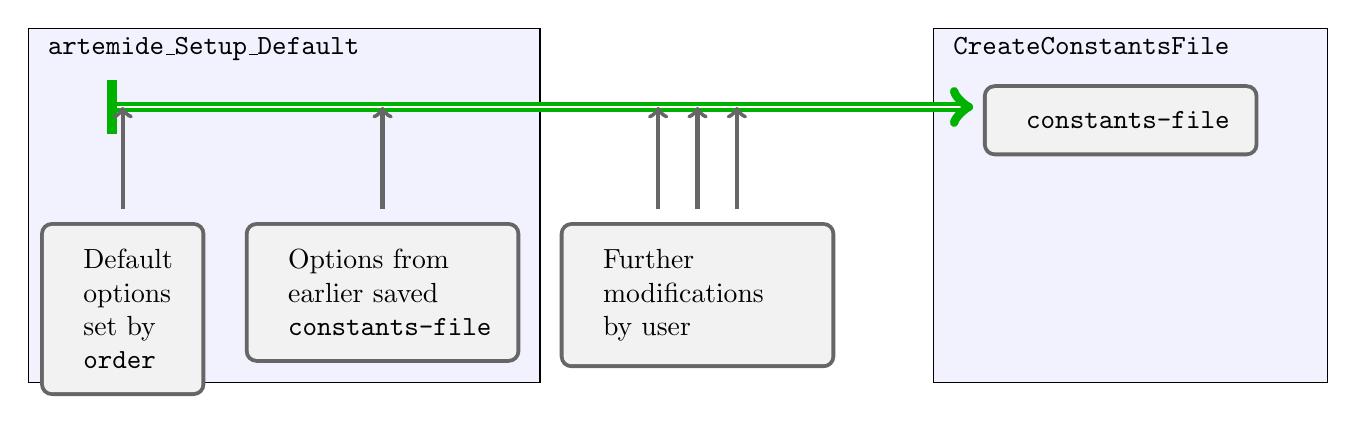
\begin{tikzpicture}

\draw[black,fill=blue!05!white] (-1,3) rectangle (5.5,-1.5);

\node [text width=3.5cm,below] at (1,3){\texttt{artemide\_Setup\_Default}};

\draw[black,fill=blue!05!white] (10.5,3) rectangle (15.5,-1.5);

\node [text width=3.5cm,below] at (12.5,3){\texttt{CreateConstantsFile}};

\draw[|->,green!70!black,ultra thick,double] (0,2) -- (11,2);

\node [text width=3.5cm,right] at (11,2) {
\begin{tcolorbox}[enhanced,colframe=black!60!white,fonttitle=\bfseries,
rightupper=0mm]
\texttt{constants-file}
\end{tcolorbox}};

\draw[->,black!60!white,ultra thick] (0.2,0.7) -- (0.2,2);
\node [text width=2.1cm,below] at (0.2,1) {
\begin{tcolorbox}[enhanced,colframe=black!60!white,fonttitle=\bfseries,
rightupper=0mm]
Default options set by \texttt{order}
\end{tcolorbox}};

\draw[->,black!60!white,ultra thick] (3.5,0.7) -- (3.5,2);
\node [text width=3.5cm,below] at (3.5,1) {
\begin{tcolorbox}[enhanced,colframe=black!60!white,fonttitle=\bfseries,
rightupper=0mm]
Options from earlier saved \texttt{constants-file}
\end{tcolorbox}};


\draw[->,black!60!white,ultra thick] (7,0.7) -- (7,2);
\draw[->,black!60!white,ultra thick] (7.5,0.7) -- (7.5,2);
\draw[->,black!60!white,ultra thick] (8,0.7) -- (8,2);
\node [text width=3.5cm,below] at (7.5,1) {
\begin{tcolorbox}[colframe=black!60!white,fonttitle=\bfseries,
rightupper=0mm]
Further \\ modifications\\ by user
\end{tcolorbox}};


%\draw[->,blue!70!black,ultra thick] (13,1.5) -- (13,-1.25);
%\draw[->,blue!70!black,ultra thick] (13.2,1.5) -- (13.8,-1.25);
%\draw[->,blue!70!black,ultra thick] (12.8,1.5) -- (12.2,-1.25);

%\node [text width=4.5cm,below] at (13,-1) {
%\begin{tcolorbox}[enhanced,colframe=blue!60!white,fonttitle=\bfseries,colback=blue!40!white,
%rightupper=0mm]
%\center Initialization of \\ \texttt{artemide} modules
%\end{tcolorbox}};

\end{tikzpicture}
\caption{\label{fig:create_const} Scheme of creation and modification of \texttt{constants-file} by \texttt{aTMDe\_setup}.}
\end{figure}


\newpage

\section{\texttt{aTMDe\_control} module}
\label{aTMDe_control}

The module \texttt{aTMDe\_setup} is used to coordinate the operation of other modules. It does not bring any new features, just operates other modules in proper order. It is only for convenience.

\begin{center}
List of commands \blue{optional parameters are shown in blue.}
\\
\begin{longtable}{||p{7cm}|c|p{10cm}||}
\hline\hline
Command & Sec. & Short description
\\\hline
\texttt{artemide\_Initialize(file,\blue{prefix,order}) } & \ref{sec:aTMDe_Setup} &  The command which initialize modules according to \texttt{constants-file} created by  \texttt{artemide\_Setup\_fromFile(file,\blue{prefix,order}) }.
\\\hline
\texttt{artemide\_ShowStatistics()} & & Shows some information.
\\\hline
\texttt{artemide\_SetNPparameters(lambdaNP)} &\ref{control:NPparam} & Receive a (real*8)list of NP parameters, split it according to current setup and passes NP parameters to appropriate modules. Reset modules counters.
\\\hline
\texttt{artemide\_SetNPparameters\_TMDR(lambdaNP)} &\ref{control:NPparam} & Reset NP parameters of \texttt{TMDR}-module by (real*8) list \texttt{lambdaNP}. Reset modules counters.
\\\hline
\texttt{artemide\_SetNPparameters\_uTMDPDF(lambdaNP)} &\ref{control:NPparam} & Reset NP parameters of \texttt{uTMDPDF}-module by (real*8) list \texttt{lambdaNP}. Reset modules counters.
\\\hline
\texttt{artemide\_SetNPparameters\_uTMDFF(lambdaNP)} &\ref{control:NPparam} & Reset NP parameters of \texttt{uTMDFF}-module by (real*8) list \texttt{lambdaNP}. Reset modules counters.
\\\hline
\texttt{artemide\_SetNPparameters\_lpTMDFF(lambdaNP)} &\ref{control:NPparam} & Reset NP parameters of \texttt{lpTMDFF}-module by (real*8) list \texttt{lambdaNP}. Reset modules counters.
\\\hline
\texttt{artemide\_SetReplica\_TMDR(num)} &\ref{control:NPparam} & Reset NP parameters of \texttt{TMDR}-module by values corresponding to replica (int)\texttt{num}. Reset modules counters.
\\\hline
\texttt{artemide\_SetReplica\_uTMDPDF(num)} &\ref{control:NPparam} & Reset NP parameters of \texttt{uTMDPDF}-module by values corresponding to replica (int)\texttt{num}. Reset modules counters.
\\\hline
\texttt{artemide\_SetReplica\_uTMDFF(num)} &\ref{control:NPparam} & Reset NP parameters of \texttt{uTMDFF}-module by values corresponding to replica (int)\texttt{num}. Reset modules counters.
\\\hline
\texttt{artemide\_SetReplica\_lpTMDPDF(num)} &\ref{control:NPparam} & Reset NP parameters of \texttt{lpTMDPDF}-module by values corresponding to replica (int)\texttt{num}. Reset modules counters.
\\\hline
\texttt{artemide\_SetScaleVariations(c1,c2,c3,c4)} & - & Change the value of scale-variation constants $c_1-c_4$.
\\\hline\hline
\texttt{artemide\_GetReplicaFromFile(file,rep,array)} & - & Read the .rep file (path is \texttt{file}), and search for the replica (int)\texttt{rep}. Return the (real*8,allocatable)\texttt{array} of NP parameters. \textbf{This command can work without initialization of artemide-control}, in this case, no check of consistency is performed and warning raised.
\\\hline
\texttt{artemide\_NumOfReplicasInFile(file)} & - & Read the .rep file (path is \texttt{file}), and return the number of replicas saved in it.
\end{longtable}
\end{center}

\subsection{Passing non-perturbative parameters}
\label{control:NPparam}

The important part of the initialization is the number of NP parameters for each TMD distributions under consideration. Each TMD-evaluating module (say, \texttt{uTMDPDF}, \texttt{uTMDFF}, etc.) requires $n_i$ number of parameters. The numbers are specified in \texttt{constants-file}. The number must be greater then zero $n_i>0$ for any used module, i.e. $f_{NP}$ is at least 1-parametric (if it is not so, just do not use the parameter in the definition of $f_{NP}$, but keep $n_i>0$). These numbers are read during the initialization procedure, and allocate the memory. 

The set of particular values of these parameters can be done by several ways.

~

\textbf{Option I: } Set all values in a single call

\texttt{call artemide{\_}SetNPParameters(lambda)}

where 
\begin{itemize}
\item[$\{\lambda_i\}$] real*8(1:$\sum_i n_i$ ) The set of parameters which define the non-perturbative functions $f_{NP}$ within modules. It is split into parts and send to corresponding modules. I.e. lambda(1:$n_0$) $\to$\texttt{uTMDR}, lambda($n_0+1$:$n_0+n_1$) $\to$\texttt{uTMDPDF},  lambda($n_0+n_1+1$:$n_0+n_1+n_2$) $\to$\texttt{uTMDFF} (fixed order). 
\end{itemize}

~

\textbf{Option II: } Set value for particular function. For it call \texttt{artemide\_SetNPparameters\_???(lambdaNP)}, where \texttt{???} is module name, e.g.

\texttt{\texttt{artemide\_SetNPparameters\_uTMDPDF(lambdaNP)}}

will set parameters for unpolarized TMDPDF.

~

\textbf{Option III: } You can use presaved values of $\lambda_{NP}$ for a given function. They are provided by model file (if provided). To set NP-input given by integer \texttt{num}, call \texttt{artemide\_SetReplica\_???(num)}, where \texttt{???} is module name, e.g.

\texttt{\texttt{artemide\_SetReplica\_uTMDPDF(num)}}

will set parameters for unpolarized TMDPDF.

\newpage

\section{\texttt{QCDinput} module}
\label{QCDinput}

The module \texttt{QCDinput} gives an interface to external function provided by the user, such as PDF, FF, values of alpha-strong. It is completely user defined. In particular, in the default version it is linked to LHAPDF library \cite{Buckley:2014ana}.

\begin{center}
List of available commands \blue{optional parameters are shown in blue.}
\\
\begin{tabular}{||l|p{10cm}||}
\hline\hline
Command~~~~~~~~~~~~~~~~~~~~~~~~~~~~~~~ & Description
\\\hline
\texttt{QCDinput{\_}Initialize(file,\blue{prefix})} & Subroutine to initialize anything what is needed. (string) \texttt{file} is the name of \texttt{constants-file}, which contains initialization information. (string)\texttt{prefix} is appended to \texttt{file} if provided.
\\\hline
\texttt{As(Q)} &  Returns the (real*8) value of $\alpha_s(Q)/(4\pi)$. $Q$ is (real*8).
\\\hline
\texttt{xPDF(x,Q,hadron)} &  Returns the (real*8(-5:5)) value of $xf(x,Q)$ for given hadron. \texttt{x, Q} are (real*8), \texttt{hadron} is (integer).
\\\hline
\texttt{xFF(x,Q,hadron)} &  Returns the (real*8(-5:5)) value of $xd(x,Q)$ for given hadron. \texttt{x, Q} are (real*8), \texttt{hadron} is (integer).
\\\hline
\texttt{x\_hPDF(x,Q,hadron)} &  Returns the (real*8(-5:5)) value of $xg_1(x,Q)$ for given hadron ($g_1$=helicity distribution). \texttt{x, Q} are (real*8), \texttt{hadron} is (integer).
\\\hline
\texttt{mCHARM} &  (real*8)Constant for mass of charm quark.
\\\hline
\texttt{mBOTTOM} &  (real*8)Constant for mass of bottom quark.
\\\hline\hline
\texttt{QCDinput\_SetPDFreplica(num,h)} & Changes the unpolarized PDF replica number for hadron \texttt{h} to \texttt{rep}.
\\\hline
\texttt{QCDinput\_SetFFreplica(num,h)} & Changes the unpolarized FF replica number for hadron \texttt{h} to \texttt{rep}.
\\\hline
\texttt{QCDinput\_SetlpPDFreplica(num,h)} & Changes the replica of PDF associated with linearly polarized gluon PDF number for hadron \texttt{h} to \texttt{rep}.
\\\hline
\texttt{QCDinput\_SethPDFreplica(num,h)} & Changes the replica of helicity PDF number for hadron \texttt{h} to \texttt{rep}.
\\\hline\hline
\end{tabular}
\end{center}

\subsection{Initialization}
\label{sec:QCDinput_ini}

\red{TOBE WRITTEN}

\newpage
\section{\texttt{EWinput} module}
\label{EWinput}

\texttt{EWinput} module contains definitions of various physical parameters of elector-weak interactions, such as masses of Z and W bosons, CKM matrix, code for evolution of $\alpha_{QED}$ etc.

\red{TOBE WRITTEN}

\subsection{$\alpha_{\text{QED}}$}

\textbf{This implementation has been added in ver.2.03. In earlier versions the code for $\alpha_{\text{QED}}$ had a bug that generated slightly lower values (independently on the values of $\mu$).}

The QED coupling constant is set by the one-loop QED evolution with LO matching at thresholds. In order to tune it finer, the value of $\beta_0$ is modified by $\beta_0\to \beta_0+\delta \beta$, where $\delta \beta$ is found by exact implementation of two boundary values, $\alpha_{\text{QED}}(m_\tau)$ and $\alpha_{\text{QED}}(m_Z)$. 

The LO evolution is
\begin{eqnarray}
\alpha(\mu)=\frac{1}{\alpha_0^{-1}+2\beta_0 \ln(\mu/\mu_0)},
\end{eqnarray}
where $\beta_0=-(3\pi)^{-1}N_{eff}$ with 
\begin{eqnarray}
N_{eff}=\sum_{\substack{\text{active}\\\text{ leptons}}}1+N_c\sum_{\substack{\text{active}\\\text{quarks}}}e_q^2.
\end{eqnarray}
In artemide I account the following threasholds
\begin{center}
\begin{tabular}{c||c|c|c|c|c|c|c|}
$\mu$   & $\mu<m_e(\sim m_u,m_d)$ & $\mu<m_\mu(\sim m_s)$ & ~$\mu<m_c$~ & ~$\mu<m_\tau$~ & ~$\mu<m_b$~ & ~$\mu<m_t$~ & $\mu>m_t$
\\\hline
$N_{eff}$& 0 & $\frac{8}{3}$ & $4$ & $\frac{16}{3}$ & $\frac{19}{3}$ & $\frac{20}{3}$ & $8$ 
\end{tabular}
\end{center}
So the actual formula for $\alpha_{QED}$ is
\begin{eqnarray}
\alpha_{\text{QED}}(\mu)=\frac{1}{\alpha_Z^{-1}+2\bar \beta\[N_{eff}(\mu)\ln\(\frac{\mu}{m_{th}}\)+\sum_{m_i\in m_{th}} N_{eff}\ln\(\frac{m_{i}}{m_{i+1}}\)\]},
\end{eqnarray}
where $m_{th}$ are all threasholds from $\mu$ till $M_Z$. The constant $\bar \beta$ is defined by exact matching at $M_Z$ and $m_\tau$. For default values $\bar\beta/\beta_0\sim 1.002\%$, so it accounts for really tiny effects.

\newpage

\section{TMD evolution modules}

The TMD evolution has several implementation. The artemide v3 (and higher) is hard-coded to use the fixed-$\mu$ evolution (see ref.\cite{Scimemi:2018xaf}). This choice is made after many test performed in earlier versions or artemide (where the type of evolution was selected by user), and the demonstration that they are equivalent within perturbative uncertainty.

The fixed-$\mu$ scale corresponds to evolution along $\zeta$ is with fixed-$\mu$ solution to the special equi-potential line, and evolution along $\mu$ along equi-potential line (this part is unity by definition). The evolution factor reads
\begin{eqnarray}
R[b,(\mu_1,\zeta_1)\to(\mu_2,\zeta_2)]&=&\frac{R[b,(\mu_1,\zeta_1)\to(\mu_1,\zeta_{\mu_1})]}{R[b,(\mu_2,\zeta_2)\to(\mu_2,\zeta_{\mu_2})]},
\\
R[b,(\mu,\zeta)\to(\mu,\zeta_{\mu})]&=&\exp\(-\mathcal{D}(\mu,b)\ln\(\frac{\zeta}{\zeta_\mu(b)}\)\),
\end{eqnarray}
where $\mathcal{D}$ is the Collins-Soper kernel, and $\zeta_\mu(b)$ is the special $\zeta$-line.

The Collins-Soper kernel is defined as
\begin{eqnarray}
\mathcal{D}^f(\mu,b)=\mathcal{D}^f_{\text{pert}}(\mu_{\text{OPE}},b)+\int_{\mu_{\text{OPE}}}^{\mu} \frac{d\mu'}{\mu'}\Gamma^f(\mu')+\mathcal{D}^f_{\text{NP}}(b),
\end{eqnarray}
where $\mathcal{D}^f_{\text{pert}}$ is the high-scale perturbative part, and $\mathcal{D}_{\text{NP}}$ is the non-perturbative model (e.g. $g_Kb^2$)

The module for evolution includes three modules
\begin{itemize}
\item \texttt{TMD\_AD} this module contains collection of all anomalous dimensions and related quantities. Logically it is equivalent to \texttt{\_OPE} modules.
\item \texttt{TMDR\_model} this module contains the user-defined non-perturbative input.
\item \texttt{TMDR} this module interface \texttt{TMD\_AD} and \texttt{TMDR\_model} into the evolution factor, and perform the general control.
\end{itemize}
The initialization is happened thorough the \texttt{TMDR}-module.

At small values of parameter $Q=Q_0$ the point $(Q,Q^2)$ crosses the $\zeta$-lines. The value of $Q_0$ depends on $b$. The dangerous situation is then hard scale of the process $Q$ is smaller then $Q_0$ at large $b=b_\infty$. In this case the evolution kernel $R[b_\infty,(Q,Q^2)\to \zeta_\mu]>1$, which is generally implies that it grows to infinity. However, it happens only at small values of $Q$. E.g. at NNLO the typical value of $Q_0$ is $\sim 1.5$GeV. That should be taken into account during consideration of low-energy experiment and especially their error-band, since the point $(c_2Q,Q^2)$ could cross the point at larger values of $Q$.

The function \texttt{LowestQ()} returns the values (real*8(1:3)) $\{Q_{-1},Q_0,Q_{+1}\}$, which are solution of equation $Q^2=\zeta_{c Q}(b)$, for (fixed bu) large values of $b$. $Q_{-1}$ corresponds to $c=0.5$, $Q_0$ corresponds to $c=1$ and $Q_{+1}$ corresponds to $c=2$.

\subsubsection{INI-parameters}

\begin{center}
\textbf{Parameters for TMD-evolution modules (section \texttt{*3}).} 
\\
\begin{tabular}{||p{1.5cm}||c||p{12.5cm}||}
\hline\hline
Entry &~~Type~~& Description
\\\hline
A.p1 & str & Order of the evolution \textit{standardized}. Could be LO, NLO,.. (see table below for details)
\\\hline
A.p2 & T/F & The flag to override the \textit{standard} evolution definition. If T, than instead of A.p1 the orders defined in A.p3 -- A.p6 are used.
\\\hline
A.p3 & str & Order of $\Gamma_{\text{cusp}}$. LO=$a_s \Gamma_0$, NLO=$a_s \Gamma_0+a_s^2\Gamma_1$, etc.
\\\hline
A.p4 & str & Order of $\gamma_{V}$. LO=0, NLO=$a_s \gamma_1$, etc.
\\\hline
A.p5 & str & Order of $\mathcal{D}_{\text{pert}}$. LO=0, NLO=$a_s \mathbf{L}+d^{(1,0)}$, etc.
\\\hline
A.p6 & str & Order of $\zeta_\mu$ (exact solution). LO=$a_s^0$*(exact solution),  etc.
\\\hline\hline
B.p1 & int & Number of NP parameters.
\\\hline\hline
C.p1 & real & Tolerance general (used for check of variable modifications, etc. Does not affect integration precision). (default =$10^{-6}$)
\\\hline
C.p2 & real & Small-b value at which the evolution is frozen (default =$10^{-6}$)
\\\hline
C.p3 & real & Parameter for smoothing the small-b value of exact $\zeta$-line (see below) (default =$0.01$).
\\\hline\hline
\end{tabular}
\end{center}

\begin{center}
The table of correspondence between \texttt{standard} definition and particular definitions
\begin{tabular}{|l||c|c|c||c|| c|}
\texttt{order}~~~ & ~~$\Gamma_{\text{cusp}}$~~ & ~~$\gamma_V$~~ & ~~$\mathcal{D}$~*~ & ~~$\mathcal{D}_{\text{resum}}$~~ & ~~$\zeta_\mu$~**~
\\\hline\hline
\texttt{LO} & $a_s^1$ & $a_s^0$ & $a_s^0$ & $a_s^0$ & $a_s^0$ 
\\\hline
\texttt{NLO} & $a_s^2$ & $a_s^1$ & $a_s^1$ & $a_s^1$ & $a_s^2$ 
\\\hline
\texttt{NNLO}=\texttt{N2LO} & $a_s^3$ & $a_s^2$ & $a_s^2$ & $a_s^2$ & $a_s^3$ 
\\\hline
\texttt{NNNLO}=\texttt{N3LO} & $a_s^4$ & $a_s^3$ & $a_s^3$ & $a_s^2$ & $a_s^4$ 
\\\hline
\texttt{N4LO} & $a_s^5$ & $a_s^4$ & $a_s^4$ & $a_s^3$ & ${a_s^5}^{***}$ 
\\\hline
\end{tabular}
\end{center}

\begin{itemize}
\item[*] $\mathcal{D}_{\text{resum}}$ starts from $a_s^0$, it already contains $\Gamma_0$.
\item[**] Definition of $\zeta_\mu$ is correct only in the natural ordering, i.e. \texttt{LO},\texttt{NLO},\texttt{NNLO}. Proper definition in \texttt{+} orders would make the function too heavy. The resumed version has the same counting.
\item[***] The finite part =0, since $d^{(5,0)}$ is unknown.
\end{itemize}

\textbf{Notes:}
\begin{itemize}
\item For very small-values of $b$ the value of $b$ is fixed.
\item For very large positive values of $\mathcal{D}$ (i.e. for $b>25$GeV$^{-1}$ or so), the exact solution for $\zeta$-line diverges exponentially at 3- and 4- loops. It is because the coefficient infront of rising terms is negative. To prevent the divergence, the corresponding terms are expanded in $a_s$ up to needed power ($\alpha_s^6$).
\end{itemize}

\subsubsection{Functions}

\begin{center}
\texttt{XX}=name of module (e.g. \texttt{uTMDPDF}, \texttt{uTMDFF}, etc.)
\\
\begin{tabular}{||p{5.5cm}||c||p{8.5cm}||}
\hline\hline
Entry &~~Type~~& Description
\\\hline
\texttt{TMDR\_Initialize(file,prefix)} & subroutine & Initialize the module from INI-file.
\\\hline
\texttt{TMDR\_SetScaleVariation(c1)} & subroutine & Sets globally a new value for constant $c_1$.
\\\hline
\texttt{TMDR\_SetNPparameters(lambda)} & subroutine & Set a new vector of NP parameters $\lambda_{\text{NP}}$. The new vector must be same size as declared at the setup.
\\\hline
\texttt{TMDR\_CurrentNPparameters()} & real(:) & Returns the current vector for $\lambda_{\text{NP}}$.
\\\hline\hline
\texttt{CS\_kernel(mu,b,f)} & real & Returns the value Collins-Soper kernel at scale $\mu$, point $b$ for flavor $f$.
\\\hline
\texttt{zetaNP(mu,b,f)} & real & Returns the value $\zeta_\mu$ for give CS kernel at scale $\mu$, point $b$ for flavor $f$.
\\\hline
\texttt{TMDR\_Rzeta(b,muf,zetaf,f)} & real & Return the factor $R$ for evolution from the point $(\mu,\zeta)$ down to the special evolution line.
\\\hline
\texttt{TMDR\_R(b,muf,zetaf,mui,zetai,f)} & real & Return the factor $R$ for evolution from the point $(\mu_f,\zeta_f)$ to $(\mu_i,\zeta_i)$.
\\\hline
\texttt{LowestQ()} & real & Attempts to compute the lowest available scale $Q$, for which the evolution converges.
\\\hline\hline
\end{tabular}
\end{center}

\subsection{\texttt{TMD\_AD} module}
\label{TMD_AD}

The module \texttt{TMD\_AD} give access to various perturbative anomalous dimensions needed for TMD evolution. This module is essential part of \texttt{TMDR} module, and thus initialized by it. 

\begin{center}
List of available commands
\\
\begin{tabular}{||l|c|p{10cm}||}
\hline\hline
Command & ~~Sec.~~ & Short description
\\\hline
\texttt{TMD\_AD\_Initialize(oC,oV,oD,oDr,oZ) } & \ref{TMDR:init} & Initialization of module. The (integer) parameters (\texttt{oC,oV,oD,oDr,oZ}) are orders of definition for anomalous dimensions ($\Gamma_{\text{cusp}}$, $\gamma_V$, $\mathcal{D}_{\text{pert}}$, $\mathcal{D}_{\text{resum}}$, $\zeta_{\text{pert}}$).
\\\hline
\texttt{GammaCusp(mu,f)} &  & $=\Gamma_{\text{cusp}}^f(\mu)$
\\\hline
\texttt{gammaV(mu,f)} &  & $=\gamma_V^f(\mu)$
\\\hline
\texttt{Dpert(mu,bT,f)} &  & $=\mathcal{D}_{\text{pert}}^f(b,\mu)$
\\\hline
\texttt{Dresum(mu,bT,f)} & &  $=\mathcal{D}_{\text{resum}}^f(b,\mu)$
\\\hline
\texttt{zetaMUpert(mu,bT,f)} &  & $=\zeta_{\text{pert}}^f(b,\mu)$
\\\hline
\texttt{zetaSL(mu,rad,f)} & &  $=\zeta_{\text{exact}}^f(\mathcal{D},\mu)$ (\blue{Note, the argument.})
\\\hline
\texttt{RADEvolution(mu0,mu1,f)} & &  $=\int_{\mu_0}^{\mu_1} \frac{d\mu^2}{\mu^2}\frac{\Gamma(\mu)}{2}$ The evolution constant for $\mathcal{D}$
\\
\hline\hline
\end{tabular}
\end{center}

\textbf{Notes:}
\begin{itemize}
\item The integral over $\mu$ is done using exact analytical formula by decomposition of $\beta$-function over roots. 
\item The exact expression for $\zeta$-line is numerically unstable at very small-$b$. It is due to its double-exponential nature which requires exponentiation and cancellation of large-numbers. However, it could be computed analytically in this regime as expansion. Thus, to stabilize the computation of expression the following formula is used
\begin{eqnarray}
\zeta_\mu = e^{-b^2/S}\zeta_\text{pert}+(1-e^{-b^2/S})\zeta_\text{exact}.
\end{eqnarray}
Here, $S$ is the smoothing parameter. It should be small enough to guaranty non-impact of approximation (approx. $S<0.05$).
\end{itemize}

\subsection{\texttt{TMDR\_model}}

\begin{tcolorbox}
\begin{center}
\textbf{This module gives the expression for $\mathcal{D}$. It could be modified by user, and one of modules that form a TMD model (together with models for TMD-distributions).}
\\
\textbf{\blue{Making this module follow the interface}}
\end{center}
\texttt{public:: ModelInitialization(NPlength)}
\\
\texttt{public:: ModelUpdate(NParray)}
\\
\texttt{real(dp),public:: DNP(b,f)}
\\
\texttt{real(dp),public:: bSTAR(b)}
\\
\texttt{real(dp),public:: muOPE(b,c1)}
\end{tcolorbox}

\texttt{ModelInitialization(NPlength)}: this subroutine is called during the initialization of \texttt{TMDR}. The \texttt{integer,intent(in)::NParray(:)} is the length of array of NP-parameters. Use this subroutine to make preparation of the model.

\vspace{2mm}

\texttt{ModelUpdate(NParray)}: this subroutine is called during the \texttt{TMDR\_setNPparameters(NParray)}. The \texttt{real(dp),intent(in)::NParray(:)} is the array of NP-parameters passed to \texttt{TMDR\_setNPparameters}. Use this subroutine to recompute model parameters (if needed), save NP-parameters (if needed), etc.

\vspace{2mm}

\texttt{DNP(b,f)}: the function returns the value, $\mathcal{D}^f_{\text{NP}}(b)$. It contains only NP part. 

\vspace{2mm}

\texttt{bSTAR(b)}: the function returns the value, $b^*(b)$ used instead of $b$ within $\mathcal{D}_{\text{pert}}$

\vspace{2mm}

\texttt{muOPE(b,c1)}: the function returns the value, $\mu_{\text{OPE}}$ used as reference scale of $\mathcal{D}_{\text{pert}}$. The parameter $c_1$ is the prescription used during the scale variation.

\vspace{2mm}

\textbf{Important:} the module \texttt{TMDR\_model} is compiled before \texttt{TMDR}, and thus can use only lower-level modules: \texttt{TMD\_AD, QCDinput,} etc.


\newpage

\section{Modules computing TMD distributions}

There are many TMD distributions each computed in a separate module. All TMD distributions are split in the following classes:
\begin{itemize}
\item \textbf{Pure Twist-2 OPE} These are \texttt{uTMDPDF}, \texttt{uTMDFF}, \texttt{lpTMDPDF}. These TMD distributions are defined by twist-2 collinear distribution at small-b
\item \textbf{Pure Twist-3 OPE} These are \texttt{SiversTMDPDF}, \texttt{BoerMuldersTMDPDF}. These TMD distributions are defined by twist-3 collinear distribution at small-b
\item \textbf{Twist-2 \& Twist-3 OPE} These are \texttt{wgtTMDPDF}. These TMD distributions are defined by twist-2 (WW-term) and twist-3 collinear distribution at small-b
\end{itemize}
These lists are to be extended in the future. 

Each module consists of several sub-modules, which have names as \texttt{TMDname\_X}. The \texttt{X} corresponds to
\begin{itemize}
\item  \texttt{OPE} this module computes the convolution of the twist-2 (or twist-3) coefficient function with corresponding PDF.
\item \texttt{model} this module contains all information about NP-part and other free-parameters (such as $\mu_{\text{OPE}}$ of the given TMD distribution. \textbf{\blue{These modules could be edited by user, to implement/update/fit TMDs.}}
\end{itemize}

The most part of modules are identical. There are a few differences in the implementation. So, first the general structure is presented, and then particularities.

Different OPE's are known up to different orders. Consequently, the modules implement them at different orders. The orders are denoted as
\begin{eqnarray*}
\texttt{NA}&:\to & \text{no OPE}
\\
\texttt{LO}&:\to & C=\mathcal{O}(a_s^0)
\\
\texttt{NLO}&:\to & C=\mathcal{O}(a_s^1)
\\
\texttt{NNLO}=\texttt{N2LO}&:\to & C=\mathcal{O}(a_s^2)
\\
\texttt{NNNLO}=\texttt{N3LO}&:\to & C=\mathcal{O}(a_s^3).
\end{eqnarray*}
\begin{itemize}
\item The \texttt{NA} option is used to remove any relation to collinear distributions. In this case $TMD(x,b)=f_{\text{NP}}(x,b)$
\item If the coefficient function at LO/NLO/.. is zero, the convolution is also zero. E.g. linearly polarized gluons start at $\sim a_s$, the convolution is zero at \texttt{LO}. 
\end{itemize}
\begin{center}
List of available orders for different distributions
\end{center}
\begin{eqnarray*}
\texttt{uTMDPDF}&:& \texttt{NA, LO, NLO, N2LO, N3LO}
\\
\texttt{uTMDFF}&:& \texttt{NA, LO, NLO, N2LO, N3LO}
\\
\texttt{lpTMDPDF}&:& \texttt{NA, LO, NLO, N2LO}
\\
\texttt{wgtTMDPDF}[tw2]&:& \texttt{NA, LO, NLO}
\\
\texttt{wgtTMDPDF}[tw3]&:& \texttt{NA}
\\
\texttt{SiversTMDPDF}[tw3]&:& \texttt{NA}
\\
\texttt{BoerMuldersTMDPDF}[tw3]&:& \texttt{NA}
\end{eqnarray*}

The functions are computed by the following rule
\begin{eqnarray}
\texttt{uTMDPDF}&=&[C\times f]_{\text{tw2}}(x,b)F_{\text{NP}}(x,b),
\\
\texttt{uTMDFF}&=&[C\times d]_{\text{tw2}}(x,b)F_{\text{NP}}(x,b),
\\
\texttt{lpTMDPDF}&=&[C\times f]_{\text{tw2}}(x,b)F_{\text{NP}}(x,b),
\\
\texttt{wgtTMDPDF}&=&[C\times h]_{\text{tw2}}(x,b)F_{\text{NP}}(x,b)+[C\times T]_{\text{tw3}}(x,b)F^{\text{tw3}}_{\text{NP}}(x,b),
\\
\texttt{SiversTMDPDF}&=&[C\times T]_{\text{tw3}}(x,b)F^{\text{tw3}}_{\text{NP}}(x,b),
\\
\texttt{BoerMuldersTMDPDF}&=&[C\times E]_{\text{tw3}}(x,b)F^{\text{tw3}}_{\text{NP}}(x,b),
\end{eqnarray}
where $f$, $d$, $h$ are collinear distributions of twist-2, and $[C\times h]_{\text{tw2}}$ is corresponding convolution;
$T$ and $E$ are collinear distributions of twist-3, and $[C\times T]_{\text{tw3}}$, $[C\times E]_{\text{tw3}}$ are corresponding convolution; $F_{\text{NP}}(x,b)$ and $F^{\text{tw3}}_{\text{NP}}(x,b)$ are non-perturbative functions to be fit. NP functions are defined in the \texttt{XX\_model} modules, and share the same $\lambda_{\text{NP}}$ (array of parameters). This structure correctly reproduces the small-b properties of TMD-distributions. The convolutions are computed in separate modules see sec.\ref{TMD_OPE}, \ref{TMD_OPE_tw3}.

The modules computes the optimal TMDs, and also evolved TMDs. Generally a TMD distribution is given by the expression
\begin{eqnarray}\label{TMD:F=RF}
F_f(x,b;\mu,\zeta)=R_f[b,(\mu,\zeta)\to(\mu,\zeta_{\mu})]\tilde F_f(x,b),
\end{eqnarray}
where $R$ is the TMD evolution kernel, $\tilde F$ is an optimal TMD distribution. 

\subsubsection{INI-parameters}

\begin{center}
\textbf{Parameters universal for all such modules which include only tw2 or tw3 OPE (mixed case see below).} 
\\
\begin{tabular}{||p{1.5cm}||c||p{12.5cm}||}
\hline\hline
Entry &~~Type~~& Description
\\\hline
\\\hline\hline
A.p1 & T/F & Include gluon into the computation. Usually gluon is computed by a separate rule, and switching off this option leads to $\sim 2$ increase in the computation velocity.
\\\hline
A.p2 & in & Number of hadrons. Specify maximum required number of hadrons.
\\\hline\hline
B.p1 & str & Order of the coefficient function. Could be N/A, LO, NLO,.. (see table below for details)
\\\hline
B.p2 & T/F & Trigger to prepare the grid (T=prepare). Preparation is done on the initialization stage.
\\\hline
B.p3 & T/F & Trigger the test of the grid (T=run the test). Take the same time as computation of the grid (by a single processor). Requires A.p2=T. Example Result is shown in sec.\ref{sec:OPE:grid1}. 
\\\hline\hline
C.p1 & int & Number of NP parameters.
\\\hline
C.p2 & real & $B_{\text{MAX-ABS}}$, a large number such that $b>B_{\text{MAX-ABS}}$ the TMD is returned 0. (default 100).
\\\hline\hline
D.p1 & real & Tolerance for integration (default =$10^{-6}$)
\\\hline
D.p2 & real & Tolerance general (used for check of variable modifications, etc. Does not affect integration precision). (default =$10^{-6}$)
\\\hline
D.p3 & int & Maximum number of iteration for adaptive integration. (default =$10^{4}$)
\\\hline\hline
E.p1 & real & $x_{\text{min}}$ for the grid (see (\ref{OPE:x-grid}))
\\\hline
E.p2 & real & $p_x$ for the grid (see (\ref{OPE:x-grid}))
\\\hline
E.p3 & real & $b_{\text{min}}$ for the grid (see (\ref{OPE:b-grid})). [It is not related to parameter $b_{\min}$ of $b^*$-prescription!]
\\\hline
E.p4 & real & $b_{\max}$ for the grid (see (\ref{OPE:b-grid})) [It is not related to parameter $b_{\max}$ of $b^*$-prescription!]
\\\hline
E.p5 & integer & Number of nodes in the x-grid
\\\hline
E.p6 & integer & Number of nodes in the b-grid
\\\hline\hline
F.p1 & real & Tolerance use in the Fourier integral to the $k_T$-space (default =$10^{4}$)
\\\hline
F.p2 & real & Step for the Ogata quadrature (default =$10^{-3}$)
\\\hline
F.p3 & real & Minimal $k_T$ to compute. Below this number distribution is frozen. (default =$10^{-4}$)
\\\hline\hline
G.p1 & real & Tolerance use in the Fourier integral for TMM (default =$10^{4}$)
\\\hline
G.p2 & real & Step for the Ogata quadrature for TMM computation (default =$10^{-3}$)
\\\hline
G.p3 & real & Minimal $\mu$ to compute. Below this number the program terminates. (default =$0.8$GeV)
\\\hline\hline
\end{tabular}
\end{center}
\begin{itemize}
\item \texttt{wgtTMDPDF} has extra section F and G, which are analogous to sections B and C, but responsible for twist-3 convolution. The section F,G,I is correspondingly sections H,I.
\end{itemize}

\subsubsection{Functions}

\begin{center}
\texttt{XX}=name of module (e.g. \texttt{uTMDPDF}, \texttt{uTMDFF}, etc.)
\\
\begin{tabular}{||p{5.5cm}||c||p{8.5cm}||}
\hline\hline
Entry &~~Type~~& Description
\\\hline
\texttt{XX\_Initialize(file,prefix)} & subroutine & Initialize the module from INI-file.
\\\hline
\texttt{XX\_SetPDFreplica(rep,h)} & subroutine & Passes to \texttt{XX\_OPE\_SetPDFreplica}
\\\hline
\texttt{XX\_SetScaleVariation(c4)} & subroutine & Passes to \texttt{XX\_OPE\_SetScaleVariation}
\\\hline
\texttt{XX\_SetLambdaNP(lambda)} & subroutine & Set a new vector of NP parameters $\lambda_{\text{NP}}$. The new vector must be same size as declared at the setup.
\\\hline
\texttt{XX\_CurrentLambdaNP()} & real(:) & Returns the current vector for $\lambda_{\text{NP}}$.
\\\hline\hline
\texttt{XX\_lowScale5(x,bT,h)} & real(-5:5) & \red{TO BE REMOVED} Returns the value of TMD distributions for given (x,b) (reals) and hadron h. The value is the vector over flavors. For $h<0$ the quark-distributions are replaced by anti-quark distributions and vice versa. I.e. $F(-h)=F(h)(5:-5:-1)$
\\\hline\hline
\texttt{XX\_inB(x,bT,h)} & real(-5:5) & Returns the value of \blue{optimal} TMD distributions for given (x,b) (reals) and hadron h. The value is the vector over flavors. For $h<0$ the quark-distributions are replaced by anti-quark distributions and vice versa. I.e. $F(-h)=F(h)(5:-5:-1)$
\\\hline
\texttt{XX\_inB(x,bT,mu,zeta,h)} & real(-5:5) & Returns the value of \blue{evolved} TMD distributions (see (\ref{TMD:F=RF})) for given (x,b,$\mu$,$\zeta$) (reals) and hadron h. The value is the vector over flavors. For $h<0$ the quark-distributions are replaced by anti-quark distributions and vice versa. I.e. $F(-h)=F(h)(5:-5:-1)$. $\mu$ is in GeV. $\zeta$ in GeV$^2$.
\\\hline
\texttt{XX\_inKT(x,kT,h)} & real(-5:5) & Returns the value of \blue{optimal} TMD distributions \blue{in momentum space} (see sec.\ref{sec:Fourier_to_kt}) for given (x,$k_T$) (reals) and hadron h. The value is the vector over flavors. For $h<0$ the quark-distributions are replaced by anti-quark distributions and vice versa. I.e. $F(-h)=F(h)(5:-5:-1)$
\\\hline
\texttt{XX\_inKT(x,bT,mu,zeta,h)} & real(-5:5) & Returns the value of \blue{evolved} TMD distributions (see (\ref{TMD:F=RF})) \blue{in momentum space} (see sec.\ref{sec:Fourier_to_kt}) for given (x,$k_T$,$\mu$,$\zeta$) (reals) and hadron h. The value is the vector over flavors. For $h<0$ the quark-distributions are replaced by anti-quark distributions and vice versa. I.e. $F(-h)=F(h)(5:-5:-1)$. $\mu$ is in GeV. $\zeta$ in GeV$^2$.
\\\hline
\texttt{XX\_TMM\_G(x,mu,h)} & real(-5:5) & Returns the value of TMM $\mathcal{G}_{n,n}$ (see sec.\ref{sec:TMM}) for given (x,$\mu$) (reals) and hadron h. The value is the vector over flavors. For $h<0$ the quark-distributions are replaced by anti-quark distributions and vice versa.
\\\hline
\texttt{XX\_TMM\_X(x,mu,h)} & real(-5:5) & Returns the value of TMM $\mathcal{G}_{n+1,n}$ (see sec.\ref{sec:TMM}) for given (x,$\mu$) (reals) and hadron h. The value is the vector over flavors. For $h<0$ the quark-distributions are replaced by anti-quark distributions and vice versa.
\\\hline\hline
\end{tabular}
\end{center}

\begin{center}
\textbf{Functions unique for particular modules}
\\
\begin{tabular}{||p{5.5cm}||c||p{8.5cm}||}
\hline\hline
Entry &~~Type~~& Description
\\\hline
\texttt{uPDF\_uPDF(x1,x2,} \texttt{bt,mu,zeta,h1,h2)} & real(-5:5) & Returns the value of product $f_q f_{\bar q}$ evolved unpolarized TMD distributions for given (x,b) (reals) and hadrons $h_1$ and $h_2$. The value is the vector over flavors. If $h_{1,2}$ have the same sign the product is $f_q f_{\bar q}$, if $h_{1,2}$ have different signs the product is $f_q f_{q}$. This combination is used to compute Drell-Yan-type processes, and a bit faster than a direct multiplication.
\\\hline\hline
\end{tabular}
\end{center}

\newpage
\subsection{\texttt{\_model} modules}
\begin{center}
\blue{\textbf{same for}} \texttt{uTMDFF\_model} and \texttt{lpTMDPDF\_model}.
\end{center}

\begin{tcolorbox}
\begin{center}
\textbf{This module gives the expression for $f_{NP}$, $\mu_{\text{OPE}}$ and $b^*$. It could be written by user, and one of modules that form a TMD model (together with models for TMD-evolution).}
\\
\textbf{\blue{Making this module follow the interface}}
\end{center}
\texttt{public:: ModelInitialization}
\\
\texttt{public:: ModelUpdate}
\\
\texttt{real(dp),public,dimension(-5:5):: FNP}
\\
\texttt{real(dp),public:: bSTAR}
\\
\texttt{real(dp),public:: muOPE}
\\
If there is a twist-3 part of small-b matching, there are extra functions
\\
\texttt{real(dp),public,dimension(-5:5):: FNP\_tw3}
\\
\texttt{real(dp),public:: bSTAR\_tw3}
\\
\texttt{real(dp),public:: muOPE\_tw3}
\\
which contribute to the twist-3 term.
\end{tcolorbox}

\texttt{ModelInitialization(NParray)}: this subroutine is called during the initialization of \texttt{XX} module. The \texttt{integer,intent(in)::NPlength(:)} is the size of the array of NP-parameters. Use this subroutine to make preparation of the model.

\vspace{2mm}

\texttt{ModelUpdate(NParray)}: this subroutine is called during the \texttt{XX\_setNPparameters(NParray)}. The \texttt{real(dp),intent(in)::NParray(:)} is the array of NP-parameters passed to \texttt{TMDR\_setNPparameters}. Use this subroutine to recompute model parameters (if needed), save NP-parameters (if needed), etc.

\vspace{2mm}

\texttt{FNP(x,b,hadron,lambdaNP)}: the function returns $f^{f,h}_{NP}(x,b,\lambda)$. 

\vspace{2mm}

\texttt{bSTAR(b,x,y)}: the function returns $b^*(b)$ function.

\vspace{2mm}

\texttt{mu\_OPE(b,x,y,c4)}: the function returns $\mu_\text{OPE}(z,b)$ function.

\textbf{Important:} the module \texttt{XX\_model} is compiled before \texttt{XX}, and thus can use only lower-level modules: \texttt{TMD\_AD, QCDinput,} etc.

\subsection{\texttt{\_OPE} modules (tw2)}
\label{TMD_OPE}

OPE modules compute the following convolution
\begin{eqnarray}\label{OPE:tw2:main}
[C\times f](x)&=&\int_x^1 \frac{dy}{y} C(y,\mathbf{L})f\(\frac{x}{y},\mu_{\text{OPE}}\)
\\
&=&
\frac{1}{x}\int_x^1 dy C(y,\mathbf{L})F\(\frac{x}{y},\mu_{\text{OPE}}\),
\end{eqnarray}
where $F(x)=xf(x)$ and 
\begin{eqnarray}
\mathbf{L}=\ln\(\frac{\mu^2_{\text{OPE}}b^2}{4e^{-2\gamma_E}}\).
\end{eqnarray}

\begin{tcolorbox}
\begin{center}
OPE modules are initialized automatically from the corresponding TMD module.
\end{center}
\end{tcolorbox}

\textbf{Extra notes:}
\begin{itemize}
\item The convolution is convergent, but the convolution kernel has singularity at $y\to1$. To stabilize the integral, it is computed as
\begin{eqnarray}
\int_x^1 dy (...)=\int_x^{y_C} dy (...)+\int_{y_C}^1 dy (...).
\end{eqnarray}
The first term is computed by the adaptive algorithm. The second term is computed by the approximate formulas
\begin{eqnarray*}
&& \int_{y_C}^1 dy \frac{f(x/y)-f(x)}{1-y}=f(x/y_C)-f(x),
\\
&&\int_{y_C}^1 dy \frac{f(x/y)-f(x)}{1-y}\ln(1-y)=(f(x/y_C)-f(x))(\ln(1-y_C)-1),
\\
&&\int_{y_C}^1 dy \frac{f(x/y)-f(x)}{1-y}\ln^2(1-y)=(f(x/y_C)-f(x))(2-\ln(1-y_C)+2\ln^2(1-y_C)),
\\
&& \int_{y_C}^1 dy f(x/y)g(y)=f(x)\int_{y_C}^1 dy g(y),
\end{eqnarray*}
where $g(y)$ is integrable, and the last integral is taken explicitly.
\item The parameter $y_C=1-10^{-4}$ (\textbf{\red{for a moment}}) is fixed. It provides the accuracy of the last integral (6-7 digits), which is far better than.
\item For $x\sim y_C$ the accuracy drops. In this case, the values of $y_C$ is recomputed by formula $y_C=(100+x)/101$ (i.e. it is 2-digits closer to 1 than $x$).
\item \textbf{The definition of TMDFF does not perfectly match the definition of collinear FF. There is a relative factor $1/z^2$.} So the convolution reads
\begin{eqnarray}
D(z,b)=\int_z^1 \frac{dy}{y}\mathbb{C}\(\frac{z}{y},\mathbf{L}_\mu\)\frac{d(y,\mu)}{y^2}=
\frac{1}{z^3}\int_z^1 dy [y^2C]\(y,\mathbf{L}_\mu\)D(\frac{z}{y},\mu),
\end{eqnarray}
where $D(z)=zd(z)$.
\end{itemize}

\subsubsection{Functions}

\begin{center}
\texttt{XX}=name of module (e.g. \texttt{uTMDPDF}, \texttt{uTMDFF}, etc.)
\\
\begin{tabular}{||p{5.5cm}||c||p{8.5cm}||}
\hline\hline
Entry &~~Type~~& Description
\\\hline
\texttt{XX\_OPE\_Initialize(file,prefix)} & subroutine & Initialize the module from INI-file.
\\\hline
\texttt{XX\_resetGrid()} & subroutine & Force recomputation of the grid. Only if griding is ON.
\\\hline
\texttt{XX\_OPE\_testGrid()} & subroutine & Run the test of grid (see sec.\ref{sec:OPE:grid1}).  Only if griding is ON.
\\\hline
\texttt{XX\_OPE\_SetPDFreplica(rep,h)} & subroutine & Switch the PDF replica to \texttt{rep}(int) for hadron \texttt{h} (int). Recompute the grid (if griding is ON). If the new replica is as before nothing is done.
\\\hline
\texttt{XX\_OPE\_SetScaleVariation(c4)} & subroutine & Change the scale variation parameter $c_4$ (it enters the definition of $\mu_{\text{OPE}}$). Recompute the grid (if griding is ON). The parameter (real)\texttt{c4} is restricted to $0.1<c_4<10$.
\\\hline\hline
\texttt{XX\_OPE\_convolution(x,b,h,G)} & dp\_real(-5:5) & Returns (\ref{OPE:tw2:main}) for (x,b)=((real)\texttt{x}, (real)\texttt{b}), and hadron number (int)\texttt{h}. In the case of \texttt{NA} returns 1. If grid is computed restore from the grid. The flag (T/F)\texttt{G} is optional. It indicates the inclusion of gluon into the result. Note, that if gluons were not included into the grid they are zero.
\\\hline\hline
\texttt{uTMDPDF\_X0\_AS(x,mu,mu0,h,G)} & dp\_real(-5:5) & Computes the AS[$\mathcal{X}_0[f_1]$] as defined in [????.????]. This is asymptotic term required to determine the second moment of TMDPDF. (x,$\mu$,$\mu_0$)=((real)\texttt{x}, (real)\texttt{mu}, (real)\texttt{mu0}), and hadron number (int)\texttt{h}. In the case of \texttt{NA} returns 0. The flag (T/F)\texttt{G} is optional. It indicates the inclusion of gluon into the result. \red{For a moment this function is done only for uTMDPDF, but it will be updated to all twist-TMDs}
\\\hline\hline
\end{tabular}
\end{center}

\subsubsection{Model parameters.} 

The OPE is fully deterministic formula, but it contains the free scale, and often one implement $b^*$-modification. These parameters are written in \texttt{model}-module. Namely:
\begin{itemize}
\item \texttt{bSTAR(bT,x,y)} = is the function used instead of $b$ in  $\mathbf{L}$ in eqn.(\ref{OPE:tw2:main}).
\item \texttt{muOPE(bt,x,y,c4)} = is the function used for $\mu_{\text{OPE}}$.
\end{itemize}
In both cases, the variables $x$ and $y$ are defined as in eqn.(\ref{OPE:tw2:main}). The parameter $c_4$ is the scale variation parameter.

\subsubsection{Scale variation.} 

TO BE WRITTEN

\subsubsection{Grid}
\label{sec:OPE:grid1}

For fitting procedure one often needs to evaluate TMDs multiple times. For example, for fit performed in \cite{Scimemi:2017etj} the evaluation of singe $\chi^2$ entry requires $\sim 16\times 10^6$ calls of \texttt{uTMDPDF{\_}..}. So, every call of \texttt{uTMDPDF{\_}..} at NNLO order, requires $\sim 200$ calls of pdfs, depending on $x$, $b$ and $\lambda$'s, in order to evaluate the integral over $y$. In such situations, it is much faster to make a grid of TMD distributions for a given set of non-pertrubative parameters (i.e. the grid is in $x$ and $b$), and then use this grid for the interpolation of TMD values. The calculation of a grid is not a very fast procedure, nonetheless, for large computation (number of TMD calls $>10^4-10^5$) is more efficient.

The grid used in the artemide 3.0 is:

\textbf{Arcosh grid with control parameter}
\begin{eqnarray}\label{OPE:x-grid}
i=0,...,N_x,\qquad 
x_i=\frac{1}{\cosh^p\(\Delta_x(i-N_x)\)},\qquad \Delta_x=\frac{\text{arccosh}(1/x^{1/p}_{\text{min}})}{N_x},\qquad \text{inv}[x]=
N_x-\frac{\text{arccosh}(1/x^{1/p})}{\Delta_x}.
\end{eqnarray}
This grid is alike logarithmic at small-x, but has extra points at $x\to 1$. Therefore, one does not need extra griding at large-x. The parameter $p$ gives extra flexibility. At $p_x>1$ the density of points at $x\to 1$ grows. 

\textbf{Exponential grid with $b_{\text{min}}$} 
\begin{eqnarray}\label{OPE:b-grid}
b_i=B_{\text{min}} e^{-i \Delta_b},\qquad \Delta_b=\frac{1}{N_b}\ln\(\frac{b_{\text{min}}}{B_{\text{max}}}\),\qquad \text{inv}[b]=\frac{1}{\Delta_b}\ln\(\frac{b_{\text{min}}}{b}\).
\end{eqnarray}
This grid has a lot of points at small-b. and for $b<b_\text{min}$ one could freeze the value.

The interpolation is cubic. The grid is build for the finite domain of $x\in(x_{\min},1)$ and $b\in(0,b_M)$. 
\begin{itemize}
\item For $x<x_{\min}$ the program will be terminated (with an error). 
\item For $b<b_{\min}$ the code returns the value at $b_{\min}$ (default $b_{\min}=10^{-6}$). 
\item For $b>b_{\max}$, the extrapolation is used:
\begin{eqnarray}
f(b)=\frac{a_1}{b}+\frac{a_2}{\ln b}
\end{eqnarray}
The values $a_{1,2}$ are found from the last two points of the grid $\{b_1,f_1\}$ and $\{b_2,f_2\}$. 
\end{itemize}
All these parameters can be changed in \texttt{constants} file.  However, we recommend to use default values, since they were checked. The check could be performed by the call \texttt{TestGrid()} subroutine of corresponding module. It computes values for central points of grids-cells from grid and from direct computation, and returns the average of $(f_{\text{exract}}/f_{\text{compued}}-1)$. This check can be also called by option in the \texttt{constants} file.


I have found that for uTMDPDF the grid with ($N_x=400$, $p_x=2$, $x_{\min}=10^{-5}$) and ($N_b=200$, $b_{\min}=10^{-6}$, $b_{\max}=25$) produce the interpolation quality as shown (test made at NNLO nnpdf31\_nnlo)
\begin{lstlisting}[{style=DOS}]
 |              |     sBar    |     uBar    |     dBar    |   gluon     |      d      |      u      |      s      |
 |----------------------------------------------------------------------------------------------------------------|
 |    0<x<10^-4
 |----------------------------------------------------------------------------------------------------------------|
 |    0<b<  0.1 | 0.54343E-06 | 0.55266E-06 | 0.53386E-06 | 0.00000E+00 | 0.53123E-06 | 0.54800E-06 | 0.54349E-06 |
 |  0.1<b<   1. | 0.11250E-04 | 0.99226E-05 | 0.95747E-05 | 0.00000E+00 | 0.92241E-05 | 0.94273E-05 | 0.11300E-04 |
 |   1.<b<   5. | 0.38112E-04 | 0.40001E-04 | 0.32690E-04 | 0.00000E+00 | 0.32315E-04 | 0.39412E-04 | 0.38218E-04 |
 |   5.<b< BMAX | 0.48372E-04 | 0.53025E-04 | 0.43636E-04 | 0.00000E+00 | 0.43465E-04 | 0.52785E-04 | 0.48412E-04 |
 |----------------------------------------------------------------------------------------------------------------|
 |10^-4<x< 0.01
 |----------------------------------------------------------------------------------------------------------------|
 |    0<b<  0.1 | 0.44373E-06 | 0.40601E-06 | 0.41975E-06 | 0.00000E+00 | 0.37784E-06 | 0.34930E-06 | 0.44395E-06 |
 |  0.1<b<   1. | 0.93679E-05 | 0.66184E-05 | 0.57894E-05 | 0.00000E+00 | 0.35293E-05 | 0.44275E-05 | 0.92845E-05 |
 |   1.<b<   5. | 0.12521E-04 | 0.29436E-05 | 0.26138E-05 | 0.00000E+00 | 0.33127E-05 | 0.33215E-05 | 0.11045E-04 |
 |   5.<b< BMAX | 0.16492E-03 | 0.36479E-04 | 0.22847E-04 | 0.00000E+00 | 0.48635E-04 | 0.39458E-04 | 0.67263E-03 |
 |----------------------------------------------------------------------------------------------------------------|
 | 0.01<x<  0.1
 |----------------------------------------------------------------------------------------------------------------|
 |    0<b<  0.1 | 0.36916E-05 | 0.16644E-05 | 0.11713E-05 | 0.00000E+00 | 0.72487E-06 | 0.67086E-06 | 0.34891E-05 |
 |  0.1<b<   1. | 0.35591E-04 | 0.22837E-04 | 0.17531E-04 | 0.00000E+00 | 0.60829E-05 | 0.12328E-04 | 0.33161E-04 |
 |   1.<b<   5. | 0.51807E-03 | 0.12126E-04 | 0.93863E-05 | 0.00000E+00 | 0.70368E-05 | 0.34347E-05 | 0.41678E-03 |
 |   5.<b< BMAX | 0.19295E-03 | 0.23647E-01 | 0.20959E-03 | 0.00000E+00 | 0.11907E-02 | 0.10972E-03 | 0.32283E-03 |
 |----------------------------------------------------------------------------------------------------------------|
 |  0.1<x<  0.8
 |----------------------------------------------------------------------------------------------------------------|
 |    0<b<  0.1 | 0.26653E-02 | 0.12698E-02 | 0.29909E-03 | 0.00000E+00 | 0.21281E-03 | 0.26701E-04 | 0.93337E-03 |
 |  0.1<b<   1. | 0.28405E-02 | 0.42081E-02 | 0.29125E-02 | 0.00000E+00 | 0.62434E-03 | 0.12346E-03 | 0.84058E-02 |
 |   1.<b<   5. | 0.17468E-01 | 0.34065E-01 | 0.61586E-01 | 0.00000E+00 | 0.12291E-02 | 0.22105E-03 | 0.70745E-02 |
 |   5.<b< BMAX | 0.14342E-01 | 0.14207E+00 | 0.21854E+00 | 0.00000E+00 | 0.18476E-02 | 0.37234E-03 | 0.22346E-01 |
 |----------------------------------------------------------------------------------------------------------------|
 |  0.8<x<    1
 |----------------------------------------------------------------------------------------------------------------|
 |    0<b<  0.1 | 0.89323E-03 | 0.91579E-03 | 0.24787E-02 | 0.00000E+00 | 0.17615E-02 | 0.88343E-03 | 0.90570E-03 |
 |  0.1<b<   1. | 0.11133E-02 | 0.12141E-02 | 0.14404E-02 | 0.00000E+00 | 0.92049E-02 | 0.11007E-02 | 0.11588E-02 |
 |   1.<b<   5. | 0.71137E-03 | 0.12381E-02 | 0.11313E-02 | 0.00000E+00 | 0.97426E-02 | 0.64774E-03 | 0.10339E-02 |
 |   5.<b< BMAX | 0.79151E-03 | 0.19174E-02 | 0.12531E-02 | 0.00000E+00 | 0.75118E-02 | 0.66856E-03 | 0.17425E-02 |
 |----------------------------------------------------------------------------------------------------------------|
\end{lstlisting}
and another (test made at NNLO MSHT20nnlo)
\begin{lstlisting}[{style=DOS}]
 |              |     sBar    |     uBar    |     dBar    |   gluon     |      d      |      u      |      s      |
 |----------------------------------------------------------------------------------------------------------------|
 |    0<x<10^-4
 |----------------------------------------------------------------------------------------------------------------|
 |    0<b<  0.1 | 0.11650E-05 | 0.11346E-05 | 0.11423E-05 | 0.00000E+00 | 0.11424E-05 | 0.11396E-05 | 0.11652E-05 |
 |  0.1<b<   1. | 0.11753E-03 | 0.10244E-03 | 0.10565E-03 | 0.00000E+00 | 0.10384E-03 | 0.10092E-03 | 0.11776E-03 |
 |   1.<b<   5. | 0.37190E-05 | 0.35364E-05 | 0.35956E-05 | 0.00000E+00 | 0.33541E-05 | 0.31261E-05 | 0.37422E-05 |
 |   5.<b< BMAX | 0.33373E-05 | 0.41269E-05 | 0.40635E-05 | 0.00000E+00 | 0.37846E-05 | 0.35646E-05 | 0.33547E-05 |
 |----------------------------------------------------------------------------------------------------------------|
 |10^-4<x< 0.01
 |----------------------------------------------------------------------------------------------------------------|
 |    0<b<  0.1 | 0.20660E-05 | 0.22980E-05 | 0.23392E-05 | 0.00000E+00 | 0.22987E-05 | 0.22387E-05 | 0.20747E-05 |
 |  0.1<b<   1. | 0.48562E-04 | 0.48204E-04 | 0.48411E-04 | 0.00000E+00 | 0.41674E-04 | 0.36914E-04 | 0.48751E-04 |
 |   1.<b<   5. | 0.71871E-05 | 0.74337E-05 | 0.10047E-04 | 0.00000E+00 | 0.80426E-05 | 0.71569E-05 | 0.73251E-05 |
 |   5.<b< BMAX | 0.27158E-04 | 0.14867E-02 | 0.17802E-03 | 0.00000E+00 | 0.19150E-03 | 0.11361E-03 | 0.29411E-04 |
 |----------------------------------------------------------------------------------------------------------------|
 | 0.01<x<  0.1
 |----------------------------------------------------------------------------------------------------------------|
 |    0<b<  0.1 | 0.25235E-05 | 0.14207E-05 | 0.12489E-05 | 0.00000E+00 | 0.71199E-06 | 0.77710E-06 | 0.24029E-05 |
 |  0.1<b<   1. | 0.43022E-04 | 0.31937E-04 | 0.25031E-04 | 0.00000E+00 | 0.65584E-05 | 0.14865E-04 | 0.38493E-04 |
 |   1.<b<   5. | 0.10195E-04 | 0.60127E-05 | 0.59895E-05 | 0.00000E+00 | 0.39661E-05 | 0.45043E-05 | 0.94613E-05 |
 |   5.<b< BMAX | 0.14108E-02 | 0.15608E-03 | 0.16798E-03 | 0.00000E+00 | 0.23174E-03 | 0.99539E-04 | 0.34846E-03 |
 |----------------------------------------------------------------------------------------------------------------|
 |  0.1<x<  0.8
 |----------------------------------------------------------------------------------------------------------------|
 |    0<b<  0.1 | 0.23264E-02 | 0.23508E-03 | 0.23301E-03 | 0.00000E+00 | 0.94527E-04 | 0.37975E-04 | 0.19354E-03 |
 |  0.1<b<   1. | 0.31564E-02 | 0.52721E-03 | 0.58486E-03 | 0.00000E+00 | 0.16827E-03 | 0.10961E-03 | 0.46416E-03 |
 |   1.<b<   5. | 0.46704E-03 | 0.11070E-02 | 0.18598E-02 | 0.00000E+00 | 0.11239E-03 | 0.37525E-04 | 0.13732E-02 |
 |   5.<b< BMAX | 0.14440E-02 | 0.80850E-03 | 0.76572E-02 | 0.00000E+00 | 0.15361E-03 | 0.57673E-04 | 0.18912E-02 |
 |----------------------------------------------------------------------------------------------------------------|
 |  0.8<x<    1
 |----------------------------------------------------------------------------------------------------------------|
 |    0<b<  0.1 | 0.21035E-02 | 0.46467E-02 | 0.38157E-02 | 0.00000E+00 | 0.21238E-02 | 0.19796E-02 | 0.65294E-02 |
 |  0.1<b<   1. | 0.15020E-02 | 0.15593E-02 | 0.15573E-02 | 0.00000E+00 | 0.15401E-02 | 0.15054E-02 | 0.17746E-02 |
 |   1.<b<   5. | 0.12826E-02 | 0.12936E-02 | 0.12934E-02 | 0.00000E+00 | 0.14148E-02 | 0.13307E-02 | 0.13065E-02 |
 |   5.<b< BMAX | 0.13151E-02 | 0.13234E-02 | 0.13232E-02 | 0.00000E+00 | 0.14735E-02 | 0.13732E-02 | 0.13325E-02 |
 |----------------------------------------------------------------------------------------------------------------|
\end{lstlisting}
I.e. the average accuracy for very large $x$ is $\sim 0.1\%$ (3 digits), for large $x$ is $\sim 0.01\%$ (4 digits) and better (5-6 digits) for the rest. The further improvement is slow, and seems to be limited by the precision of the integration routine. The examples are shown in fig.\ref{fig:OPE1}.

\begin{figure}
\begin{center}
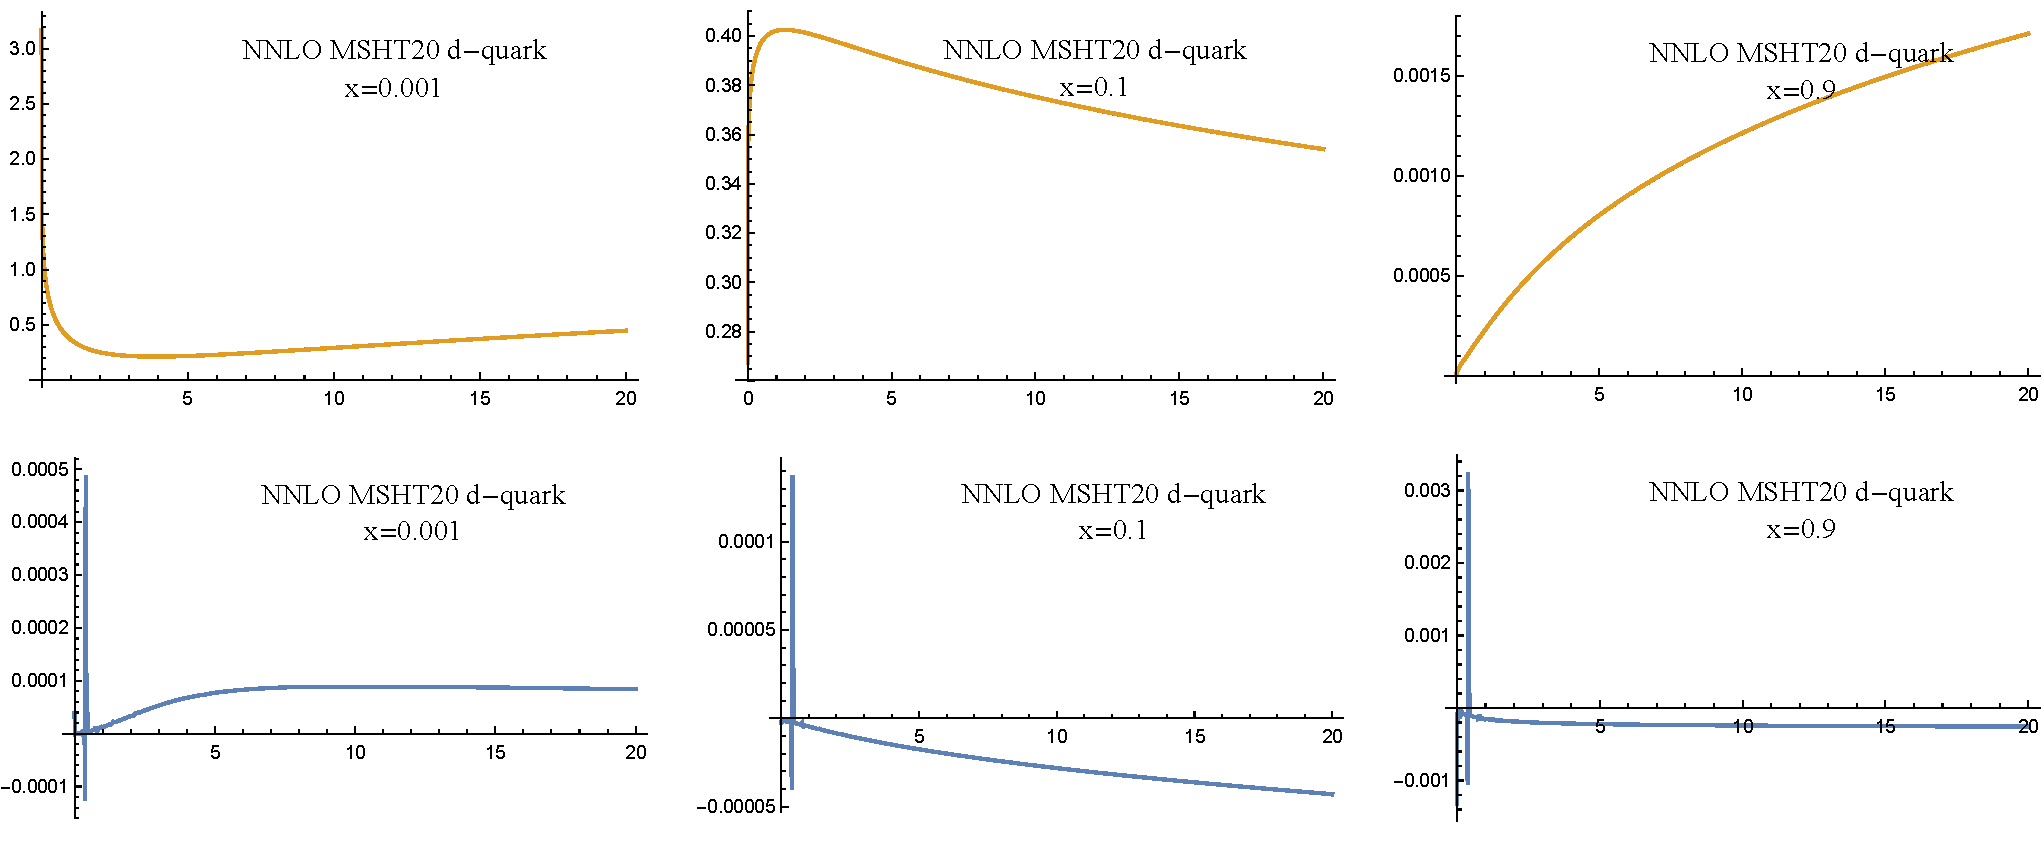
\includegraphics[width=\textwidth]{Figures/uTMDPDF_OPE.pdf}
\caption{\label{fig:OPE1} Example of convolution (vs.b). Upper row is the convolution. Lower row is the ratio of extraction vs. computaion. The peak in vicinity $b\sim 0.4$ is the quark threshold.}
\end{center}
\end{figure}


\textbf{Extra Notes:}
\begin{itemize}
\item Grid is computed by parallel do (if OMP is enabled).
\end{itemize}

\subsubsection{Technical notes}
\label{sec:technicalNote_1}

\begin{center}
\textbf{Convolution}
\end{center}

The convolution integral reads
\begin{eqnarray}
I(x)=\int_x^1 \frac{dz}{z}C(z)f\(\frac{x}{z}\)f_{NP}(x,z),
\end{eqnarray}
where the function $C(z)$ has a general form
\begin{eqnarray}
C(z)=C_0 \delta(1-z)+\(C_1(z)\)_++C_2(z).
\end{eqnarray}
Here the plus-distribution is undestood in the usual way
\begin{eqnarray}
\(C_1(z)\)_+=C_1(z)-\delta(1-z)\int_0^1 dy C_1(y)dy.
\end{eqnarray}
In NNLO coefficient function there are only possible two $(..)_+$ terms, $1/(1-z)$ and $\ln(1-z)/(1-z)$.

In order to simplify the integration we rewrite
\begin{eqnarray}
I(x)=\frac{1}{x}\int_x^1 dz C(z)\tilde f\(\frac{x}{z}\)f_{NP}(x,z),\qquad \tilde f(z)=zf(z).
\end{eqnarray}
Then the integral is split as
\begin{eqnarray}
I(x)=\frac{1}{x}\Big\{I_2(x)+C_0\tilde f\(x\)f_{NP}(x,1)+\tilde f\(x\)f_{NP}(x,1)\int_0^x dz C_1(z)\Big\},
\end{eqnarray}
where
\begin{eqnarray}
I_2(x)=\int_x^1 dz \Big[C_1(z)\(\tilde f\(\frac{x}{z}\)f_{NP}(x,z)-\tilde f\(x\)f_{NP}(x,1)\)+C_1(z)\tilde f\(\frac{x}{z}\)f_{NP}(x,z)\Big]
\end{eqnarray}
Presumably, the term $\sim C_0$ give the dominant contribution $w$, since it is $\sim 1$ whereas the other terms $\sim a_s$. Therefore, it serves as the estimation of the integral value, with respect to which the integration convergence is calculated. The convolution integral is evaluated by the G7K15 rule adaptively with given tolerance with respect to $w$. 

The integral $I$ is calculated in the procedure \texttt{Common\_lowScale50} and \texttt{Common\_lowScale5}, which is common for all twist-2 terms. The integral $I_2$ is calculated in the iterative procedures \texttt{MellinConvolutionVectorPart50} and \texttt{MellinConvolutionVectorPart5}, which is common for all twist-2 terms. 

\textbf{In the case of TMDFF} we have the coefficient function with the structure $C(z)/z^2$ (plus-distribution, $\delta$, etc, are multiplied by $1/z^2$), and collinear function $f(z)/z^2$. In this case it is convenient to rewrite
\begin{eqnarray}
I(x)=\int_x^1 \frac{dz}{z}\frac{C(z)}{z^2}\frac{f\(\frac{x}{z}\)}{(x/z)^2}f_{NP}(x,z)=\frac{1}{x^3}\int_x^1 dz C(z)\hat f\(\frac{x}{z}\)f_{NP}(x,z),\qquad \hat f(z)=zf(z).
\end{eqnarray}
Since the common-code calculates the integral PDF-like convolution, I divide by factor $1/x^2$ all output of the common-code.

\begin{center}
\textbf{Coefficient functions}
\end{center}

The coefficient function is spit to 6 terms.
\begin{eqnarray}
C_{q\ot q},\quad C_{q\ot g},\quad C_{g\ot q},\quad C_{g\ot g},\quad C_{q\ot \bar q},\quad C_{q\ot \bar q},\quad C_{q\ot q'},
\end{eqnarray}
where $C_{q\ot q}$ and $C_{q\ot \bar q}$ contain \textit{non-singlet} part only. The singlet contribution is given in $C_{q\ot q'}$. So, the convolution for a quark (e.g. $q=u$) reads
\begin{eqnarray}
F_u=C_{q\ot q}\otimes q_u+C_{q\ot g}\otimes q_g+C_{q\ot \bar q}\otimes q_{\bar u}+C_{q\ot q'}\otimes \sum_{f\in q,\bar q} q_f.
\end{eqnarray}
For gluon
\begin{eqnarray}
F_g=C_{g\ot g}\otimes q_g+C_{g\ot q}\otimes \sum_{f\in q,\bar q} q_f.
\end{eqnarray}

The kernels are split into regular, singular and $\delta$-parts, where singular contains $(\ln(1-x)/(1-x)))_+^n$ terms, $\delta$ contains only $\delta(1-x)$ terms, and regular is the rest. Singular and $\delta$-terms are present only for $C_{q\ot q}$ and $C_{g\ot g}$.

The regular part is decomposed further, into singular (but integrable) terms at $x\to0 $ and $x\to 1$, and the finite part. The singular terms are computed exactly, while the finite part is fitted to linear combination of several functions. The basis of fit is such that the expressions are exact for coefficients which do not contain PolyLog functions. These are NLO, leading log [at all orders], large-Nf [at all orders], and some others. The full basis for the regular part is
\begin{eqnarray}
&&\Big\{\underbrace{\ln \bar x,\ln^2\bar x,\ln^3\bar x,\ln^4\bar x,\ln^5\bar x,
\frac{1}{x},\frac{\ln x}{x},\frac{\ln^2x}{x},
\ln x,\ln^2x,\ln^3x,\ln^4x,\ln^5x,}_{\substack{\text{singular-integrable} \\ \text{exact}}}
\\\nn&&
\underbrace{1,x}_{\text{exact}},x\bar x ,
x\(\frac{\ln x}{1-x}+1\), \frac{x \ln^2x}{1-x}, \frac{x\ln^3x}{1-x},
x\ln x,x\ln^2x,x\ln^3x,x\ln^4x,
x\bar x\ln x,x\bar x\ln^2x,x\bar x\ln^3x,
\\\nn &&
\bar x\ln\bar x,\bar x\ln^2\bar x,\bar x\ln^3\bar x,
x\bar x\ln\bar x,x\bar x\ln^2\bar x,x\bar x\ln^3\bar x,
\ln x\ln\bar x,x\ln x\ln\bar x,x\bar x\ln x\ln\bar x,
\frac{\ln\bar x(1-x^2+2\ln x)}{1-x},
\frac{\bar x(\ln x+x)}{x}
\Big\}.
\end{eqnarray}
Decomposed in this basis the coefficient functions are very presice. The typical relative precision is $10^{-8}-10^{-10}$ \textit{for the finite part} (other terms are exact). The worst presicion happen at small $x\sim 10^{-5}$ for $g\ot g$ channel where relative precision is $\sim 10^{-5}-10^{-6}$.

Similar ansatz is used for uTMDFF, with some term removed (which are sensitive to small-x region). Precision in the case of TMDFF is slightly worse $10^{-6}-10^{-8}$. The worst precision is for N$^3$LO $q\to q'$ channel, where it is $\sim 10^{-4}-10^{-6}$. However, it is very good precision which guaranties about 10-12 presice digits for the physical convolution.

\begin{center}
\textbf{Computation of AS$[\mathcal{X}_0]$}
\end{center}

The function AS$\mathcal{X}_0$ is defined in [????.????] and reads
\begin{eqnarray}\label{def:AS_X0}
\text{AS}[\mathcal{X}_0[F]]&=&\alpha_s \Big\{P_1+\alpha_s\[P_2+\(C_1-P_1\)\otimes\(P_1-\beta_0\)\]
\\\nn &&+\alpha_s^2\Big[P_3+\(C_1-P_1\)\otimes\(P_2-\beta_1\)
+\(C_2-P_2\)\otimes\(P_1-2\beta_0\)
\\\nn &&-\(C_1-P_1\)\otimes\(P_1-\beta_0\)\otimes\(P_1-2\beta_0\)\Big]
+\mathcal{O}\(\alpha_s^3\)\Big\}\otimes f.
\end{eqnarray}
I could be obtained by computation of ordinary optimal small-b convolution with replacement of finite terms by $0$, and logarithm terms by $\mathbf{L}_b^k\to -k!$. Thus, the function can be computed as ordinary convolution with the coefficient function $X$ defined as (up to N$^3$LO)
\begin{eqnarray}
X=\frac{3}{4}C[\mathbf{L}_b=0]-\frac{2}{3}C[\mathbf{L}_b=1]-\frac{1}{12}C[\mathbf{L}_b=4].
\end{eqnarray}



\subsection{\texttt{\_OPE} modules (tw3)}
\label{TMD_OPE_tw3}

OPE modules compute the following convolution
\begin{eqnarray}\label{OPE:tw3:main}
[C\times T](x)&=&\int [dy] C_{\text{tw3}}(y_{1,2,3}),\mathbf{L})T\(y_{1,2,3},\mu_{\text{OPE}}\),
\end{eqnarray}
where $T$ is a twist-three function (qgq-correlator) and
\begin{eqnarray}
\mathbf{L}=\ln\(\frac{\mu^2_{\text{OPE}}b^2}{4e^{-2\gamma_E}}\).
\end{eqnarray}

\begin{tcolorbox}
\begin{center}
OPE modules are initialized automatically from the corresponding TMD module.
\end{center}
\end{tcolorbox}

\begin{tcolorbox}
\begin{center}
\red{
\textbf{Twist-3 convolution is not implemented yet. All function are placeholders. The only working order is NA.}}
\end{center}
\end{tcolorbox}

\subsubsection{Functions}

\begin{center}
\texttt{XX}=name of module (e.g. \texttt{uTMDPDF}, \texttt{uTMDFF}, etc.)
\\
\begin{tabular}{||p{5.5cm}||c||p{8.5cm}||}
\hline\hline
Entry &~~Type~~& Description
\\\hline
\texttt{XX\_OPE\_Initialize(file,prefix)} & subroutine & Initialize the module from INI-file. (common with tw2-part)
\\\hline
\texttt{XX\_tw3\_resetGrid()} & subroutine & Force recomputation of the grid. Only if griding is ON.
\\\hline
\texttt{XX\_OPE\_tw3\_testGrid()} & subroutine & Run the test of grid (see sec.\ref{sec:OPE:grid1}).  Only if griding is ON.
\\\hline
\texttt{XX\_OPE\_tw3\_SetPDFreplica(rep,h)} & subroutine & Switch the PDF replica to \texttt{rep}(int) for hadron \texttt{h} (int). Recompute the grid (if griding is ON). If the new replica is as before nothing is done.
\\\hline
\texttt{XX\_OPE\_tw3\_SetScaleVariation(c4)} & subroutine & Change the scale variation parameter $c_4$ (it enters the definition of $\mu_{\text{OPE}}$). Recompute the grid (if griding is ON). The parameter (real)\texttt{c4} is restricted to $0.1<c_4<10$.
\\\hline\hline
\texttt{XX\_OPE\_tw3\_convolution(x,b,h,G)} & dp\_real(-5:5) & Returns (\ref{OPE:tw3:main}) for (x,b)=((real)\texttt{x}, (real)\texttt{b}), and hadron number (int)\texttt{h}. In the case of \texttt{NA} returns 1. If grid is computed restore from the grid. The flag (T/F)\texttt{G} is optional. It indicates the inclusion of gluon into the result. Note, that if gluons were not included into the grid they are zero.
\\\hline\hline
\end{tabular}
\end{center}

\subsubsection{Model parameters.} 

The OPE is fully deterministic formula, but it contains the free scale, and often one implement $b^*$-modification. These parameters are written in \texttt{model}-module. Namely:
\begin{itemize}
\item \texttt{bSTAR(bT,x,y)} = is the function used instead of $b$ in  $\mathbf{L}$ in eqn.(\ref{OPE:tw2:main}).
\item \texttt{muOPE(bt,x,y,c4)} = is the function used for $\mu_{\text{OPE}}$.
\end{itemize}
In both cases, the variables $x$ and $y$ are defined as in eqn.(\ref{OPE:tw2:main}). The parameter $c_4$ is the scale variation parameter.

\subsubsection{Scale variation.} 

\textbf{Not implemented yet}

\subsubsection{Grid}
\label{sec:OPEtw3:grid1}

\textbf{Not implemented yet}

\subsection{Fourier to $k_T$ space}
\label{sec:Fourier_to_kt}

We define
\begin{eqnarray}
F(x,\vec k_T;\mu,\zeta)=\int \frac{d^2\vec b}{(2\pi)^2}F(x,\vec b;\mu,\zeta)e^{-i(\vec k_T \vec b)}.
\end{eqnarray}
Since all evaluated TMDs depends only on the modulus of $\vec b$, within the module we evaluate Hankel transformations. These transformations depends on the kind of TMD. Generally the integrals are
\begin{eqnarray}\label{kT-J0}
F(x,|\vec k_T|;\mu,\zeta)=\frac{M^{2n}}{n!}\int \frac{|b|d|\vec b|}{2\pi} \(\frac{|\vec  b|}{|k_T|}\)^{n} J_n(|\vec b||\vec k_T|) F(x,|\vec b|;\mu,\zeta),
\end{eqnarray}
where the parameter $M$ is the mass-scale (defined globally for all modules). The value of $n$ dependents on the type of the TMD distributions. Particularly, there are
\begin{itemize}
\item For \texttt{uTMDPDF}, \texttt{uTMDFF}
$$
n=0,\qquad F(x,|\vec k_T|;\mu,\zeta)=\int \frac{d|\vec b|}{2\pi}|\vec  b| J_0(|\vec b||\vec k_T|) F(x,|\vec b|;\mu,\zeta),
$$

\item For \texttt{SiversTMDPDF}, \texttt{BoerMuldersTMDPDF}, \texttt{wgtTMDPDF}
$$
n=1,\qquad F(x,|\vec k_T|;\mu,\zeta)=\frac{M^2}{k_T}\int \frac{d|\vec b|}{2\pi}|\vec  b|^2 J_1(|\vec b||\vec k_T|) F(x,|\vec b|;\mu,\zeta),
$$

\item For \texttt{lpTMDPDF}
$$
n=2,\qquad F(x,|\vec k_T|;\mu,\zeta)=\frac{M^4}{2k_T^2}\int \frac{d|\vec b|}{2\pi}|\vec  b|^3 J_2(|\vec b||\vec k_T|) F(x,|\vec b|;\mu,\zeta),
$$
\end{itemize}

\subsection{TMMD}
\label{sec:TMM}

In ref.[2402.01836] the following TMMs are defined
\begin{eqnarray}
\mathcal{G}_{n,n}[F]=\mathcal{G}[F]&=&\frac{1}{n!}\int_0^\infty db \mu \(\frac{\mu b}{2}\)^n J_{n+1}(\mu b)F(x,b)
\\
\mathcal{G}_{n+1,n}[F]=\mathcal{X}[F]&=&\frac{1}{2M^2n!}\int_0^\infty db \mu^3 \(\frac{\mu b}{2}\)^n \frac{(n+1)J_{n+1}(\mu b)-J_{n+3}(\mu b)}{n+2}F(x,b)
\\\nn
&=&
\frac{1}{2M^2n!}\int_0^\infty db \mu^3 \(\frac{\mu b}{2}\)^n \(J_{n+1}(\mu b)-\frac{J_{n+2}(\mu b)}{(\mu b)}\)F(x,b)
\end{eqnarray}
The correspond to the cut-integral over TMD and particular TMMs. The value of n is defined by the type of TMD (see sec.\ref{sec:Fourier_to_kt}).

\renewcommand{\arraystretch}{1.5}
\newpage


\section{\texttt{TMDs} module}
\label{TMDs}

The module \texttt{TMDs} joins the lower modules and performs the evaluation of various TMD distributions in the $\zeta$-prescription. Generally a TMD distribution is given by the expression
\begin{eqnarray}
F_f(x,b;\mu,\zeta)=R_f[b,(\mu,\zeta)\to(\mu_i,\zeta_{\mu_i})]\tilde F_f(x,b),
\end{eqnarray}
where $R$ is the TMD evolution kernel, $\tilde F$ is a TMD distribution at low scale. The scale $\mu_i$ is dependent on the evolution type, and could be out of use. Note, that \texttt{TMDs} initializes the lower modules automatically. Therefore, no special initializations should be done.

\begin{center}
List of available commands
\\
\begin{tabular}{||l|c|c|p{8cm}||}
\hline\hline
Command & ~~Type~~& ~~Sec.~~ & Short description
\\\hline
\texttt{TMDs{\_}Initialize(file,\blue{prefix})} & subrout. & - & Initialization of module. (string) \texttt{file} is the name of \texttt{constants-file}, which contains initialization information. (string)\texttt{prefix} is appended to \texttt{file} if provided.
\\\hline
\texttt{TMDs\_SetScaleVariations(c1,c3)} & subrout. & \ref{TMDs:c123} & Set new values for the scale-variation constants.
\\\hline\hline
\texttt{uTMDPDF{\_}5(x,b,mu,zeta,h)} & (real*8(-5:5)) &\ref{TMDs:TMDs} & Unpolarized TMD PDF (gluon term undefined)
\\\hline
\texttt{uTMDPDF{\_}50(x,b,mu,zeta,h)} & (real*8(-5:5)) &\ref{TMDs:TMDs} & Unpolarized TMD PDF (gluon term defined)
\\\hline
\texttt{uTMDFF{\_}5(x,b,mu,zeta,h)} & (real*8(-5:5)) &\ref{TMDs:TMDs} & Unpolarized TMD FF (gluon term undefined)
\\\hline
\texttt{uTMDFF{\_}50(x,b,mu,zeta,h)} & (real*8(-5:5)) &\ref{TMDs:TMDs} & Unpolarized TMD FF (gluon term defined)
\\\hline
\texttt{lpTMDPDF{\_}50(x,b,mu,zeta,h)} & (real*8(-5:5)) &\ref{TMDs:TMDs} & Linearly polarized gluon TMD PDF (quarks are zero)
\\\hline
\texttt{SiversTMDPDF{\_}5(x,b,mu,zeta,h)} & (real*8(-5:5)) &\ref{TMDs:TMDs} & Sivers TMD PDF (gluon term undefined)
\\\hline
\texttt{SiversTMDPDF{\_}50(x,b,mu,zeta,h)} & (real*8(-5:5)) &\ref{TMDs:TMDs} & Sivers TMD PDF (gluon term defined)
\\\hline
\texttt{wgtTMDPDF{\_}5(x,b,mu,zeta,h)} & (real*8(-5:5)) &\ref{TMDs:TMDs} & worm-gear T TMD PDF (gluon term undefined)
\\\hline
\texttt{wgtTMDPDF{\_}50(x,b,mu,zeta,h)} & (real*8(-5:5)) &\ref{TMDs:TMDs} & worm-gear T TMD PDF (gluon term defined)
\\\hline\hline
\texttt{uTMDPDF{\_}5(x,b,h)} & (real*8(-5:5)) &\ref{TMDs:TMDs} & Unpolarized TMD PDF at optimal line (gluon term undefined)
\\\hline
\texttt{uTMDPDF{\_}50(x,b,,h)} & (real*8(-5:5)) &\ref{TMDs:TMDs} & Unpolarized TMD PDF at optimal line (gluon term defined)
\\\hline
\texttt{uTMDFF{\_}5(x,b,h)} & (real*8(-5:5)) &\ref{TMDs:TMDs} & Unpolarized TMD FF at optimal line(gluon term undefined)
\\\hline
\texttt{uTMDFF{\_}50(x,b,h)} & (real*8(-5:5)) &\ref{TMDs:TMDs} & Unpolarized TMD FF at optimal line (gluon term defined)
\\\hline
\texttt{lpTMDPDF{\_}50(x,b,,h)} & (real*8(-5:5)) &\ref{TMDs:TMDs} & Linearly polarized gluon TMD PDF at optimal line (quarks are zero)
\\\hline
\texttt{SiversTMDPDF{\_}5(x,b,h)} & (real*8(-5:5)) &\ref{TMDs:TMDs} & Sivers TMD PDF at optimal line (gluon term undefined)
\\\hline
\texttt{SiversTMDPDF{\_}50(x,b,,h)} & (real*8(-5:5)) &\ref{TMDs:TMDs} & Sivers TMD PDF at optimal line (gluon term defined)
\\\hline
\texttt{wgtTMDPDF{\_}5(x,b,h)} & (real*8(-5:5)) &\ref{TMDs:TMDs} & Worm gear T TMD PDF at optimal line (gluon term undefined)
\\\hline
\texttt{wgtTMDPDF{\_}50(x,b,,h)} & (real*8(-5:5)) &\ref{TMDs:TMDs} & Worm gear T TMD PDF at optimal line (gluon term defined)
\\\hline
\texttt{BoerMuldersTMDPDF{\_}5(x,b,h)} & (real*8(-5:5)) &\ref{TMDs:TMDs} & Sivers TMD PDF at optimal line (gluon term undefined)
\\\hline
\texttt{BoerMuldersTMDPDF{\_}50(x,b,,h)} & (real*8(-5:5)) &\ref{TMDs:TMDs} & Sivers TMD PDF at optimal line (gluon term defined)
\\\hline\hline
\texttt{uPDF{\_}uPDF(x1,x2,b,mu,zeta,h1,h2)} & (real*8(-5:5)) &\ref{TMDs:products} &  Product of Unpolarized TMD PDF $f_{q\ot h_1}(x_1)f_{\bar q\ot h_1}$ at the same scale (gluon term undefined)
\\
\hline\hline
\end{tabular}
\\
~
\\
List of functions which must be provided by a model code
\\
\begin{tabular}{||l|l||}
\hline\hline
Input &  Short description
\\\hline
\texttt{mu{\_}LOW(b)} & The value of $\mu_i$ used in the evolutions of type 1 and 2 (improved $\mathcal{D}$ and $\gamma$). See \cite{Scimemi:2018xaf}.
\\\hline
\texttt{mu0(b)}& The value of $\mu_0$ used in the evolution of type 1 (improved $\mathcal{D}$). See \cite{Scimemi:2018xaf}.
\\
\hline\hline
\end{tabular}
\end{center}

\subsection{Definition of low-scales}
\label{TMDs:mus}

The low scales $\mu_i$ and $\mu_0$ are defined in the functions \texttt{mu{\_}LOW(bt)} and \texttt{mu0(bt)} which can be found in the end of \texttt{TMDs.f90} code. Modify it if needed.



\subsection{Evaluating TMDs}
\label{TMDs:TMDs}

The expression for unpolarized TMD PDF is obtained by the functions

(real*8(-5:5))\texttt{uTMDPDF{\_}5(x,b,mu,zeta,h)}

where 
\begin{itemize}
\item [\texttt{x}] (real*8) Bjorken-$x$ ($0<x<1$)
\item [\texttt{b}] (real*8) Transverse distance ($b>0$) in GeV
\item [\texttt{mu}] (real*8) The scale $\mu_f$ in GeV. Typically, $\mu_f=Q$.
\item [\texttt{zeta}] (real*8) The scale $\zeta_f$ in GeV$^2$. Typically, $\zeta_f=Q^2$.
\item [\texttt{h}] (integer) The hadron type. If $h<0$, the hadron is anti-hadron.
\end{itemize}
This function return the vector real*8(-5:5) for $\bar b, \bar c, \bar s,\bar u,\bar d ,?,d,u,s, c, b$.

\begin{itemize}
\item Gluon contribution in \texttt{uTMDPDF{\_}5} is undefined, but taken into account in the mixing contribution. The point is that evaluation of gluons slow down the procedure approximately by $40\%$, and often is not needed. To calculate the full flavor vector with the gluon TMD, call \texttt{uTMDPDF{\_}50(x,b,mu,zeta,h)}, where all arguments defined in the same way.

\item The other TMDs, such as unpolarized TMDFF, transversity, etc. are obtained by similar function see the table in the beginning of the section.

\item Each function has version without parameters \texttt{mu} and \texttt{zeta}. It corresponds to the evaluation of a TMS at optimal line \cite{Scimemi:2018xaf}. Practically, it just transfers the outcome of corresponding TMD module, e.g.module \texttt{uTMDPDF}, see sec.\ref{uTMDPDF}.

\item For $h<0$ the quark-distributions are replaced by anti-quark distributions and vice versa. I.e. $F(-h)=F(h)(5:-5:-1)$ [it is done in TMDs-Modules]
\end{itemize}

\subsection{Products of TMDs}
\label{TMDs:products}

The the evaluation of majority of cross-sections one needs the product of two TMDs at the same scale. There are set of functions which return these products. They are slightly faster then just evaluation and multiplication, due to the flavor blindness of the TMD evolution. The function have common interface

(real*8(-5:5)) \texttt{uPDF{\_}uPDF(x1,x2,b,mu,zeta,h1,h2)}

where
\begin{itemize}
\item [\texttt{x1,x2}] (real*8) Bjorken-$x$'s ($0<x<1$)
\item [\texttt{b}] (real*8) Transverse distance ($b>0$) in GeV
\item [\texttt{mu}] (real*8) The scale $\mu_f$ in GeV. Typically, $\mu_f=Q$.
\item [\texttt{zeta}] (real*8) The scale $\zeta_f$ in GeV$^2$. Typically, $\zeta_f=Q^2$.
\item [\texttt{h1,h2}] (integer) The hadron's types.
\end{itemize}
The function return a product of the form $F_{f_1\ot h_1}(x_1,b;\mu,\zeta)F_{f_2\ot h_2}(x_2,b;\mu,\zeta)$, where $f_{1,2}$ and the type of TMDs depend on the function.



\subsection{Theoretical uncertainties}
\label{TMDs:c123}

\texttt{TMDs\_SetScaleVariations(c1,c3,c4)} changes the scale multiplicative factors $c_i$ (see \cite{Scimemi:2018xaf}, sec.6). The default set of arguments is (1,1,1), i.e. the scales as they given in corresponding functions. This subroutine changes $c1$ and $c3$ constants and call corresponding subroutines for variation of $c4$ in TMD defining packages. Note, that in some types of evolution particular variations absent.

\newpage

\section{\texttt{TMDF} module}
\label{TMDF}


This module evaluates the structure functions, that are universally defined as
\begin{eqnarray}\label{TMDF:F}
F(Q^2,q_T,x_1,x_2,\mu,\zeta_1,\zeta_2)=\int_0^\infty \frac{bdb}{2}b^n J_n(bq_T)\sum_{ff'} z_{ff'}(Q^2) F_1^f(x_1,b;\mu,\zeta_1)F_2^{f'}(x_2,b;\mu,\zeta_2),
\end{eqnarray}
where
\begin{itemize}
\item $Q^2$ is hard scale.
\item $q_T$ is transverse momentum in the factorization frame. It coincides with measured $q_T$ in center-mass frame for DY, but $q_T\sim p_T/z$ for SIDIS.
\item $x_1$ and $x_2$ are parts of collinear parton momenta. I.e. for DY $x_{1,2}\simeq Qe^{\pm y}/\sqrt{s}$, while for SIDIS $x_2\sim z$. It can also obtain power correction, ala Nachmann variables.
\item $\mu$ is the hard factorization scale $\mu \sim Q$
\item $\zeta_{1,2}$ are rapidity factorization scales. In the standard factorization scheme $\zeta_1\zeta_2=Q^4$. It can also be modified by power corrections.
\item $f,f'$ are parton flavors.
\item $z_{ff'}$ is the process related function. E.g. for photon DY on $p+\bar p$, $z_{ff'}=\delta_{ff'}|e_f|^2.$
\item $n$ The order of Bessel transformation is defined by structure function. E.g. for unpolarized DY $n=1$. For SSA's $n=1$. In general for angular modulation $\sim \cos (n\theta)$.
\item $F_{1,2}^f$ TMD distribution (PDF or FF) of necessary polarization and flavor.
\end{itemize}
Some structure functions are multiplied by a constant with mass dimension (e.g. Sivers asymmetry). This constant (called global mass scale = $M$) is defined globally in the constants file.


\begin{center}
List of available commands
\\
\begin{tabular}{||l|c|c|p{8cm}||}
\hline\hline
Command & ~~Type~~& ~~Sec.~~ & Short description
\\\hline
\texttt{TMDF{\_}Initialize(file,\blue{prefix})} & subrout. & \ref{TMDF:init} & Initialization of module. (string) \texttt{file} is the name of \texttt{constants-file}, which contains initialization information. (string)\texttt{prefix} is appended to \texttt{file} if provided.
\\\hline
\texttt{TMDF\_ShowStatistic())} & subrout. & -- & Print current statistic on the number of calls.
\\\hline
\texttt{TMDF\_ResetCounters()} & subrout. & -- & Reset intrinsic counters. E.g.release convergenceISlost state.
\\\hline
\texttt{TMDF{\_}F(Q2,qT,x1,x2,mu,zeta1,zeta2,N)} & (real*8) &\ref{TMDF:TMDF} & Evaluates the structure function
\\\hline\hline
\end{tabular}
\end{center}

\subsection{Initialization}
\label{TMDF:init}

Prior the usage module is to be initialized (once per run) by

\texttt{call TMDF{\_}Initialize(file)}

It reads \texttt{constants-file} and initialize it-self accordingly.

\subsection{Evaluating Structure functions}
\label{TMDF:TMDF}

The value of the structure function is obtained by

(real*8)\texttt{TMDF{\_}F(Q2,qT,x1,x2,mu,zeta1,zeta2,N)}

where 
\begin{itemize}
\item [\texttt{Q2}] (real*8) hard scale in GeV$^2$.
\item [\texttt{qT}] (real*8) modulus of transverse momentum in the factorization frame in GeV, $q_T>0$
\item [\texttt{x1}] (real*8) $x$ passed to the first TMD distribution  ($0<x1<1$)
\item [\texttt{x2}] (real*8) $x$ passed to the first TMD distribution ($0<x2<1$)
\item [\texttt{mu}] (real*8) The hard scale $\mu$ in GeV. Typically, $\mu=Q$.
\item [\texttt{zeta1}] (real*8) The scale $\zeta_f$ in GeV$^2$ for the first TMD distribution. Typically, $\zeta_f=Q^2$.
\item [\texttt{zeta2}] (real*8) The scale $\zeta_f$ in GeV$^2$ for the second TMD distribution. Typically, $\zeta_f=Q^2$.
\item [\texttt{N}] (integer) The number of process.
\end{itemize}
The function returns the value of 
\begin{eqnarray}
F^N(Q^2,q_T,x_1,x_2,\mu,\zeta_1,\zeta_2)=\int_0^\infty \frac{bdb}{2}b^n J_n(bq_T)\sum_{ff'} z^N_{ff'}(Q^2) F_1^f(x_1,b;\mu,\zeta_1)F_2^{f'}(x_2,b;\mu,\zeta_2).
\end{eqnarray}
The parameter $n$ depends on the argument \texttt{N} and uniformly defined as 
\begin{eqnarray*}
n=0 &\qquad\qquad& \text{for \texttt{N}}<10000
\\
n=1 &\qquad\qquad& \text{for \texttt{N}}\in[10000,20000]
\\
n=2 &\qquad\qquad& \text{for \texttt{N}}\in[20000,30000]
\\
n=3 &\qquad\qquad& \text{for \texttt{N}}>30000
\end{eqnarray*}
The particular values of $z_{ff'}$ and $F_{1,2}$ are given in the following table. User function can be implemented by code modification.

\textbf{Notes on the integral evaluation:}
\begin{itemize}
\item The integral is uniformly set to 0 for $q_T<10^{-7}$.
\item The integrand is uniformly set to 0 for $b>10^{3}$.
\item If for any element of evaluation (including TMD evolution factors and convolution integrals, and the integral of the structure function it-self) obtained divergent value. The trigger is set to ON. In this case, the integral returns uniformly large value $10^{100}$ for all integrals without evaluation. The trigger is reset by new values of NP parameters. It is done in order to cut the improper values of NP parameters in the fastest possible way, which speed up fitting procedures.
\item The Fourier is made by Ogata quadrature, which is double exponential quadrature. I.e.
\begin{eqnarray}
\int_0^\infty \frac{bdb}{2} b^n I(b) J_n(q_Tb)\simeq \frac{1}{q_T^{n+2}}\sum_{k=1}^\infty \tilde \omega_{nk} b_{nk}^{n+1} I\(\frac{b_{nk}}{q_T}\),
\end{eqnarray}
where
$$
b_{nk}=\frac{\psi(\tilde h \tilde \xi_{nk})}{\tilde h}=\tilde \xi_{nk} \tanh(\frac{\pi}{2}\sinh(\tilde h \tilde \xi_{nk}))
$$
$$
\tilde \omega_{nk}=\frac{J_n(\tilde b_{nk})}{\tilde\xi_{nk} J^2_{n+1}(\tilde \xi_{nk})}\psi'(\tilde h \tilde \xi_{nk})
$$
Here, $\tilde \xi_{nk}$ is $k$'th zero of $J_n(x)$ function. Note, that $\tilde h=h/\pi$ in the original Ogata's notation.
\item The convergence properties of the quadrature essentially depends on $h$. I have found that $h\sim q_T$. For accurate evolution of integrals at different values of $q_T$ I set $h=h_0 s$, where $s$ is defined for intervals of $q_T$.
\item The sum over $k$ is restricted by $N_{\text{max}}$ where $N_{\text{max}}$ is hard coded number, $N_{\text{max}}=200$. 
\item The sum over $k$ is evaluated until the sum of absolute values of last four terms is less then \textit{tolerance}. If $M>N_{\text{max}}$ the integral declared divergent, and the trigger is set to ON.
\end{itemize}

\begin{tcolorbox}
\begin{center}
\textbf{WARNING!}
\\
The error for Ogata quadrature is defined by parameters $h$ and $M$(number of terms in the sum over $k$). In the parameter $M$ quadrature is double-exponential, i.e. converges fast as $M$ approaches $N_{\text{max}}$. And the convergence of the sum can be simply checked. In the parameter $h$ the quadrature is quadratic (the convergence is rather poor). The convergence to the true value of integral is very expensive especially at large $q_T$ (it requires the complete reevaluation of integral at all nodes). Unfortunately, $N_{\text{max}}\sim h^{-1}$, and has to find the balance value for $h$. In principle, TMD functions decays rather fast, and suggested default value $h=0.005$ is trustful. \textbf{Nonetheless, we suggest to test other values (*/2) of $h$ to validate the obtained values in your model.}

The adaptive check of convergence will implemented in the future versions.
\end{center}
\end{tcolorbox}

\subsection{Enumeration of structure functions}
\label{TMDF:enum}

\renewcommand{\arraystretch}{2.5}
\begin{center}
List of enumeration of structures functions
\\
\texttt{N}$<$10000
\\
\begin{longtable}{||l|p{5cm}|c|c||p{7cm}|c|c||}
\hline\hline
\texttt{N} & ~~$z_{ff'}$~~& ~~$F_1$~~ & ~~$F_2$~~&  Short description & Gluon & LP/KPC
\\\hline
0 &  &  &  &  & &
\\
9999 & -- & -- & -- & Test cases (see \ref{TMDF:tests}) & no & LP/KPC
\\
9998 &  &  &  &  & &
\\\hline
1 & $\delta_{\bar f f'}|e_f|^2$ & $f_1$ & $f_1$ & (unpol.)$h_1+h_2\to\gamma$ & no & LP/KPC
\\\hline
2 & $\Ds\delta_{\bar f f'}\frac{(1-2|ef|s_w^2)^2-4e_f^2s_w^4}{8s_w^2c_w^2}$ & $f_1$ & $f_1$ & (unpol.)$h_1+h_2\to Z$ & no & LP/KPC
\\\hline
3 & $\Ds\delta_{\bar f f'}\frac{z_{ll'}z_{ff'}}{\alpha_{\text{em}}^2}$ given in (2.8) of \cite{Scimemi:2017etj} & $f_1$ & $f_1$ & (unpol.)$h_1+h_2\to Z+\gamma$ & no & LP/KPC
\\\hline
4 & $\Ds \frac{1}{4s_w^2}\frac{|V_{f f'}|^2}{4s_w^2}\frac{Q^4}{(Q^2-M_W^2)^2+\Gamma_W^2M_W^2}$ & $f_1$ & $f_1$ & (unpol.)$h_1+h_2\to W^+$ & no & LP/KPC
\\\hline
5 & $\Ds \frac{1}{4s_w^2}\frac{|V_{f f'}|^2}{4s_w^2}\frac{Q^4}{(Q^2-M_W^2)^2+\Gamma_W^2M_W^2}$ & $f_1$ & $f_1$ & (unpol.)$h_1+h_2\to W^-$ & no & LP/KPC
\\\hline
6 & $\Ds \frac{1}{4s_w^2}\frac{|V_{f f'}|^2}{4s_w^2}\frac{Q^4}{(Q^2-M_W^2)^2+\Gamma_W^2M_W^2}$ & $f_1$ & $f_1$ & (unpol.)$h_1+h_2\to W^\pm$ & no & LP/KPC
\\\hline
7 & $\Ds \frac{|V_{f f'}|^2}{4s_w^2}$  & $f_1$ & $f_1$ & (unpol.)$h_1+h_2\to W^+$ (for narrow-width approx.) & no & LP/KPC
\\\hline
8 & $\Ds \frac{|V_{f f'}|^2}{4s_w^2}$  & $f_1$ & $f_1$ & (unpol.)$h_1+h_2\to W^-$ (for narrow-width approx.) & no & LP/KPC
\\\hline
9 & $\Ds \frac{|V_{f f'}|^2}{4s_w^2}$  & $f_1$ & $f_1$ & (unpol.)$h_1+h_2\to W^\pm$ (for narrow-width approx.) & no & LP/KPC
\\\hline
10 & $\Ds f_g(x_1)f_g(x_2)+h^\perp_{1}(x_1)h^\perp_{1}(x_2)$ & - & - & (unpol.)$h_1+h_2\to H$ Elementary Higgs production & yes & LP/KPC
\\\hline
11 & $\Ds f_g(x_1)f_g(x_2)$ & $f_1$ & $f_{1}$ & (unpol.)$h_1+h_2\to H$ Elementary Higgs production. Only unpol.TMDPDF term & yes & LP/KPC
\\\hline
12 & $\Ds h^\perp_{1g}(x_1)h^\perp_{1g}(x_2)$ & $h^\perp_{1}$ & $h^\perp_{1}$ & (unpol.)$h_1+h_2\to H$ Elementary Higgs production. Only linearly pol.TMDPDF term & yes & LP/KPC
\\\hline
101 & $\Ds R^{Cu}_{\bar f f'}e_f e_{f'} $ see (3.1) of \cite{Scimemi:2017etj} & $f_1$ & $f^{Cu}_1$ & (unpol.)$h_1+Cu\to \gamma$ where the isostructure of Cu is simulated from $hadron=1$, (used to describe E288 experiment) & no & LP/KPC
\\\hline
102 & $\Ds R^{^2H}_{\bar f f'}e_f e_{f'} $ see (3.1) of \cite{Scimemi:2017etj} with $Z=1$ and $A=2$ & $f_1$ & $f^{^2H}_1$ & (unpol.)$h_1+^2H\to \gamma$ where thes isostructure of $^2H$  is simulated from $hadron=1$, used to describe E772 experiment& no & LP/KPC
\\\hline
103 & $\Ds R^{^W}_{f f'}e_f e_{f'} $ see (3.1) of \cite{Scimemi:2017etj} with $Z=74$ and $A=183$ & $f_1$ & $f^{W}_1$ & (unpol.)$h_1+W\to \gamma$, where the  isostructure of $W$(tungsten) is simulated from $hadron=1$, used to describe E537 experiment& no & LP/KPC
\\\hline \hline
2001 & $\delta_{ff'}|e_f|^2$~~&$f^p_1$ & $d^{h_1}_1$ & (unpol)$p+\gamma\to h_1$ & no & LP
\\\hline
200N & $\delta_{ff'}|e_f|^2$~~&$f^p_1$ & $d^{h_N}_1$ & (unpol)$p+\gamma\to h_N$, for $N=\{1,...,9\}$ (including case 2001) & no & LP
\\\hline \hline
2011 & $\delta_{ff'}|e_f|^2$~~&$f^{d}_1$ & $d^{h_1}_1$ & (unpol)$d+\gamma\to h_1$. Here, d is isoscalar target $(p+n)/2$. & no & LP
\\\hline
201N & $\delta_{ff'}|e_f|^2$~~&$f^{d}_1$ & $d^{h_N}_1$ & (unpol)$d+\gamma\to h_N$, for $N=\{1,...,9\}$ (including case 2011). Here, d is isoscalar target $(p+n)/2$. & no & LP
\\\hline \hline
2021 & $\delta_{f\bar f'}|e_f|^2$~~&$f^p_1$ & $d^{\bar h_1}_1$ & (unpol)$p+\gamma\to \bar h_1$ & no & LP
\\\hline
202N & $\delta_{f\bar f'}|e_f|^2$~~&$f^p_1$ & $d^{\bar h_N}_1$ & (unpol)$p+\gamma\to \bar h_N$, for $N=\{1,...,9\}$ (including case 2021) & no & LP
\\\hline \hline
2031 & $\delta_{f\bar f'}|e_f|^2$~~&$f^{d}_1$ & $d^{\bar h_1}_1$ & (unpol)$d+\gamma\to \bar h_1$. Here, d is isoscalar target $(p+n)/2$. & no & LP
\\\hline
203N & $\delta_{f\bar f'}|e_f|^2$~~&$f^{d}_1$ & $d^{\bar h_N}_1$ & (unpol)$d+\gamma\to \bar h_N$, for $N=\{1,...,9\}$ ( including case 2031). Here, d is isoscalar target $(p+n)/2$. & no & LP
\\\hline \hline
204N & $\delta_{ff'}|e_f|^2$~~&$f^n_1$ & $d^{h_N}_1$ & (unpol)$n+\gamma\to h_N$, for $N=\{1,...,9\}$. n is neutron target $n=p(u\leftrightarrow d)$ & no & LP
\\\hline
205N & $\delta_{ff'}|e_f|^2$~~&$f^{n}_1$ & $d^{h_N}_1$ & (unpol)$n+\gamma\to \bar h_N$, for $N=\{1,...,9\}$. n is neutron target $n=p(u\leftrightarrow d)$. & no & LP
\\\hline \hline
2101 & $\delta_{ff'}|e_f|^2$~~&$f^p_1$ & $d^{h_{1+2}}_1$ & (unpol)$p+\gamma\to h_{1+2}$, where $h_{1+2}=h_1+h_2$ & no & LP
\\\hline
2102 & $\delta_{ff'}|e_f|^2$~~&$f^p_1$ & $d^{h_{1+2+3}}_1$ & (unpol)$p+\gamma\to h_{1+2+3}$, where $h_{1+2+3}=h_1+h_2+h_3$ & no & LP
\\\hline
2103 & $\delta_{ff'}|e_f|^2$~~&$f^d_1$ & $d^{h_{1+2}}_1$ & (unpol)$d+\gamma\to h_{1+2}$, where $h_{1+2}=h_1+h_2$ and d is isoscalar target $(p+n)/2$. & no & LP
\\\hline
2104 & $\delta_{ff'}|e_f|^2$~~&$f^d_1$ & $d^{h_{1+2+3}}_1$ & (unpol)$d+\gamma\to h_{1+2+3}$, where $h_{1+2+3}=h_1+h_2+h_3$ and d is isoscalar target $(p+n)/2$. & no & LP
\\\hline
2105 & $\delta_{ff'}|e_f|^2$~~&$f^n_1$ & $d^{h_{1+2}}_1$ & (unpol)$n+\gamma\to h_{1+2}$, where $h_{1+2}=h_1+h_2$ and n is neutron target $n=p(u\leftrightarrow d)$. & no & LP
\\\hline
2106 & $\delta_{ff'}|e_f|^2$~~&$f^n_1$ & $d^{h_{1+2+3}}_1$ & (unpol)$n+\gamma\to h_{1+2+3}$, where $h_{1+2+3}=h_1+h_2+h_3$ and n is neutron target $n=p(u\leftrightarrow d)$. & no & LP
\\\hline
2111 & $\delta_{f\bar f'}|e_f|^2$~~&$f^p_1$ & $d^{h_{1+2}}_1$ & (unpol)$p+\gamma\to \bar h_{1+2}$, where $h_{1+2}=h_1+h_2$ & no & LP
\\\hline
2112 & $\delta_{f\bar f'}|e_f|^2$~~&$f^p_1$ & $d^{h_{1+2+3}}_1$ & (unpol)$p+\gamma\to \bar h_{1+2+3}$, where $h_{1+2+3}=h_1+h_2+h_3$ & no & LP
\\\hline
2113 & $\delta_{f\bar f'}|e_f|^2$~~&$f^d_1$ & $d^{h_{1+2}}_1$ & (unpol)$d+\gamma\to \bar h_{1+2}$, where $h_{1+2}=h_1+h_2$ and d is isoscalar target $(p+n)/2$. & no & LP
\\\hline
2114 & $\delta_{f\bar f'}|e_f|^2$~~&$f^d_1$ & $d^{h_{1+2+3}}_1$ & (unpol)$d+\gamma\to \bar h_{1+2+3}$, where $h_{1+2+3}=h_1+h_2+h_3$ and d is isoscalar target $(p+n)/2$. & no & LP
\\\hline
2115 & $\delta_{f\bar f'}|e_f|^2$~~&$f^n_1$ & $d^{h_{1+2}}_1$ & (unpol)$n+\gamma\to \bar h_{1+2}$, where $h_{1+2}=h_1+h_2$ and n is neutron target $n=p(u\leftrightarrow d)$. & no & LP
\\\hline
2116 & $\delta_{f\bar f'}|e_f|^2$~~&$f^n_1$ & $d^{h_{1+2+3}}_1$ & (unpol)$n+\gamma\to \bar h_{1+2+3}$, where $h_{1+2+3}=h_1+h_2+h_3$ and n is neutron target $n=p(u\leftrightarrow d)$. & no & LP
\\\hline\hline
\end{longtable}

10000$\leqslant$\texttt{N}$<$20000
\\
\begin{longtable}{||l|p{6cm}|c|c||p{7cm}|c||}
\hline\hline
\texttt{N} & ~~$z_{ff'}$~~& ~~$F_1$~~ & ~~$F_2$~~&  Short description & Gluon req. 
\\\hline
10000 &  &  &  &  & 
\\
19999 & -- & -- & -- & Test cases (see \ref{TMDF:tests}) & no
\\
19998 &  &  &  &  & 
\\\hline\hline
10001 & $-M\delta_{\bar f f'}|e_f|^2$ & $-(f_{1T}^\perp)^p$ & $f_1$ & (Sivers)$h_1^{\uparrow}+h_2\to\gamma$ & no
\\\hline
10003 & $-M\Ds\delta_{\bar f f'}\frac{z_{ll'}z_{ff'}}{\alpha_{\text{em}}^2}$ given in (2.8) of \cite{Scimemi:2017etj} & $-(f_{1T}^\perp)^p$ & $f_1$ & (Sivers)$h_1^{\uparrow}+h_2\to Z+\gamma$ & no
\\\hline
10004 & $-M\Ds \frac{1}{4s_w^2}\frac{|V_{f f'}|^2}{4s_w^2}\frac{Q^4}{(Q^2-M_W^2)^2+\Gamma_W^2M_W^2}$ & $-(f_{1T}^\perp)^p$ & $f_1$ & (Sivers)$h_1^{\uparrow}+h_2\to W^+$ & no
\\\hline
10008 & $-M\Ds \frac{1}{4s_w^2}\frac{|V_{f f'}|^2}{4s_w^2}\frac{Q^4}{(Q^2-M_W^2)^2+\Gamma_W^2M_W^2}$ & $-(f_{1T}^\perp)^p$ & $f_1$ & (Sivers)$h_1^{\uparrow}+h_2\to W^-$ & no
\\\hline
10011 & $+M\delta_{\bar f f'}|e_f|^2$ & $f^h_1$ & $-(f_{1T}^\perp)^{p}$ & (Sivers)$h+p^\uparrow\to\gamma$ (with $h=2$) & no
\\\hline \hline
12001 & $-M\delta_{ff'}|e_f|^2$~~&$(f_{1T}^\perp)^p$ & $d^{h_1}_1$ & (Sivers)$p^{\uparrow}+\gamma\to h_1$ & no
\\\hline
1200N & $-M\delta_{ff'}|e_f|^2$~~&$(f_{1T}^\perp)^p$ & $d^{h_N}_1$ & (Sivers)$p^{\uparrow}+\gamma\to h_N$, for $N=\{1,...,9\}$ (including case 12001) & no
\\\hline \hline
12011 & $-M\delta_{ff'}|e_f|^2$~~&$(f_{1T}^\perp)^{d}$ & $d^{h_1}_1$ & (Sivers)$d^{\uparrow}+\gamma\to h_1$. Here, d is isoscalar target $(p+n)/2$. & no
\\\hline
1201N & $-M\delta_{ff'}|e_f|^2$~~&$(f_{1T}^\perp)^{d}$ & $d^{h_N}_1$ & (Sivers)$d^{\uparrow}+\gamma\to h_N$, for $N=\{1,...,9\}$ (including case 12011). Here, d is isoscalar target $(p+n)/2$. & no
\\\hline \hline
12021 & $-M\delta_{f\bar f'}|e_f|^2$~~&$(f_{1T}^\perp)^p$ & $d^{\bar h_1}_1$ & (Sivers)$p^{\uparrow}+\gamma\to \bar h_1$ & no
\\\hline
1202N & $-M\delta_{f\bar f'}|e_f|^2$~~&$(f_{1T}^\perp)^p$ & $d^{\bar h_N}_1$ & (Sivers)$p^{\uparrow}+\gamma\to \bar h_N$, for $N=\{1,...,9\}$ (including case 12021) & no
\\\hline \hline
12031 & $-M\delta_{f\bar f'}|e_f|^2$~~&$(f_{1T}^\perp)^{d}$ & $d^{\bar h_1}_1$ & (Sivers)$d^{\uparrow}+\gamma\to \bar h_1$. Here, d is isoscalar target $(p+n)/2$. & no
\\\hline
1203N & $-M\delta_{f\bar f'}|e_f|^2$~~&$(f_{1T}^\perp)^{d}$ & $d^{\bar h_N}_1$ & (Sivers)$d^{\uparrow}+\gamma\to \bar h_N$, for $N=\{1,...,9\}$ (including case 12031). Here, d is isoscalar target $(p+n)/2$. & no
\\\hline\hline
1204N & $-M\delta_{ff'}|e_f|^2$~~&$(f_{1T}^\perp)^d$ & $d^{h_N}_1$ & (Sivers)$n^{\uparrow}+\gamma\to h_N$, for $N=\{1,...,9\}$, n is neutron target $n=p(u\leftrightarrow d)$. & no
\\\hline
1205N & $-M\delta_{ff'}|e_f|^2$~~&$(f_{1T}^\perp)^d$ & $d^{\bar h_N}_1$ & (Sivers)$n^{\uparrow}+\gamma\to \bar h_N$, for $N=\{1,...,9\}$, n is neutron target $n=p(u\leftrightarrow d)$. & no
\\\hline \hline
12101 & $-M\delta_{ff'}|e_f|^2$~~&$(f_{1T}^\perp)^{p}$ & $d^{h_{1+2}}_1$ & (Sivers)$p^{\uparrow}+\gamma\to h_{1+2}$, where $h_{1+2}=h_1+h_2$ & no
\\\hline
12102 & $-M\delta_{ff'}|e_f|^2$~~&$(f_{1T}^\perp)^{p}$ & $d^{h_{1+2+3}}_1$ & (Sivers)$p^{\uparrow}+\gamma\to h_{1+2+3}$, where $h_{1+2+3}=h_1+h_2+h_3$ & no
\\\hline
12103 & $-M\delta_{ff'}|e_f|^2$~~&$(f_{1T}^\perp)^{d}$ & $d^{h_{1+2}}_1$ & (Sivers)$d^{\uparrow}+\gamma\to h_{1+2}$, where $h_{1+2}=h_1+h_2$ and d is isoscalar target $(p+n)/2$. & no
\\\hline
12104 & $-M\delta_{ff'}|e_f|^2$~~&$(f_{1T}^\perp)^{d}$ & $d^{h_{1+2+3}}_1$ & (Sivers)$d^{\uparrow}+\gamma\to h_{1+2+3}$, where $h_{1+2+3}=h_1+h_2+h_3$ and d is isoscalar target $(p+n)/2$. & no
\\\hline
12105 & $-M\delta_{ff'}|e_f|^2$~~&$(f_{1T}^\perp)^{n}$ & $d^{h_{1+2}}_1$ & (Sivers)$n^{\uparrow}+\gamma\to h_{1+2}$, where $h_{1+2}=h_1+h_2$ and n is neutron target $n=p(u\leftrightarrow d)$. & no
\\\hline
12106 & $-M\delta_{ff'}|e_f|^2$~~&$(f_{1T}^\perp)^{n}$ & $d^{h_{1+2+3}}_1$ & (Sivers)$n^{\uparrow}+\gamma\to h_{1+2+3}$, where $h_{1+2+3}=h_1+h_2+h_3$ and n is neutron target $n=p(u\leftrightarrow d)$. & no
\\\hline
12111 & $-M\delta_{f\bar f'}|e_f|^2$~~&$(f_{1T}^\perp)^{p}$ & $d^{h_{1+2}}_1$ & (Sivers)$p^{\uparrow}+\gamma\to \bar h_{1+2}$, where $h_{1+2}=h_1+h_2$ & no
\\\hline
12112 & $-M\delta_{f\bar f'}|e_f|^2$~~&$(f_{1T}^\perp)^{p}$ & $d^{h_{1+2+3}}_1$ & (Sivers)$p^{\uparrow}+\gamma\to \bar h_{1+2+3}$, where $h_{1+2+3}=h_1+h_2+h_3$ & no
\\\hline
12113 & $-M\delta_{f\bar f'}|e_f|^2$~~&$(f_{1T}^\perp)^{d}$ & $d^{h_{1+2}}_1$ & (Sivers)$d^{\uparrow}+\gamma\to \bar h_{1+2}$, where $h_{1+2}=h_1+h_2$ and d is isoscalar target $(p+n)/2$. & no
\\\hline
12114 & $-M\delta_{f\bar f'}|e_f|^2$~~&$(f_{1T}^\perp)^{d}$ & $d^{h_{1+2+3}}_1$ & (Sivers))$d^{\uparrow}+\gamma\to \bar h_{1+2+3}$, where $h_{1+2+3}=h_1+h_2+h_3$ and d is isoscalar target $(p+n)/2$. & no
\\\hline
12115 & $-M\delta_{f\bar f'}|e_f|^2$~~&$(f_{1T}^\perp)^{n}$ & $d^{h_{1+2}}_1$ & (Sivers)$n^{\uparrow}+\gamma\to \bar h_{1+2}$, where $h_{1+2}=h_1+h_2$ and n is neutron target $n=p(u\leftrightarrow d)$. & no
\\\hline
12116 & $-M\delta_{f\bar f'}|e_f|^2$~~&$(f_{1T}^\perp)^{n}$ & $d^{h_{1+2+3}}_1$ & (Sivers)$n^{\uparrow}+\gamma\to \bar h_{1+2+3}$, where $h_{1+2+3}=h_1+h_2+h_3$ and n is neutron target $n=p(u\leftrightarrow d)$. & no
%%%%%%%%%%%%%%%%%%%%%%%%%%%%%%%%%%%%%%%%%%%%%%%%%%
\\\hline \hline
\multicolumn{6}{||c||}{$\downarrow\downarrow\downarrow$ Enumeration for $F_{LT}$ in SIDIS is same as for $F_{UT}$ with ($12\to 13$) $\downarrow\downarrow\downarrow$}
\\\hline \hline
13001 & $+M\delta_{ff'}|e_f|^2$~~&$(g_{1T}^\perp)^p$ & $d^{h_1}_1$ & (wgt)$p^{\uparrow}+\gamma\to h_1$ & no
\\\hline
1300N & $+M\delta_{ff'}|e_f|^2$~~&$(g_{1T}^\perp)^p$ & $d^{h_N}_1$ & (wgt)$p^{\uparrow}+\gamma\to h_N$, for $N=\{1,...,9\}$ (including case 12001) & no
\\\hline \hline
13011 & $+M\delta_{ff'}|e_f|^2$~~&$(g_{1T}^\perp)^{d}$ & $d^{h_1}_1$ & (wgt)$d^{\uparrow}+\gamma\to h_1$. Here, d is isoscalar target $(p+n)/2$. & no
\\\hline
1301N & $+M\delta_{ff'}|e_f|^2$~~&$(g_{1T}^\perp)^{d}$ & $d^{h_N}_1$ & (wgt)$d^{\uparrow}+\gamma\to h_N$, for $N=\{1,...,9\}$ (including case 12011). Here, d is isoscalar target $(p+n)/2$. & no
\\\hline \hline
13021 & $+M\delta_{f\bar f'}|e_f|^2$~~&$(g_{1T}^\perp)^p$ & $d^{\bar h_1}_1$ & (wgt)$p^{\uparrow}+\gamma\to \bar h_1$ & no
\\\hline
1302N & $+M\delta_{f\bar f'}|e_f|^2$~~&$(g_{1T}^\perp)^p$ & $d^{\bar h_N}_1$ & (wgt)$p^{\uparrow}+\gamma\to \bar h_N$, for $N=\{1,...,9\}$ (including case 12021) & no
\\\hline \hline
13031 & $+M\delta_{f\bar f'}|e_f|^2$~~&$(g_{1T}^\perp)^{d}$ & $d^{\bar h_1}_1$ & (wgt)$d^{\uparrow}+\gamma\to \bar h_1$. Here, d is isoscalar target $(p+n)/2$. & no
\\\hline
1303N & $+M\delta_{f\bar f'}|e_f|^2$~~&$(g_{1T}^\perp)^{d}$ & $d^{\bar h_N}_1$ & (wgt)$d^{\uparrow}+\gamma\to \bar h_N$, for $N=\{1,...,9\}$ (including case 12031). Here, d is isoscalar target $(p+n)/2$. & no
\\\hline\hline
1304N & $+M\delta_{ff'}|e_f|^2$~~&$(g_{1T}^\perp)^d$ & $d^{h_N}_1$ & (wgt)$n^{\uparrow}+\gamma\to h_N$, for $N=\{1,...,9\}$, n is neutron target $n=p(u\leftrightarrow d)$. & no
\\\hline
1305N & $+M\delta_{ff'}|e_f|^2$~~&$(g_{1T}^\perp)^d$ & $d^{\bar h_N}_1$ & (wgt)$n^{\uparrow}+\gamma\to \bar h_N$, for $N=\{1,...,9\}$, n is neutron target $n=p(u\leftrightarrow d)$. & no
\\\hline \hline
13101 & $+M\delta_{ff'}|e_f|^2$~~&$(g_{1T}^\perp)^{p}$ & $d^{h_{1+2}}_1$ & (wgt)$p^{\uparrow}+\gamma\to h_{1+2}$, where $h_{1+2}=h_1+h_2$ & no
\\\hline
13102 & $+M\delta_{ff'}|e_f|^2$~~&$(g_{1T}^\perp)^{p}$ & $d^{h_{1+2+3}}_1$ & (wgt)$p^{\uparrow}+\gamma\to h_{1+2+3}$, where $h_{1+2+3}=h_1+h_2+h_3$ & no
\\\hline
13103 & $+M\delta_{ff'}|e_f|^2$~~&$(g_{1T}^\perp)^{d}$ & $d^{h_{1+2}}_1$ & (wgt)$d^{\uparrow}+\gamma\to h_{1+2}$, where $h_{1+2}=h_1+h_2$ and d is isoscalar target $(p+n)/2$. & no
\\\hline
13104 & $+M\delta_{ff'}|e_f|^2$~~&$(g_{1T}^\perp)^{d}$ & $d^{h_{1+2+3}}_1$ & (wgt)$d^{\uparrow}+\gamma\to h_{1+2+3}$, where $h_{1+2+3}=h_1+h_2+h_3$ and d is isoscalar target $(p+n)/2$. & no
\\\hline
13105 & $+M\delta_{ff'}|e_f|^2$~~&$(g_{1T}^\perp)^{n}$ & $d^{h_{1+2}}_1$ & (wgt)$n^{\uparrow}+\gamma\to h_{1+2}$, where $h_{1+2}=h_1+h_2$ and n is neutron target $n=p(u\leftrightarrow d)$. & no
\\\hline
13106 & $+M\delta_{ff'}|e_f|^2$~~&$(f_{1T}^\perp)^{n}$ & $d^{h_{1+2+3}}_1$ & (wgt)$n^{\uparrow}+\gamma\to h_{1+2+3}$, where $h_{1+2+3}=h_1+h_2+h_3$ and n is neutron target $n=p(u\leftrightarrow d)$. & no
\\\hline
13111 & $+M\delta_{f\bar f'}|e_f|^2$~~&$(g_{1T}^\perp)^{p}$ & $d^{h_{1+2}}_1$ & (wgt)$p^{\uparrow}+\gamma\to \bar h_{1+2}$, where $h_{1+2}=h_1+h_2$ & no
\\\hline
13112 & $+M\delta_{f\bar f'}|e_f|^2$~~&$(g_{1T}^\perp)^{p}$ & $d^{h_{1+2+3}}_1$ & (wgt)$p^{\uparrow}+\gamma\to \bar h_{1+2+3}$, where $h_{1+2+3}=h_1+h_2+h_3$ & no
\\\hline
13113 & $+M\delta_{f\bar f'}|e_f|^2$~~&$(g_{1T}^\perp)^{d}$ & $d^{h_{1+2}}_1$ & (wgt)$d^{\uparrow}+\gamma\to \bar h_{1+2}$, where $h_{1+2}=h_1+h_2$ and d is isoscalar target $(p+n)/2$. & no
\\\hline
13114 & $+M\delta_{f\bar f'}|e_f|^2$~~&$(g_{1T}^\perp)^{d}$ & $d^{h_{1+2+3}}_1$ & (wgt)$d^{\uparrow}+\gamma\to \bar h_{1+2+3}$, where $h_{1+2+3}=h_1+h_2+h_3$ and d is isoscalar target $(p+n)/2$. & no
\\\hline
13115 & $+M\delta_{f\bar f'}|e_f|^2$~~&$(g_{1T}^\perp)^{n}$ & $d^{h_{1+2}}_1$ & (wgt)$n^{\uparrow}+\gamma\to \bar h_{1+2}$, where $h_{1+2}=h_1+h_2$ and n is neutron target $n=p(u\leftrightarrow d)$. & no
\\\hline
13116 & $+M\delta_{f\bar f'}|e_f|^2$~~&$(g_{1T}^\perp)^{n}$ & $d^{h_{1+2+3}}_1$ & (wgt)$n^{\uparrow}+\gamma\to \bar h_{1+2+3}$, where $h_{1+2+3}=h_1+h_2+h_3$ and n is neutron target $n=p(u\leftrightarrow d)$. & no
\\\hline
13200 & $+M\Ds\delta_{\bar f f'}\frac{\bar z_{ll'}z_{ff'}}{\alpha_{\text{em}}^2}$ given in (2.8) of \cite{Scimemi:2017etj} & $(g_{1T}^\perp)^p$ & $(-1)^f f_1$ & $G_{TU}^1$ cross-section in $h_1^{\uparrow}+h_2\to Z+\gamma$ & no
\\\hline
13201 & $+M\Ds \frac{1}{4s_w^2}\frac{|V_{f f'}|^2}{4s_w^2}\frac{Q^4}{(Q^2-M_W^2)^2+\Gamma_W^2M_W^2}$ & $(g_{1T}^\perp)^p$ & $(-1)^ff_1$ & $G_{TU}^1$ cross-section in $h_1^{\uparrow}+h_2\to W^+$ & no
\\\hline
13202 & $+M\Ds \frac{1}{4s_w^2}\frac{|V_{f f'}|^2}{4s_w^2}\frac{Q^4}{(Q^2-M_W^2)^2+\Gamma_W^2M_W^2}$ & $(g_{1T}^\perp)^p$ & $(-1)^ff_1$ & $G_{TU}^1$ cross-section in $h_1^{\uparrow}+h_2\to W^-$ & no
\\\hline\hline
\end{longtable}

20000$\leqslant$\texttt{N}$<$30000
\\
\begin{tabular}{||l|c|c|c||p{8cm}|c||}
\hline\hline
\texttt{N} & ~~$z_{ff'}$~~& ~~$F_1$~~ & ~~$F_2$~~&  Short description & Gluon req. 
\\\hline
20000 &  &  &  &  & 
\\
29999 & -- & -- & -- & Test cases (see \ref{TMDF:tests}) & no
\\
29998 &  &  &  &  & 
\\\hline\hline
\end{tabular}
\\
30000$\leqslant$\texttt{N}
\\
\begin{tabular}{||l|c|c|c||p{8cm}|c||}
\hline\hline
\texttt{N} & ~~$z_{ff'}$~~& ~~$F_1$~~ & ~~$F_2$~~&  Short description & Gluon req. 
\\\hline
30000 &  &  &  &  & 
\\
39999 & -- & -- & -- & Test cases (see \ref{TMDF:tests}) & no
\\
39998 &  &  &  &  & 
\\\hline\hline
\end{tabular}
\end{center}

\textbf{Notes on parameters and notation:} 
\\
$s_w^2$, $M_Z$, $\Gamma_Z$, etc. are defined in \texttt{constants}
\\
$f_1$-unpolarized TMDPDF
\\
$d_1$-unpolarized TMDFF
\\
$f_{1T}^\perp$-Sivers function
\\
$g_{1T}^\perp$-wgt-function
\\
$(-1)^f$ is (+1) for f=quark, and (-1) for f=anti-quark.
\\
Everywhere proton is expected to be hadron number 1.


\subsection{Tests}
\label{TMDF:tests}

The test options are called by process number $N+0$, $N+9999$ and $N+9998$. In these case, the integrand set by a fixed function. In the case $N+0$
\begin{eqnarray}
N+0:\qquad \sum z FF \to e^{-0.2b}.
\end{eqnarray}
The cases $N+9999$ and $N+9998$ are dependent on parameters of the function:
\begin{eqnarray}
N+9999:\qquad \sum z FF \to e^{-\mu b}(1+x_1 b^2+x_2 b^4),
\\
N+9998:\qquad \sum z FF \to e^{-\mu b^2}(1+x_1 b^2+x_2 b^4).
\end{eqnarray}
In all cases the Hankel integral could be evaluated. They read
\begin{eqnarray}
\text{9999}:&\qquad& F=\frac{1}{2\mu^2(1+X)^{3/2}}\(1+\frac{x_1}{\mu^2}\frac{6-9X}{(1+X)^2}+\frac{15x_2}{\mu^4}\frac{8-40X+15 X^2}{(1+X)^4}\),
\\
\text{19999}:&\qquad& F=\frac{3\sqrt{X}}{2\mu^3(1+X)^{5/2}}\(1+\frac{5x_1}{\mu^2}\frac{4-3X}{(1+X)^2}+\frac{105x_2}{\mu^4}\frac{8-20X+5 X^2}{(1+X)^4}\),
\\
\text{29999}:&\qquad& F=\frac{15 X}{2\mu^4(1+X)^{7/2}}\(1+\frac{21x_1}{\mu^2}\frac{2-X}{(1+X)^2}+\frac{63x_2}{\mu^4}\frac{48-80X+15 X^2}{(1+X)^4}\),
\\
\text{39999}:&\qquad& F=\frac{105 X^{3/2}}{2\mu^5(1+X)^{9/2}}\(1+\frac{9x_1}{\mu^2}\frac{8-3X}{(1+X)^2}+\frac{495x_2}{\mu^4}\frac{16-20X+3 X^2}{(1+X)^4}\),
\end{eqnarray}
where $X=q_T^2/\mu^2$.
\begin{eqnarray}
\text{9998}:&\qquad& F=\frac{e^{-Y}}{4\mu}\(1+\frac{x_1}{\mu}(1-Y)+\frac{x_2}{\mu^2}(2-4Y+Y^2)\),
\\
\text{19998}:&\qquad& F=\frac{e^{-Y}\sqrt{Y}}{4\mu^{3/2}}\(1+\frac{x_1}{\mu}(2-Y)+\frac{x_2}{\mu^2}(6-6Y+Y^2)\),
\\
\text{29998}:&\qquad& F=\frac{e^{-Y}Y}{4\mu^2}\(1+\frac{x_1}{\mu}(3-Y)+\frac{x_2}{\mu^2}(12-8Y+Y^2)\),
\\
\text{39998}:&\qquad& F=\frac{e^{-Y}Y^{3/2}}{4\mu^{5/2}}\(1+\frac{x_1}{\mu}(4-Y)+\frac{x_2}{\mu^2}(20-10Y+Y^2)\),
\end{eqnarray}
where $Y=q_T^2/(4\mu)$.

\newpage
\section{\texttt{TMDX{\_}DY} module}
\label{TMDX}

This module evaluates cross-sections with the Drell-Yan-like kinematics. I.e. it expects the following kinematic input, $(s,Q,y)$ which defines the variables $x$'s, etc.

The general structure of the cross-section is
\begin{eqnarray}
\Delta\sigma(q_T)=\int_{bin} dX ~prefactor2~\times \sum_n F_n,
\end{eqnarray}
where $$dX=dQ^2 dy d q^2_T.$$ So, for a small bin
\begin{eqnarray}
\Delta\sigma(q_T)\approx\Delta X \frac{d\sigma}{dX},\qquad \Delta X=(Q_{\text{max}}^2-Q_{\text{min}}^2)(y_{\text{max}}-y_{\text{min}})(q_{T\text{max}}^2-q_{T\text{min}}^2).
\end{eqnarray}
\textit{Prefactor2} accumulates the definition of the phase-space, and general process. It has the form
\begin{eqnarray}
prefactor2=(\text{phase-space Jacobian})\times H(Q,\mu_H)
\end{eqnarray}
The $F_n$ is a contribution specific for a channel. Some processes have several channels, which could be computed together or separately (e.g. $\sim f_1f_1$ and $\sim h_1^\perp h_1^\perp$). Generally it has a form
\begin{eqnarray}
F_n=(\text{cuts for lepton pair})_n\times F_n(Q,q_T,x_1,x_2,\mu,\zeta_1,\zeta_),
\end{eqnarray}
where $F$ is a product of TMDs and corresponding weight defined in (\ref{TMDF:F}) or (\ref{KPC:main}). There are following feature of current implementation
\begin{itemize}
\item In the current version the scaling variables are set as
\begin{eqnarray}
\mu^2=\zeta_1=\zeta_2=Q^2.
\end{eqnarray}
Currently, it is hard coded and could not be easily modified. However, there is a possibility to vary the value of $\mu$ as $\mu=c_2 Q$, where $c_2$ is variation parameter (see sec.\ref{TMDX:c2}).
\item For the definition of \textit{(cuts for lepton pair)}-function see \cite{Scimemi:2017etj}. It is evaluated within module \texttt{LeptonCutsDY.f90}. The presence of cuts, and their parameters are set by the \texttt{SetCuts} subroutine.
\item The expression for the hard factor $H$ is taken from \cite{Gehrmann:2010ue}. It is the function of $\ln(Q/\mu_H)$ and $a_s(\mu_H))$. Since in the current realization $\mu_H=Q$, the logarithm is replaced by $\ln(c_2)$, where $c_2$ is the variation constant.
\end{itemize}
\begin{tcolorbox}
The cross-section can be computed by two different means. Using LP factorization or using KPC-resummed factorization. The selection is done by the parameter A.p2. One behavior totally exclude another.
\end{tcolorbox}

\red{This section is to be updated by definition of kinematics }

\begin{center}
List of available commands
\\
\begin{tabular}{||l|c|c|p{8cm}||}
\hline\hline
Command & ~~Type~~& ~~Sec.~~ & Short description
\\\hline
\texttt{TMDX{\_}DY{\_}Initialize(order)} & subrout. & \ref{TMDX:init} & Initialization of module.
\\\hline
\texttt{TMDX{\_}DY{\_}ShowStatistic()} & subrout. & -- & Print current statistic on the number of calls.
\\\hline
\texttt{TMDX{\_}DY{\_}ResetCounters()} & subrout. & -- & Reset intrinsic counters of the module.
\\\hline
\texttt{TMDX{\_}DY{\_}SetScaleVariation(c2)} & subrout. & -- & Set new value for the scale-variation constant $c_2$.
\\\hline
\texttt{xSec\_DY(X,proc,s,qT,Q,y,iC,CutP,Num)} &subrout. &\ref{TMDX:xsec} & Evaluates cross-section completely integrated over the bin. 
\\\hline
\texttt{xSec\_DY\_List(X,proc,s,qT,Q,y,iC,CutP,Num)} &subrout. &\ref{TMDX:xsec} & Evaluates cross-section completely integrated over the bin over the list. 
\\\hline
\texttt{xSec\_DY\_List(X,proc,s,qT,Q,y,iC,CutP,Num)} &subrout. &\ref{TMDX:xsec} & Evaluates cross-section completely integrated over the bin over the list. 
\\\hline
\texttt{xSec\_DY\_List\_BINLESS(X,proc,s,qT,Q,y,iC,CutP,Num)} &subrout. &\ref{TMDX:xsec} & Evaluates cross-section at the point over the list. 
\\\hline\hline
\end{tabular}
\end{center}

\subsection{Initialization}
\label{TMDX:init}

Prior the usage module is to be initialized (once per run) by

\texttt{call TMDX\_DY{\_}Initialize(file)}

The order of used coefficient function is set in \texttt{constant-file} by \texttt{'LO'}($a_s^0$), \texttt{'NLO'}($a_s^1$),\texttt{'NNLO'} or \texttt{'N2LO'}($a_s^2$), \texttt{'N3LO'}($a_s^3$), \texttt{'N4LO'}($a_s^4$). The value in brackets shows the maximum included perturbative order in the hard coefficient function.

\subsection{The parameters of cross-section}
\label{TMDX:setup}


\textbf{Process:} The process is encoded by integer numbers \texttt{(/p1,p2,p3,p4,p5,.../)} where
\begin{itemize}
\item[\texttt{p1}] (integer) Defines the $prefactor2$ that contains the phase space elements and the universal part of factorization formula. 
\item[\texttt{p2}] (integer) Defines the type of hadron 1.
\item[\texttt{p3}] (integer) Defines the type of hadron 2.
\item[\texttt{p4, p5,...}] (integer) Defines the structure function $F$. See sec.\ref{TMDF:enum}. These subprocess are summed into cross-section. If \texttt{pi}=0, the term is neglected.
\end{itemize}
\textbf{Note:} \red{In artemide v.2.07 and earlier} the process was encoded by 3 numbers, and did not contained the types of hadrons.

\textbf{Kinematics:} Each bin is defined by $s$ (Mandelstam variable, GeV$^2$), $Q$ (virtuality, GeV, [min,max]), $y$ (rapidity, [min,max]) and $q_T$ (transverse momentum, GeV, [min,max]). If the order of limits is inverted the result is 0.

\textbf{Lepton cuts:} The fiducial cuts on the lepton pair are defined by two variables: logical \texttt{iC} (If \texttt{inc=.true.} the evaluation of cuts will be done, otherwise it will be ignored.). And the array of four reals \texttt{(p1,p2,eta1,eta2)}, such that the cuts are defined as
\begin{eqnarray}
|l_T|<\text{\texttt{p1}},\qquad |l'_T|<\text{\texttt{p2}},\qquad \text{\texttt{eta1}}<\eta,\eta',\text{\texttt{eta2}},
\end{eqnarray}
where $l$ and $l'$ are the momenta of produced leptons, with $l_T$'s being their transverse components and $\eta$'s being their rapidities. For accurate definition of the cut-function see sec.2.6 of \cite{Scimemi:2017etj} (particularly equations (2.40)-(2.42)).

\subsection{Cross-section evaluation}
\label{TMDX:xsec}

\begin{tcolorbox}
The main subroutine is called \texttt{xSec\_DY} and it have the following interface:

\begin{center}
\texttt{xSec\_DY(X,process,s,qT,Q,y,includeCuts,CutParameters,Num)}
\end{center}

where
\begin{itemize}
\item \texttt{X} is (real*8) value of cross-section.
\item \texttt{process} is integer \texttt{p}, or (integer)array \texttt{(p1,p2,p3,p4,...)}.
\item \texttt{s} is Mandelshtam variable $s$
\item \texttt{qT} is (real*8)array \texttt{(qtmin,qtmax)}
\item \texttt{Q} is (real*8)array \texttt{(Qmin,Qmax)}
\item \texttt{y} is (real*8)array \texttt{(ymin,ymax)}
\item \texttt{includeCuts} is logical
\item \texttt{CutParameters} is (real*8) array \texttt{(k1,k2,eta1,eta2)} \textbf{OPTIONAL}
\item \texttt{Num} is even integer that determine number of section in $q_T$ integral \textbf{OPTIONAL}
\end{itemize}
Note, that optional variables could be omit during the call. 
\end{tcolorbox}
\textbf{IMPORTANT: } Practically, the call of this function coincides with $\texttt{X}$ evaluated by the following set of commands
\\
\texttt{call TMDX\_DY{\_}SetProcess(process)}
\\
\texttt{call TMDX\_DY{\_}XSetup(s,\red{any},\red{any})}
\\
\texttt{call SetCuts(includeCuts,k1,k2,eta1,eta2)}
\\
\texttt{call CalcXsec\_DY{\_}PTint{\_}Qint{\_}Yint} \texttt{(X,qtmin,qtmax,Qmin,Qmax,yMin,yMax,Num)}

\begin{tcolorbox}
\textbf{\blue{There is also an analogous subroutine that evaluate cross-section by list.}} It is called \texttt{xSec\_DY\_List} and it have the following interface:

\begin{center}
\texttt{xSec\_DY\_List(X,process,s,qT,Q,y,includeCuts,CutParameters,Num)}
\end{center}
All variables are analogues to those of \texttt{xSec\_DY}, but should come in lists, i.e. \texttt{X} is (1:n), \texttt{process} is (1:n,1:4), \texttt{s} is (1:n), \texttt{qT},\texttt{Q},\texttt{y} are (1:n,1:2), \texttt{includeCuts} is (1:n), \texttt{CutParameters} is (1:n,1:4), and \texttt{Num} is (1:n). \textbf{Only the \texttt{Num} argument is OPTIONAL arguments. The argument \texttt{CutParameters} must be presented}. This command compiled by OPENMP, so runs in parallel on multi-core computers.
\end{tcolorbox}

\begin{tcolorbox}
\textbf{Finally, \blue{there is an also analogous subroutine that evaluate cross-section by list without bin-integration.}} It is called \texttt{xSec\_DY\_List\_BINLESS} and it have the following interface:

\begin{center}
\texttt{xSec\_DY\_List(X,process,s,qT,Q,y,includeCuts,CutParameters,Num)}
\end{center}
All variables are analogues to those of \texttt{xSec\_DY\_List}, but should come in lists of central values, i.e. \texttt{X} is (1:n), \texttt{process} is (1:n,1:4), \texttt{s} is (1:n), \texttt{qT},\texttt{Q},\texttt{y} \blue{are (1:n)}, \texttt{includeCuts} is (1:n), \texttt{CutParameters} is (1:n,1:4), and \texttt{Num} is (1:n). \textbf{Only the \texttt{Num} argument is OPTIONAL arguments. The argument \texttt{CutParameters} must be presented}. This command compiled by OPENMP, so runs in parallel on multi-core computers.
\end{tcolorbox}

\textbf{Extra notes:}
\begin{itemize}
\item The integrations over $Q$ and $y$ are adaptive Simpsons. We have found that it is the fastest (adaptive) method for typical cross-sections with tolerance $10^{-3}-10^{-4}$. Naturally, it is not suitable for higher precision, which however is not typically required.
\item The integration over $p_T$ is not adaptive, since typically $p_T$-bins are rather smooth and integral is already accurate if approximated by 4-8 points (default minimal value is set in INI-file, and is automatically increased for larger bins). For unexceptionally large $q_T$-bins, or very rapid behavior we suggest to use overloaded versions with manual set of $N$ (number of integral sections).
\item For very small value of $q_T$ the cross-section is frozen at $q_{T(abs~min)}$, which is defined in INI-file ($10^{-4}$ by default). It is done to avoid badly converging integrals.
\item The evaluation can be done in parallel. The list commands are parallel by default. Basically, in this case, individual values for the list of cross-sections are evaluated in parallel. Unfortunately the parallel scaling-rate is not very high, on 8 processors it is about 400\%-500\% only. The parallelization is made with OPENMP library. To make the parallel computation possible, add \texttt{-fopenmp} option in the compilation instructions. The maximum number of allowed threads is set \texttt{constants-file}.
\end{itemize}


\subsection{\texttt{LeptonCutsDY}}

The calculation of cut prefactor is made in \texttt{LeptonCutsDY.f90}. It has two public procedures: \texttt{SetCutParameters}, and \texttt{CutFactor}. 
\begin{itemize}
\item The subroutine \texttt{SetCutParameters(kT,eta1,eta2)} set a default version of cut parameters: $p_{1,2}<k_T$ and $\eta_1<\eta<\eta_2$.
\item The overloaded version of the subroutine \texttt{SetCutParameters(k1,k2,eta1,eta2)} set a default version of asymmetric cut parameters. $p_{1}<k_1$,$p_2<k_2$ and $\eta_1<\eta<\eta_2$.
\item Function \texttt{CutFactor(qT,Q\_in,y\_in, CutParameters)} calculates the cut prefactor at the point $q_T$, $Q$, $y$. The argument \texttt{CutParameters} is \textbf{optional}. If it is not present, cut parameters are taken from default values (which are set by \texttt{SetCutParameters}). \texttt{CutParameters} is array \texttt{(/ k1,k2,eta1,eta2/)}. The usage of global definition for \texttt{CutParameters} is not recommended, since it can result into running condition during parallel computation. This is interface is left fro compatibility with earlier version of \texttt{artemide}.
\end{itemize} 

\subsection{Variation of scale}
\label{TMDX:c2}

TO BE WRITTEN

\subsection{Options for evaluation of DY-like cross-section}

\subsubsection{$\pi^2$-resummation}

The coefficient function of DY-like cross-section $|C_V|^2$ is evaluated at $(-q^2)$ (space-like momentum). Thus, it has contributions $\sim \pi^2$, which could be large, especially in the case of Higgs-boson production, see discussion in  refs.{Ahrens:2009cxz, Ahrens:2008qu}. These corrections could be resummed by RG technique \cite{Ahrens:2008qu}. So,
\begin{eqnarray}
|C_V(-q^2)|^2\to U_\pi |C_V(q^2)|^2,
\end{eqnarray}
where $U_\pi$ is the resummation exponent for $\pi a_s$-correction. At LO it reads \cite{Ahrens:2008qu}
\begin{eqnarray}
U_\pi=\exp\(\frac{\Gamma_0}{2a_s\beta_0^2}[2 a \arctan a-\ln(1+a^2)]\),\qquad a=\pi a_s.
\end{eqnarray}
To use the $\pi$-resummed coefficient function switch the corresponded option in \texttt{constants-file} (Option 9.A.p3).

\subsubsection{Power corrections}

There are many sources of power corrections. For a moment there is no systematic studies of power corrections for TMD factorization. Nonetheless I include some options in \texttt{artemide}, and plan to make more systematic treatment in the future.

\textbf{Exact values of $x_{1,2}$ for DY:} The TMD distributions enter the cross-section with $x_1$ and $x_2$ equal to
\begin{eqnarray}
x_1&=&\frac{q^+}{p_1^+}=\frac{Q}{\sqrt{s}}e^y\sqrt{1+\frac{\vec q_T^2}{Q^2}}\simeq \frac{Q}{\sqrt{s}}e^y,
\\\nn
x_1&=&\frac{q^+}{p_1^+}=\frac{Q}{\sqrt{s}}e^{-y}\sqrt{1+\frac{\vec q_T^2}{Q^2}} \simeq \frac{Q}{\sqrt{s}}e^{-y}.
\end{eqnarray}
Traditionally, the corrections $\sim q_T/Q$ are dropped, since they are power corrections. Nonetheless, they could be included since they have different sources in comparison to power corrections to the factorized cross-section. Usage of one or another version of $x_{1,2}$ is switched in \texttt{constants-file} (Option 9.A.p2).

\textbf{Exact values for hard scale for DY:} The TMD hard coefficient function contains $\ln(|2q^+q^-|/\mu^2)$ which is usually approximated by $\ln(Q^2)$. Similarly, the $zeta$-scales are normalized as $\zeta \bar \zeta=(2q^+q^-)^2$, which is usually approximated by $Q^4$. So, the exact values of scales are
\begin{eqnarray}
\mu=\sqrt{Q^2+\vec q_T^2},\qquad \zeta_1=\zeta_2=Q^2+\vec q_T^2.
\end{eqnarray}
Traditionally, the corrections $\sim q_T/Q$ are dropped, since they are power corrections. Nonetheless, they could be included since they have different sources in comparison to power corrections to the factorized cross-section. Usage of one or another version of $scales$ is switched in \texttt{constants-file} (Option 9.A.p4).


\subsection{Enumeration of processes (LP case)}

\begin{center}
List of enumeration for \texttt{p2}
\\
\begin{tabular}{||l|c||p{10cm}||}
\hline\hline
\texttt{p2} & ~~$prefactor2$~~&  Short description 
\\\hline
0 & 1 & Test case
\\\hline
1 & $\frac{4\pi}{9}\frac{\alpha_{\text{em}}^2(Q)}{sQ^2}|C_V^{DY}(c_2Q)|^2 R \times \text{cut}(q_T)$ & DY-cross-section $\frac{d\sigma}{dQ^2 dy d(q_T^2)}$. cut($q_T$) is the weight for the lepton tensor with fiducial cuts (see sec.2.6 in \cite{Scimemi:2017etj}). Corresponds to DY-cross-section $\frac{d\sigma}{dQ^2 dy d(q_T^2)}$.  The result is in pb/GeV$^2$
\\\hline
2 & $\frac{2\sqrt{Q^2+\vec q_T^2}}{\sqrt{s}}\cosh y$ $\frac{4\pi}{9}\frac{\alpha_{\text{em}}^2(Q)}{sQ^2}|C_V^{DY}(c_2Q)|^2 R \times \text{cut}(q_T)$ & DY-cross-section $\frac{d\sigma}{dQ^2 dy d(q_T^2)}$. cut($q_T$) is the weight for the lepton tensor with fiducial cuts (see sec.2.6 in \cite{Scimemi:2017etj}).  The result is in pb/GeV$^2$. \textbf{Attention!:} this process corresponds to computation with the $dX=dx_F dQ^2 dq_T^2$ where $x_F=\frac{2\sqrt{Q^2+\vec q_T^2}}{\sqrt{s}}\sinh y$ is Feynman $x$. In this case the integration $y$ is preplaced by the integration over $x_F$ (i.e. limits of integration are treated as for $x_F$).
\\\hline
3 & $\frac{4\pi^2}{3}\frac{\alpha_{\text{em}}(Q)}{s}Br_Z|C_V^{DY}(c_2Q)|^2 R \times \text{cut}(q_T)$ & DY-cross-section $\frac{d\sigma}{dQ^2 dy d(q_T^2)}$ for the Z-boson production in the narrow width approximation. $Br_Z=0.03645$ is Z-boson branching ration to leptons. cut($q_T$) is the weight for the lepton tensor with fiducial cuts (see sec.2.6 in \cite{Scimemi:2017etj}). The result is in pb/GeV$^2$
\\\hline
4 & $\frac{4\pi^2}{3}\frac{\alpha_{\text{em}}(Q)}{s}Br_W|C_V^{DY}(c_2Q)|^2 R \times \text{cut}(q_T)$ & DY-cross-section $\frac{d\sigma}{dQ^2 dy d(q_T^2)}$ for the W-boson production in the narrow width approximation. $Br_W=0.1086$ is W-boson branching ration to leptons. cut($q_T$) is the weight for the lepton tensor with fiducial cuts (see sec.2.6 in \cite{Scimemi:2017etj}). Use together with \texttt{p3}=13,...,18. In this case, $Q$ is be $M_Z$. The result is in pb/GeV$^2$
\\\hline
5 & $\frac{2}{\pi}\frac{\pi m_H^2 a_s^2(Q)}{36 s v^2}C_t^2(m_t,Q)|C_g(Q)|^2|A(x_t)|^2$ & Cross-section $\frac{d\sigma}{dy d(q_T^2)}$ for the exclusive Higgs-boson production. The result is in pb/GeV$^2$. For definition of functions see \cite{Ahrens:2009cxz}.
\\\hline\hline
\end{tabular}
Here $R=0.3893379\cdot 10^9$ the transformation factor from GeV to pb.
\end{center}

\subsection{Enumeration of processes (KPC case)}

\begin{center}
List of enumeration for \texttt{p2}
\\
\begin{tabular}{||l|c||p{10cm}||}
\hline\hline
\texttt{p2} & ~~$prefactor2$~~&  Short description 
\\\hline
0 & 1 & Test case
\\\hline
1 & $\frac{2\pi^2}{9}\frac{\alpha_{\text{em}}^2(Q)}{s}|C_V^{DY}(c_2Q)|^2 R \times \text{cut}(q_T)$ & DY-cross-section $\frac{d\sigma}{dQ^2 dy d(q_T^2)}$. cut($q_T$) is the weight for the lepton tensor with fiducial cuts (see sec.2.6 in \cite{Scimemi:2017etj}). Corresponds to DY-cross-section $\frac{d\sigma}{dQ^2 dy d(q_T^2)}$.  The result is in pb/GeV$^2$
\\\hline
2 & $\frac{2\sqrt{Q^2+\vec q_T^2}}{\sqrt{s}}\cosh y$ $\frac{2\pi^2}{9}\frac{\alpha_{\text{em}}^2(Q)}{s}|C_V^{DY}(c_2Q)|^2 R \times \text{cut}(q_T)$ & DY-cross-section $\frac{d\sigma}{dQ^2 dy d(q_T^2)}$. cut($q_T$) is the weight for the lepton tensor with fiducial cuts (see sec.2.6 in \cite{Scimemi:2017etj}).  The result is in pb/GeV$^2$. \textbf{Attention!:} this process corresponds to computation with the $dX=dx_F dQ^2 dq_T^2$ where $x_F=\frac{2\sqrt{Q^2+\vec q_T^2}}{\sqrt{s}}\sinh y$ is Feynman $x$. In this case the integration $y$ is preplaced by the integration over $x_F$ (i.e. limits of integration are treated as for $x_F$).
\\\hline
3 & --- & Absent
\\\hline
4 & --- & Absent
\\\hline
5 & $\frac{\pi m_H^2 a_s^2(Q)}{36 s v^2}Q^2 C_t^2(m_t,Q)|C_g(Q)|^2|A(x_t)|^2$ & Cross-section $\frac{d\sigma}{dy d(q_T^2)}$ for the exclusive Higgs-boson production. The result is in pb/GeV$^2$. For definition of functions see \cite{Ahrens:2009cxz}. \red{The correct formula is to be defined, this is LP formula multiplied by large-Q translation factor.}
\\\hline\hline
\end{tabular}
Here $R=0.3893379\cdot 10^9$ the transformation factor from GeV to pb.
\end{center}

\newpage
\section{\texttt{TMDX{\_}SIDIS} module}
\label{TMDXs}

This module evaluates cross-sections with the SIDIS-like kinematics. I.e. it expects the following kinematic input, $(Q,x,z)$ or $(Q,y,z)$ or $(x,y,z)$, that are equivalent.

The general structure of the cross-section is
\begin{eqnarray}
\frac{d\sigma}{dX}=
d\sigma(q_T)=prefactor1~\int [bin] ~prefactor2~\times F,
\end{eqnarray}
where $dX\sim dl'$, with $l'$ momentum of scattered lepton. For better definition of parameters see sec.\ref{sec:SIDIS:theory}.

\begin{center}
List of available commands
\\
\begin{tabular}{||l|c|c|p{8cm}||}
\hline\hline
Command & ~~Type~~& ~~Sec.~~ & Short description
\\\hline
\texttt{TMDX{\_}SIDIS{\_}Initialize(file,\blue{prefix})} & subrout. & \ref{TMDX:init} & \blue{*}~~Initialization of module.
\\\hline
\texttt{TMDX{\_}SIDIS{\_}ResetCounters()} & subrout. & -- & \blue{*}~~Reset intrinsic counters of module.
\\\hline
\texttt{TMDX{\_}SIDIS{\_}ShowStatistic()} & subrout. & -- & \blue{*}~~Print current statistic on the number of calls.
\\\hline
\texttt{TMDX{\_}SIDIS{\_}SetProcess(p)} & subrout. & \ref{TMDXs:setup}& Set the process
\\\hline
\texttt{TMDX{\_}SIDIS{\_}XSetup(s,z,x,Q,mTARGET,mPRODUCT)} & subrout. & \ref{TMDXs:setup}& Set the kinematic variables (\texttt{mTARGET} and \texttt{mPRODUCT} are optional variables)
\\\hline
\texttt{TMDX\_SIDIS\_SetCuts(inc,yMin,yMax,W2)} & subrout. & \ref{TMDXs:cuts} & Set global values of cuts
\\\hline
\texttt{TMDX{\_}SIDIS{\_}SetScaleVariation(c2)} & subrout. & -- & \blue{*}~~ Set new values for the scale-variation constants.
\\\hline
\texttt{CalcXsec{\_}SIDIS...} & subrout. &\ref{TMDXs:xsec} & Evaluates cross-section. Many overloaded versions see sec.\ref{TMDXs:xsec}.
\\\hline
\texttt{xSec\_SIDIS(X,process,s,pT,z,x,Q)} &subrout. &\ref{TMDXs:xsec} & Evaluates cross-section completely integrated over the bin. Can be called without preliminary \texttt{...Set...}'s.
\\\hline
\texttt{xSec\_SIDIS\_List(X,process,s,pT,z,x,Q)} &subrout. &\ref{TMDXs:xsec} & Evaluates cross-section completely integrated over the bin over the list. Can be called without preliminary \texttt{...Set...}'s.
\\\hline\hline
\end{tabular}
\end{center}
\begin{tcolorbox}
\blue{*)}The structure of the module repeats the structure of \texttt{TMDX{\_}DY} module, with the main change in the kinematic definition. Most part of routines has the same input and output with only replacement \texttt{{\_}DY}$\to$\texttt{{\_}SIDIS}. We do not comment such commands. They marked by $*$ in the following table.
\end{tcolorbox}

\subsection{Setting up the parameters of cross-section}
\label{TMDXs:setup}

Prior to evaluation of cross-section one must declare which process is considered and to set up the kinematics. 

The declaration of the process is made by

\texttt{call TMDX\_SIDIS{\_}SetProcess(p1,p2,p3)}

\texttt{call TMDX\_SIDIS{\_}SetProcess(p0)}

where \texttt{p0=(/p1,p2,p3/)} and
\begin{itemize}
\item[\texttt{p1}] (integer) Defines the $prefactor1$ that contains the phase space elements, and generally experimental dependent. Could be set outside of bin-integration.
\item[\texttt{p2}] (integer) Defines the $prefactor2$ that contains the universal part of factorization formula. Participate in the bin-integration
\item[\texttt{p3}] (integer) Defines the structure function $F$. See sec.\ref{TMDF:enum}.
\end{itemize}

Alternatively, process can be declared by shorthand version

\texttt{call TMDX\_SIDIS{\_}SetProcess(p)}

where \texttt{p}(integer) corresponds to particular combinations of \texttt{p1,p2,p3}. See table.

~

The kinematic of the process is declared by variables $(s,Q,x,z)$

\texttt{call TMDX\_SIDIS{\_}XSetup(s,Q,x,z)}

where \texttt{s} is Mandelshtam variable $s$, \texttt{Q} is hard virtuality $Q$, and (x,z) are standard SIDIS variables. Additionally one can declare masses of target and produced hadrons, by using optional variables

\texttt{call TMDX\_SIDIS{\_}XSetup(s,Q,x,z,mTARGET,mPRODUCT)}

where corresponding masses are given in GeV. Note, that during initialization procedure the target and produced masses are set from \texttt{constants}-file. These values are used or not used according to triggers for 'mass corrections' set in \texttt{constants}-file.

~

All non-perturbative parameters are defined in the \texttt{TMDs} and lower-level modules. For user convenience there is a subroutine, which passes the values of parameters to \texttt{TMDs}. It is

\texttt{call TMDX\_SIDIS{\_}SetNPParameters(lambda/)}

where \texttt{lambda} is real*8(1:number of parameters)/ or \texttt{n} is the number of replica. See also \ref{TMDs:TMDs}. 

\subsection{Cross-section evaluation}
\label{TMDXs:xsec}

After the parameters of cross-section are set up, the values of the cross-section at different $q_T$ can be obtained by

\texttt{call CalcXsec\_DY(X,qt)}

where  \texttt{X} is real*8 variable where cross-section will be stored, \texttt{qt} is real*8 is the list of values of $q_T$'s at which the \texttt{X} is to be calculated. There exists an overloaded version with \texttt{X} (real*8)(1:N) and \texttt{qT}(real*8)(1:N), which evaluates the array of crossections over array of $q_T$.

Typically, one needs to integrate over bin. There is a whole set of subroutines which evaluate various integrals over bin they are
\begin{center}
\small
\begin{tabular}{||p{8cm}|p{5cm}||p{3cm}||}
\hline\hline
Subroutine & ~~integral~~&  Comment
\\\hline
\texttt{CalcXsec\_SIDIS(X,pt)} & single-point cross-section at given $p_T$ & 
\\\hline
\texttt{CalcXsec\_SIDIS\_Zint\_Xint\_Qint} \texttt{(X,pt,zMin,zMax,xMin,xMax,Qmin,Qmax)} & $\int_{z_{\min}}^{z_{\max}}dz \int_{x_{\min}}^{x_{\max}}dx $ $\int_{Q_{\min}}^{Q_{\max}} 2Q dQ d\sigma(p_T)$ & $0<z_{\min}<z_{\max}<1$ $0<x_{\min}<x_{\max}<1$ ~$0<Q_{\min}<Q_{\max}$ 
\\\hline
\texttt{CalcXsec\_SIDIS\_PTint\_Zint\_Xint\_Qint} \texttt{(X,ptMin,ptMax,zMin,zMax,xMin,xMax,Qmin,Qmax)} & $\int_{z_{\min}}^{z_{\max}}dz \int_{x_{\min}}^{x_{\max}}dx $ $\int_{Q_{\min}}^{Q_{\max}} 2Q dQ \int_{pT_{\min}}^{pT_{\max}} 2p_T dp_T d\sigma(p_T)$ & $0<z_{\min}<z_{\max}<1$ $0<x_{\min}<x_{\max}<1$ $0<Q_{\min}<Q_{\max}$ 
\\\hline
\red{More to be added} &&
\\\hline\hline
\end{tabular}
\end{center}
\begin{tcolorbox}
\textbf{Note 1:} The point $p_T=0$ is somewhat problematic, since it leads to flat Hankel integral. Thus for $p_T<1$MeV it is set to $1$MeV.
\\
\textbf{Note 2:} Each command has overloaded version with arrays for \text{X} and \text{qt}.
\\
\textbf{Note 3:} Cross-section integrated over $p_T$ bins have overloaded versions with \texttt{X}, \texttt{qtmin} and \texttt{qtmax} being arrays. Then the integral is done for $\texttt{X}(i)$ from \texttt{ptmin(i)} to \texttt{ptmax(i)}.
\\
\textbf{Note 4:} There exist special overloaded case for integrated over $p_T$-bins, with successive bins. I.e. for bins that adjust to each other. In this case only one argument \texttt{ptlist} is required (instead of \texttt{qtmin},\texttt{qtmax}). The integration for \texttt{X(i)} is done from \texttt{ptlist(i)} till \texttt{ptlist(i+1)}.
\end{tcolorbox}


Take care that every next function is heavier to evaluate then the previous one. The integrations over $Q$ and $y$ are adaptive Simpsons. We have found that it is the fastest (adaptive) method for typical cross-sections with tolerance $10^{-3}-10^{-4}$. Naturally, it is not suitable for higher precision, which however is not typically required. The integration over $pt$ is not adaptive, since typically $p_T$-bins are rather smooth and integral is already accurate if approximated by 5-7 points (default value is set in \texttt{constants}). For larger $p_T$-bins we suggest to use overloaded versions with manual set of $N$ (number of integral sections).

\begin{tcolorbox}
\textbf{\blue{There is a subroutine that evaluate cross-section without preliminary call of \texttt{SetCuts},\texttt{TMDX\_SIDIS{\_}SetProcess},\texttt{TMDX\_SIDIS{\_}XSetup}}.} It is called \texttt{xSec\_SIDIS} and it have the following interface:

\begin{center}
\texttt{xSec\_SIDIS(X,process,s,pT,z,x,Q,incC,cuts,masses)}
\end{center}

where
\begin{itemize}
\item \texttt{X} is (real*8) value of cross-section.
\item \texttt{process} is (integer)array \texttt{(p1,p2,p3)}.
\item \texttt{s} is (real*8)Mandelshtam variable $s$
\item \texttt{pT} is (real*8)array \texttt{(qtmin,qtmax)}
\item \texttt{z} is (real*8)array \texttt{(zmin,zmax)}
\item \texttt{x} is (real*8)array \texttt{(xmin,xmax)}
\item \texttt{Q} is (real*8)array \texttt{(Qmin,Qmax)}
\item \texttt{incC} is (logical) flag to include cuts.
\item \texttt{cuts} is (real*8) array \texttt{(ymin,ymax,W2min,W2max)} that parameterizes kinematic cuts.
\item \texttt{masses} is (real*8) array \texttt{(mt,mp)} which is ($M_{target},m_{produced}$) in GeV \blue{OPTIONAL}.
\end{itemize}
\end{tcolorbox}
\textbf{IMPORTANT: } Practically, the call of this function coincides with $\texttt{X}$ evaluated by the following set of commands
\\
\texttt{call TMDX\_SIDIS{\_}SetProcess(process)}
\\
\texttt{call TMDX\_SIDIS{\_}XSetup(s,\red{any},\red{any},\red{any})}
\\
\texttt{call TMDX\_SIDIS{\_}SetCuts(incC,ymin,ymax,W2min,W2max)}
\\
\texttt{call CalcXsec\_SIDIS\_PTint\_Zint\_Xint\_Qint} \texttt{(X,ptMin,ptMax,zMin,zMax,xMin,xMax,Qmin,Qmax)}

However, there is an important difference: the values of \texttt{s, process} which are set by routines \texttt{..Set..}, are global. For that reason such approach could not be used in a parallel computation. Contrary, in the function \texttt{xSec\_SIDIS} these variables are set locally and thus this function can be used in parallel computations.

\begin{tcolorbox}
\textbf{\blue{There is also analogous subroutine that evaluate cross-section by list.}} It is called \texttt{xSec\_SIDIS\_List} and it have the following interface:

\begin{center}
\texttt{xSec\_SIDIS\_List(X,process,s,pT,z,x,Q,incC,cuts,masses)}
\end{center}
All variables are analogues to those of \texttt{xSec\_SIDIS}, but should come in lists, i.e. \texttt{X} is (1:n), \texttt{process} is (1:n,1:3), \texttt{s} is (1:n), \texttt{pT},\texttt{x},\texttt{Q},\texttt{z} are (1:n,1:2). This command compiled by OPENMP, so runs in parallel on multi-core computers.
\end{tcolorbox}

\subsection{Kinematic cuts}
\label{TMDXs:cuts}

Some experiments put extra constraints on the measurement. Typically, such constraint has the form
\begin{eqnarray}
y_{\min}<y<y_{\max},\qquad W^2_{\min}<W^2<W_{\max}^2.
\end{eqnarray}
In this case the integration over $x$ and $Q^2$ has additional restrictions. Say, if one integrates over a bin: $x_{\min}<x<x_{\max}$ and $Q_{\min}<Q<Q_{\max}$ the boundaries of the bin should be modified as (here integration over $x$ is before the integration over $Q$)
\begin{eqnarray}
\hat x_{\text{min}}(Q)<x<\hat x_{\text{max}}(Q),
\qquad
\hat Q^2_{\text{min}}<Q^2<\hat Q^2_{\text{max}}.
\end{eqnarray}
where
\begin{eqnarray*}
\hat x_{\text{min}}(Q)&=&\max\{x_{\text{min}},\frac{Q^2}{y_{\text{max}}(s-M^2)},\frac{Q^2}{Q^2+W^2_{\text{max}}-M^2}\},
\\
\hat x_{\text{max}}(Q)&=&\min\{x_{\text{max}},\frac{Q^2}{y_{\text{min}}(s-M^2)},\frac{Q^2}{Q^2+W^2_{\text{min}}-M^2}\},
\\
\hat Q^2_{\text{min}}&=&\max\{Q^2_{\text{min}},x_{\text{min}}y_{\text{min}}(s-M^2),\frac{x_{\text{min}}}{1-x_{\text{min}}}(W^2_{\text{min}}-M^2)\},
\\
\hat Q^2_{\text{max}}&=&\min\{Q^2_{\text{max}},x_{\text{max}}y_{\text{max}}(s-M^2),\frac{x_{\text{max}}}{1-x_{\text{max}}}(W^2_{\text{max}}-M^2)\}.
\end{eqnarray*}
If some cut is not required, then set corresponding parameter to limiting value, such as $y_{\min}=0$, $y_{\max}=1$, $W^2_{\min}=0$, $W^2_{\max}\gg Q^2$.

\subsection{Power corrections}

There are many sources of power corrections. For a moment there is no systematic studies of of effect of power corrections for TMD factorization. Nonetheless we include some options in \texttt{artemide}, and plan to make systematic treatment in the future.

\textbf{Kinematic corrections to the variables/phase space.} There are three sources of kinematic corrections to the variables
\begin{eqnarray}\nn
\frac{p_\perp}{Q},\qquad \frac{M}{Q},\qquad \frac{m}{Q},
\end{eqnarray}
where $M$ is the target mass, $m$ is the mass of the fragmented hadron. These terms appear in many places of the SIDIS expression (see sec.\ref{sec:SIDIS:theory}, for some minimal details), even without accounting for power-suppressed terms in the factorization formula. The nice feature of these correction is that they could be accounted exactly. The majority of these terms appears during of the Lorentz transformation of factorization frame (where the factorization is performed) to the laboratory frame (where the measurement is made).

\textbf{Exact values for hard scale for SIDIS:} The TMD hard coefficient function contains $\ln(|2q^+q^-|/\mu^2)$ which is usually approximated by $\ln(Q^2)$. Similarly, the $zeta$-scales are normalized as $\zeta \bar \zeta=(2q^+q^-)^2$, which is usually approximated by $Q^4$. So, the exact values of scales are
\begin{eqnarray}
\mu=\sqrt{Q^2-\vec q_T^2},\qquad \zeta_1=\zeta_2=Q^2-\vec q_T^2.
\end{eqnarray}
Traditionally, the corrections $\sim q_T/Q$ are dropped, since they are power corrections. Nonetheless, they could be included since they have different sources in comparison to power corrections to the factorized cross-section. Usage of one or another version of $scales$ is switched in \texttt{constants-file} (Option 10.A.p6).

The accounting of these corrections is switched on/off in \texttt{constants}. 

\subsection{Bin-integration routines}

The inclusion of bin-integration is essential for comparison with experiment. The integration over a bin is automatically included in the calculation of cross-section (although routines for unintegrated calculation are also presented). Typically, one does not need an extreme precision from such integration i.e. 4-5 digit precision is typically more then enough to overshoot experimental precision. Also the cross-section is relatively slow-function (exception is Z-boson peak). Therefore, as a based method for bin-integration I have selected the Simpson integration rule. By default, the adaptive Simpson rule is used for integration over $z$, $x$, $Q^2$, and fixed-number-of-points Simpson method for $p_T$-integration.

If the sizes of bins are small and the cross-section is smooth in this region, then it is worth to consider faster (but less accurate) methods for integration. They are set in constants-file in the section.10:B. The methods are
\begin{itemize}
\item[\texttt{SA}] Default. Simpson-adaptive algorithm. Runs with relative tolerance specified in constants-file. Initial estimation of the integral is done with 5-points. Minimal number of points for integration is 9.
\item[\texttt{S5}] Simpson-fixed-number-of-points algorithm. Estimation of the integral is done with 5-points. No checks for convergence.
\item[\texttt{I0}] No-integration. Evaluates the central point of the bin and multiply by the bin size (not recommended).
\end{itemize}

\textbf{Note,} the selection of method for integration is available only for some integration (so far integration over $x$ and $z$). Other methods and integration will be added in future.


\subsection{Enumeration of processes}

\begin{center}
List of enumeration for $prefactor1$
\\
\texttt{p1}
\\
\begin{tabular}{||l|c||p{12cm}||}
\hline\hline
\texttt{p1} & ~~$prefactor1$~~&  Short description 
\\\hline
1 & 1$\qquad\qquad\qquad\qquad\qquad$ & No comments.
\\\hline
2 & $\frac{Q^2}{y}$& The cross-section $\frac{d\sigma}{dx dy dz d(p_\perp^2)}$, in this case integration over $Q^2$ is replaced by integration over $y$.
\\\hline
3 & $\frac{x}{y}$ & The cross-section $\frac{d\sigma}{dy dQ^2 dz d(p_\perp^2)}$, in this case integration over $x$ is replaced by integration over $y$.
\\\hline\hline
\end{tabular}
\end{center}

\begin{center}
List of enumeration for $prefactor2$
\\
\texttt{p2}
\\
\begin{tabular}{||l|c||p{12cm}||}
\hline\hline
\texttt{p2} & ~~$prefactor2$~~&  Short description 
\\\hline
1 & $\frac{2\pi \alpha_{\text{em}}^2(Q)}{Q^4}\frac{y^2}{1-\varepsilon}|C_V^{SIDIS}(c_2Q)|^2 c^{(un)}_0 R$ & (unpol.) SIDIS-cross-section $\frac{d\sigma}{dx dQ^2 dz d(p_\perp^2)}$. [pb/GeV$^2$].
\\\hline
2 & $\frac{x}{\pi}\frac{c_0^{(un)}}{\Big(1+\frac{\gamma^2}{2x}\Big)}|C_V^{SIDIS}(c_2Q)|^2$ & Prefactor for $F_{UU,T}$ according to the tabulated definition (2.7) of \cite{Bacchetta:2006tn}. 
\\\hline\hline
\end{tabular}
Here $R=0.3893379\times 10^9$ the transformation factor from GeV to pb.
$$
c_0^{(un)}=\frac{1+\Big(\varepsilon-\frac{\gamma^2}{2}\Big)\frac{\vec \rho_\perp^2-\rho^2}{1-\gamma^2\rho^2}}{\sqrt{1-\gamma^2 \vec \rho_\perp^2}}.
$$
\end{center}

\subsection{SIDIS theory}
\label{sec:SIDIS:theory}

In many aspects the theory for SIDIS is more complicated then for Drell-Yan. Here I collect the main definition which were used in the artemide. For a more detailed description see ref.\cite{Bacchetta:2006tn}. Note, that some parts of definition were derived by me, since I have not found them in the literature.

\subsubsection{Kinematics}

The process is
\begin{eqnarray}
H(P)+l(l)\to l(l')+h(p_h)+X,
\end{eqnarray}
with
\begin{eqnarray}
P^2=M^2, l^2=l'^2=m_l^2\simeq 0,\qquad p_h^2=m^2.
\end{eqnarray}
The standard variables used for the description of SIDIS are
\begin{eqnarray}
q=l-l' \qquad \Rightarrow \qquad Q^2=-q^2,\qquad x=\frac{Q^2}{2(Pq)},\qquad y=\frac{(Pq)}{(Pl)},\qquad z=\frac{(Pp_h)}{(Pq)}.
\end{eqnarray}
There are is also a set of power variables used to define power-corrections
\begin{eqnarray}
\gamma=\frac{2Mx}{Q},\qquad \rho=\frac{m}{zQ},\qquad \vec \rho_\perp^2=\frac{m^2+\vec p_\perp^2}{z^2Q^2}.
\end{eqnarray}

The variables $x$, $y$ and $Q^2$ are dependent: $xy(s-M^2)=Q^2$. The phase-volume $dxdQ^2$ can be expressed via $dxdy$ or $dydQ^2$:
\begin{eqnarray}
dxdQ^2= \frac{Q^2}{y}dxdy=\frac{x}{y}dydQ^2.
\end{eqnarray}
A phase space point is totally characterized by the following numbers:
\begin{eqnarray}
\{s,x,Q^2,z,\vec p_T^2\}.
\end{eqnarray}
Alternatively, one can replace $x$ or $Q^2$ by $y$.

\subsubsection{Cross-section}

The cross-section for SIDIS has the general form
\begin{eqnarray}
\frac{d\sigma}{dx dQ^2 dzd\psi d\phi_h d \vec p^2_{h\perp}}=\frac{\alpha_{\text{em}}^2(Q)}{Q^6}\frac{y^2}{8z}\frac{L_{\mu\nu}W^{\mu\nu}}{\sqrt{1+\vec \rho^2_\perp \gamma^2}},
\end{eqnarray}
where $L_{\mu\nu}$ is the lepton tensor, and $W_{\mu\nu}$ is the hadron tensor. The hadron tensor contains many term accompanied by polarization angles. 

The TMD factorization is performed in the factorization frame with respect to $\vec q_T^2\ll Q^2$. In the factorization frame, the unpolarized part of the hadron tensor 
\begin{eqnarray}
W^{\mu\nu}=\frac{-zg_T^{\mu\nu}}{\pi}\int |\vec b| d |\vec b| J_0(|\vec b| |\vec q_T|)\sum_f e_f^2 |C_V(-Q^2,\mu^2)|^2 F_1^f(x_1,\vec b)D_1^f(z_1,\vec b)+...~,
\end{eqnarray}
where dots denote, polarized terms, and power corrections. The variables $x_1$ and $z_1$ are
\begin{eqnarray}
x_1&=&-\frac{2x}{\gamma^2}\(1-\sqrt{1+\gamma^2\(1-\frac{\vec q_T^2}{Q^2}\)}\),
\\
z_1&=&-z\frac{1-\sqrt{1+\(1-\frac{\vec q_T^2}{Q^2}\)\gamma^2}}{\gamma^2}\frac{1+\sqrt{1-\rho^2 \gamma^2}}{1-\frac{\vec q_T^2}{Q^2}}.
\end{eqnarray}
The factorization variable $|\vec q_T|$ is related to the measured variable $\vec p_{h\perp}$ as
\begin{eqnarray}
|\vec q_T|=\frac{|\vec p_{h\perp}|}{z}\sqrt{\frac{1+\gamma^2}{1-\gamma^2\rho^2}},\qquad \Leftrightarrow \qquad |\vec p_{h\perp}|=z |\vec q_T|\sqrt{\frac{1-\gamma^2\rho^2}{1+\gamma^2}}.
\end{eqnarray}
Making the convolution with unpolarized leptonic tensor, we get the following expression for the cross-section
\begin{eqnarray}
\frac{d\sigma}{dx dQ^2 dz d\vec p_{h\perp}^2}&=&2\pi\frac{\alpha^2_{\text{em}}}{Q^4}\frac{1}{\sqrt{1+\vec \rho_{\perp}^2 \gamma^2}}\frac{y^2}{2(1-\varepsilon)}
\Bigg\{1+\(\varepsilon-\frac{\gamma^2}{2}\)\frac{\vec \rho^2_\perp-\rho^2}{1-\gamma^2\rho^2}\Bigg\}
\\\nn && \int |\vec b|d|\vec b| J_0\(\frac{|\vec b||\vec p_{h\perp}|}{z}\sqrt{\frac{1+\gamma^2}{1-\gamma^2 \rho^2}}\)\sum_f e_f^2|C_V(-Q^2,\mu^2)|^2 F_1^f(x_1,\vec b)D_1^f(z_1,\vec b),
\end{eqnarray}
where
\begin{eqnarray}
\varepsilon=\frac{1-y-\frac{\gamma^2y^2}{4}}{1-y+\frac{y^2}{2}+\frac{y^2 \gamma^2}{4}}.
\end{eqnarray}

\newpage
\section{\texttt{TMDs\_inKT} module}
\label{TMDs-inKT}

The module \texttt{TMDs\_inKT} is derivative of the module \texttt{TMDs} that provides the TMD in the transverse momentum space. We define
\begin{eqnarray}
F(x,\vec k_T;\mu,\zeta)=\int \frac{d^2\vec b}{(2\pi)^2}F(x,\vec b;\mu,\zeta)e^{-i(\vec k_T \vec b)}.
\end{eqnarray}
Since all evaluated TMDs depends only on the modulus of $\vec b$, within the module we evaluate Hankel transformations. These transformations depends on the kind of TMD. Generally the integrals are
\begin{eqnarray}\label{kT-J0}
F(x,|\vec k_T|;\mu,\zeta)=\int \frac{d|\vec b|}{2\pi}|\vec  b|^{n+1} J_n(|\vec b||\vec k_T|) F(x,|\vec b|;\mu,\zeta).
\end{eqnarray}
On top of it there is could be extra prefactors specified in the table. For simplicity these cases indecated by numbers
\begin{eqnarray}
n=0,&\qquad &F(x,|\vec k_T|;\mu,\zeta)=\int \frac{d|\vec b|}{2\pi}|\vec  b| J_0(|\vec b||\vec k_T|) F(x,|\vec b|;\mu,\zeta),
\\
n=1,&\qquad &F(x,|\vec k_T|;\mu,\zeta)=\int \frac{d|\vec b|}{2\pi}|\vec  b|^2 J_1(|\vec b||\vec k_T|) F(x,|\vec b|;\mu,\zeta),
\\
n=2,&\qquad &F(x,|\vec k_T|;\mu,\zeta)=-\int \frac{d|\vec b|}{2\pi}|\vec  b|^3 J_2(|\vec b||\vec k_T|) F(x,|\vec b|;\mu,\zeta).
\end{eqnarray}

The module \texttt{TMDs\_inKT} uses all functions from the module \texttt{TMDs}. In fact, all technical commands (like \texttt{Initialize}) just transfer the request to \texttt{TMDs}. Thus, the information on these commands can be found in the section \ref{TMDs}. For the evaluation of Hankel integral we use the Ogata quadrature see \ref{TMDF:TMDF} (the parameters for it are set in corresponding section of \texttt{constants}.


\begin{center}
List of available commands
\\
\begin{longtable}{||l|c|c|p{8cm}||}
\hline\hline
Command & ~~Type~~& ~~Sec.~~ & Short description
\\\hline
\texttt{TMDs{\_}inKT{\_}Initialize(order)} & subrout. & \ref{TMDs} & Initialization of module.
\\\hline 
\texttt{TMDs\_inKT\_ResetCounters()} & subrout. & - & Reset intrinsic counters of modules
\\\hline
\texttt{TMDs\_inKT\_ShowStatistic} & subrout. & - & Print current statistic on the number of calls.
\\\hline\hline
\texttt{testTMDPDF{\_}kT(x,kT)} & (real*8(-5:5)) & - & Evaluates the Fourier of the text function (see below). $n=0$
\\\hline
\texttt{uTMDPDF{\_}kT{\_}5(x,kT,h)} & (real*8(-5:5)) &\ref{TMDs:TMDs} & Unpolarized TMD PDF at the optimal line (gluon term undefined). $n=0$
\\\hline
\texttt{uTMDPDF{\_}kT{\_}50(x,kT,h)} & (real*8(-5:5)) &\ref{TMDs:TMDs} & Unpolarized TMD PDF at the optimal line (gluon term defined). $n=0$
\\\hline
\texttt{uTMDPDF{\_}kT{\_}5(x,kT,mu,zeta,h)} & (real*8(-5:5)) &\ref{TMDs:TMDs} & Unpolarized TMD PDF (gluon term undefined). $n=0$
\\\hline
\texttt{uTMDPDF{\_}kT{\_}50(x,kT,mu,zeta,h)} & (real*8(-5:5)) &\ref{TMDs:TMDs} & Unpolarized TMD PDF (gluon term defined). $n=0$
\\\hline
\texttt{uTMDFF{\_}kT{\_}5(x,kT,h)} & (real*8(-5:5)) &\ref{TMDs:TMDs} & Unpolarized TMD FF at the optimal line (gluon term undefined). $n=0$
\\\hline
\texttt{uTMDFF{\_}kT{\_}50(x,kT,h)} & (real*8(-5:5)) &\ref{TMDs:TMDs} & Unpolarized TMD FF at the optimal line (gluon term defined). $n=0$
\\\hline
\texttt{uTMDFF{\_}kT{\_}5(x,kT,mu,zeta,h)} & (real*8(-5:5)) &\ref{TMDs:TMDs} & Unpolarized TMD FF (gluon term undefined). $n=0$
\\\hline
\texttt{uTMDFF{\_}kT{\_}50(x,kT,mu,zeta,h)} & (real*8(-5:5)) &\ref{TMDs:TMDs} & Unpolarized TMD FF (gluon term defined). $n=0$
\\\hline
\texttt{lpTMDPDF{\_}kT{\_}50(x,kT,h)} & (real*8(-5:5)) &\ref{TMDs:TMDs} & Linearly polarized gluon TMD PDF at the optimal line (quark terms undefined). $n=2$
\\\hline
\texttt{lpTMDPDF{\_}kT{\_}50(x,kT,mu,zeta,h)} & (real*8(-5:5)) &\ref{TMDs:TMDs} & Linearly polarized gluon TMD PDF (quark terms undefined). $n=2$
\\\hline
\texttt{SiversTMDPDF{\_}kT{\_}5(x,kT,h)} & (real*8(-5:5)) &\ref{TMDs:TMDs} & Sivers TMD PDF at the optimal line (gluon term undefined). $n=1$
\\\hline
\texttt{SiversTMDPDF{\_}kT{\_}50(x,kT,h)} & (real*8(-5:5)) &\ref{TMDs:TMDs} & Sivers TMD PDF at the optimal line (gluon term defined). $n=1$
\\\hline
\texttt{SiversTMDPDF{\_}kT{\_}5(x,kT,mu,zeta,h)} & (real*8(-5:5)) &\ref{TMDs:TMDs} & Sivers TMD PDF (gluon term undefined). $n=1$
\\\hline
\texttt{SiversTMDPDF{\_}kT{\_}50(x,kT,mu,zeta,h)} & (real*8(-5:5)) &\ref{TMDs:TMDs} & Sivers TMD PDF (gluon term defined). $n=1$
\\
\hline\hline
\texttt{Moment{\_}G(n,x,mu,F,h)} & (real*8(-5:5)) &\ref{TMDs:TMDs} & Computed the moment $\mathcal{G}_n$ (see below). (int)\texttt{n,h}, are order of moment and hadonr, (real*8)\texttt{x,mu} collinear momentum fraction and scale. F is the name of optimal TMDPDF. \red{For a moment, $n=0,1,2$, only}.
\\\hline
\texttt{Moment{\_}X(n,x,mu,F,h)} & (real*8(-5:5)) &\ref{TMDs:TMDs} & Computed the moment $\mathcal{G}_n$ (see below). (int)\texttt{n,h}, are order of moment and hadonr, (real*8)\texttt{x,mu} collinear momentum fraction and scale. F is the name of optimal TMDPDF. \red{For a moment, $n=0,1$, only}.
\\\hline
\end{longtable}
\end{center}

\textbf{Comments:} 
\begin{itemize}
\item The value of $k_T$ is expected bigger 1MeV  for smaller values  the function evaluates at 1MeV.
\item For gluonless TMDs (\texttt{\_5}) the gluon term is identically 0.
\item The convergence of the integral is checked by convergence of each flavor (until all flavors are convergent).
\end{itemize}


The function \texttt{testTMDPDF{\_}kT(x,kT)} returns the Fourier of the following test functions (x is the free parameter
\begin{eqnarray}
\{b^3 e^{-x b},b^2 e^{-x b},b e^{-x b},e^{-x b},\frac{1}{(b^2+x^{2})^4},\frac{1}{(b^2+x^{2})^2},\frac{1}{b^2+x^{2}},
b^2 e^{-x b^2},e^{-x b^2}, \frac{J_0(x/b)}{b},\frac{1}{b}\}.
\end{eqnarray}
The result of evaluation should be
\begin{eqnarray}
\Bigg\{&& \frac{3}{2\pi}\frac{3k_T^4-24 k_T^2 x^2+8x^4}{(k_T^2+x^2)^{9/2}},\frac{3x}{2\pi}\frac{2x^2-3k_T^2}{(k_T^2+x^2)^{7/2}},
\frac{1}{2\pi}\frac{2x^2-k_T^2}{(k_T^2+x^2)^{5/2}},\frac{1}{2\pi}\frac{x}{(k_T^2+x^2)^{3/2}},
\\\nn &&
\frac{k_T^3}{96\pi x^3}K_3\(k_Tx\),\frac{k_T }{4\pi x}K_1\(k_Tx \),\frac{K_0\(k_Tx\)}{2\pi},
\\\nn &&  \frac{4 x-k_T^2}{16\pi x^3}e^{-k_T^2/(4x)},\frac{e^{-k_T^2}/(4x)}{4\pi x},
\frac{J_0(2\sqrt{x k_T})}{2\pi k_T}, \frac{1}{2\pi k_T }\Bigg\}.
\end{eqnarray}
The expressions for functions are selected such that the integral gives reasonable values for $0.05<x<1$.

Moments are defined as
\begin{eqnarray}
\mathcal{G}_n[F]&=&\frac{1}{2^n}\int d^2k_T \theta(|k_T|<\mu) \frac{k_T^{2n}}{M^{2n}} F(x,k_T)
=
\frac{\mu^{n+1}}{2^nn!}
\int_0^\infty db b^{n}   J_{n+1}(b\mu)\widetilde{F}(x,b),
\\
\mathcal{X}_n[F]&=&\int^\mu d\vec k_T^2 \frac{(\vec k_T^2)^{n+1}}{2^nM^{2n}}F(x,k_T)
\\\nn &=&\frac{1}{2^nn!}\int_0^\infty db\,\mu^3(\mu b)^n \frac{(n+1)J_{n+1}(\mu b)-J_{n+3}(\mu b)}{n+2}\widetilde{F}(x,b).
\end{eqnarray}

\subsection{Grids}

The computation of KPC is intensively uses the momentum space TMDs. Therefore, it is better to grid them, rather then evaluate each time. The grid is 3D, in $(x,k_T,Q)$. The grid used in the artemide 3.0 is:

\textbf{Arcosh grid with control parameter}
\begin{eqnarray}\label{grid_KT:x-grid}
i=0,...,N_x,\qquad 
x_i=\frac{1}{\cosh^p\(\Delta_x(i-N_x)\)},\qquad \Delta_x=\frac{\text{arccosh}(1/x^{1/p}_{\text{min}})}{N_x},\qquad \text{inv}[x]=
N_x-\frac{\text{arccosh}(1/x^{1/p})}{\Delta_x}.
\end{eqnarray}
This grid is alike logarithmic at small-x, but has extra points at $x\to 1$. Therefore, one does not need extra griding at large-x. The parameter $p$ gives extra flexibility. At $p_x>1$ the density of points at $x\to 1$ grows. Same as used in OPE part.

\textbf{Exponential grid with $Q_{\text{min}}$ and $Q_{\text{max}}$} 
\begin{eqnarray}\label{grid_KT:Q-grid}
i=0,...,N_Q,\qquad 
Q_i=Q_{\text{min}}e^{i\Delta_Q},\qquad \Delta_Q=\frac{\ln(Q_{\text{max}}/Q_{\text{min}})}{N_x},\qquad \text{inv}[Q]=
\frac{\ln(Q/Q_{\text{min}})}{\Delta_Q}.
\end{eqnarray}
Usual logarithmical grid. The function is rather smooth in the Q direction.

\textbf{Exponential grid with $k_{\text{min}}$ and $k_{\text{max}}$} 
\begin{eqnarray}\label{grid_KT:Q-grid}
i=0,...,N_k,\qquad 
k_i=k_{\text{min}}e^{i\Delta_k},\qquad \Delta_k=\frac{\ln(k_{\text{max}}/k_{\text{min}})}{N_k},\qquad \text{inv}[k]=
\frac{\ln(k/k_{\text{min}})}{\Delta_k}.
\end{eqnarray}
Usual logarithmical grid. The function is rather smooth in the k direction once multiplied by $k^2$. The maximum value of $k$ is defined as 
$$k_{\text{max}}=p_k Q_{\text{max}}.$$ 
The parameter $p_k$ must be bigger than $\sqrt{2}$ ($\sqrt{2}$ is reached by the utmost point in the integration for KPC). For values $k>p_kQ$ (at given $Q$ the expressions are not stored.

The interpolation is cubic. The grid is build for the finite domain of $x\in(x_{\min},1)$ and $k\in(k_{\text{min}},k_{\text{max}})$ and $Q\in(Q_{\text{min}},Q_{\text{max}})$. 
\begin{itemize}
\item For $x<x_{\min}$, $k_T>k_{\max}(Q)$, $Q<Q_{\text{min}}$ and $Q>Q_{\text{max}}$ the program will be terminated (with an error). 
\item For $k_T<k_{\min}$ the code returns the value at $k_{\min}$. 
\end{itemize}

\newpage

\section{KPC in TMD factorization}

The TMD factorization with KPCs is computed using different route. The primary problem is that one must compute these correction in the momentum space. It essentially complicates the computation, since the evolution is done in the position space. 

The module \texttt{TMDFint\_KPC\_DY} realizes the computation of the following integral
\begin{eqnarray}\label{KPC:main}
\mathcal{C}_{KPC}[K,FF]&=&4p_1^+p_2^+\int d\xi_1 d\xi_2 \int d^4k_1 d^4k_2 \delta^{(4)}(q-k_1-k_2)\delta(k_1^2)\delta(k_2^2)
\\ &&\delta(k_1^+-\xi_1 p_1^+)\delta(k_2^--\xi_2 p_2^-)K \times FF,
\end{eqnarray}
where $K$ is a kinematic kernel, that is resulted from the convolution of tensors, and $FF$ is the product of TMD distributions.

This function has the following interface
\begin{center}
\texttt{KPC\_DYconv(Q,qT,x1,x2,mu,proc1,proc2)}
\end{center}
where \texttt{Q,qT,x1,x2,mu} are usual variables, and \texttt{proc1} is (int,int,int)-array with first item being the number of $FF$, the second and third items being number of hadrons; \texttt{proc2} is the enumeration of factors K.

\subsection{Realization of convolution}

The integral for convolution can be presented as
\begin{eqnarray}
\mathcal{P} \mathcal{C}_{KPC}[K,FF]&=&\mathcal{P}
\int_{0}^{\pi/2}d\alpha \int_0^{\pi}d\theta  \frac{K \times FF }{2},
\end{eqnarray}
where 
\begin{eqnarray}
\xi_1&=&\frac{x_1}{2}\(1+S+\sqrt{\Lambda}\),
\\
\xi_2&=&\frac{x_2}{2}\(1-S+\sqrt{\Lambda}\),
\\
\vec k_1^2&=&\frac{\tau^2}{4}\(1-\Lambda+2S+S^2\),
\\
\vec k_2^2&=&\frac{\tau^2}{4}\(1-\Lambda-2S+S^2\),
\end{eqnarray}
with
\begin{eqnarray}
S=\frac{(\vec q_T\vec \Delta)}{\tau^2}=\sqrt{\sin \alpha \frac{\vec q_T^2}{\tau^2}}\cos\theta,\qquad \Lambda=\frac{\lambda(\tau^2,\vec k_1^2,\vec k_2^2)}{\tau^4}=\(1-\frac{\vec q_T^2}{\tau^2}\)\(1-\sin\alpha\).
\end{eqnarray}
The factor $\mathcal{P}$ is the fiducial-cut factor (multiplied within the \texttt{TMDX\_DY} part).

\subsection{Enumeration of factors processes}

\begin{longtable}{||l|p{5cm}|p{5cm}|p{1cm}|p{4cm}||}
\hline\hline
\texttt{N} & ~~$K$~~& ~~$FF$~~ & $\mathcal{P}$ & Short description 
\\\hline
1 & 1 & $e_q^2 f_1 f_1$ & $\mathcal{P}_0$ & Unpolarized DY 
\\\hline
2 & 1 (\blue{$=K_1$}) & $ \Delta^{GG'} z^{GG'}_{+\ell}z^{GG'}_{+f} f_1 f_1$ & $\mathcal{P}_0$ & Z-boson main term $\sim \mathcal{P}_0$
\\\hline
3 & $\frac{\tau^2}{2Q^2}(-1+S^2+\Lambda)$ & $ \Delta^{GG'} z^{GG'}_{+\ell}z^{GG'}_{+f} f_1 f_1$(\blue{$=F_1$}) & $\mathcal{P}_1$ & Z-boson term $\sim \mathcal{P}_1$
\\\hline
4 & $\frac{\tau^2}{Q^2}S\sqrt{\Lambda}$ & $ \Delta^{GG'} z^{GG'}_{+\ell}z^{GG'}_{+f} f_1 f_1$(\blue{$=F_1$}) & $\mathcal{P}_2$ & Z-boson term $\sim \mathcal{P}_2$
\\\hline
5 & $1+\frac{\tau^2}{2Q^2}(-1+S^2-\Lambda)$ & $ \Delta^{GG'} z^{GG'}_{+\ell}z^{GG'}_{+f} f_1 f_1$(\blue{$=F_1$}) & $\mathcal{P}_3$ & Z-boson term $\sim \mathcal{P}_3$
\\\hline
6 & $-2 \frac{S \tau}{Q}$ & $ \Delta^{GG'} z^{GG'}_{-\ell}z^{GG'}_{-f} \{f_1 f_1\}_A$ & $\mathcal{P}_{1A}$ & Z-boson term $\sim \mathcal{P}_{1A}$
\\\hline
7 & $-2 \frac{\sqrt{\Lambda} \tau}{Q}$ & $ \Delta^{GG'} z^{GG'}_{-\ell}z^{GG'}_{-f} \{f_1 f_1\}_A$(\blue{$=F_6$}) & $\mathcal{P}_{2A}$ & Z-boson term $\sim \mathcal{P}_{2A}$
\\\hline
8 & \scalebox{0.7}{$\frac{\tau^2 }{8M^2Q^2}(-1+S^2+\Lambda)(2Q^2+\tau^2(-1+S^2-\Lambda))$} & $ \Delta^{GG'} z^{GG'}_{+\ell}r^{GG'}_{+f} h^\perp_1 h^\perp_1$ & $\mathcal{P}_1$ & Z-boson term $\sim \mathcal{P}_1$
\\\hline
9 & $\frac{\tau^2 S\sqrt{\Lambda}}{4M^2Q^2}(2Q^2+\tau^2(-1+S^2-\Lambda))$ & $ \Delta^{GG'} z^{GG'}_{+\ell}r^{GG'}_{+f} h^\perp_1 h^\perp_1$(\blue{$=F_8$}) & $\mathcal{P}_2$ & Z-boson term $\sim \mathcal{P}_2$
\\\hline
10 & $\frac{\tau^4}{8M^2Q^2}((S-1)^2-\Lambda)((S+1)^2-\Lambda)$ & $ \Delta^{GG'} z^{GG'}_{+\ell}r^{GG'}_{+f} h^\perp_1 h^\perp_1$(\blue{$=F_8$}) & $\mathcal{P}_3$ & Z-boson term $\sim \mathcal{P}_3$
\\\hline
11 & \scalebox{0.7}{$-\frac{\tau^3\sqrt{\Lambda}}{4M^2Q^2q_T}(Q^2(1+S^2-\Lambda)+\tau^2(-1+S^2+\Lambda))$} & $ i\Delta^{GG'} z^{GG'}_{+\ell}r^{GG'}_{-f} \{h^\perp_1 h^\perp_1\}_A$ & $\mathcal{P}_4$ & Z-boson term $\sim \mathcal{P}_4$
\\\hline
12 & $-\frac{\tau^3S}{4M^2Q^2q_T}(Q^2(-1+S^2-\Lambda)+2\tau^2 \Lambda)$ & $ i\Delta^{GG'} z^{GG'}_{+\ell}r^{GG'}_{-f} \{h^\perp_1 h^\perp_1\}_A$(\blue{$=F_{11}$}) & $\mathcal{P}_5$ & Z-boson term $\sim \mathcal{P}_5$
\\\hline\hline
20 & $1-\frac{\tau^2 \Lambda}{Q^2}$ & $ \Delta^{GG'} z^{GG'}_{+\ell}z^{GG'}_{+f} f_1 f_1$(\blue{$=F_{1}$}) & 1 & $f_1f_1$ part of angular coefficient $A_0$
\\\hline
21 & $\frac{\tau^2 S\sqrt{\Lambda}}{Q q_T}$ & $ \Delta^{GG'} z^{GG'}_{+\ell}z^{GG'}_{+f} f_1 f_1$(\blue{$=F_{1}$}) & 1 & $f_1f_1$ part of angular coefficient $A_1$
\\\hline
22 & $\frac{Q^4+\Lambda \tau^4+Q^2\tau^2(-1+2S^2-\Lambda)}{Q^2 q^2_T}$ & $ \Delta^{GG'} z^{GG'}_{+\ell}z^{GG'}_{+f} f_1 f_1$(\blue{$=F_{1}$}) & 1 & $f_1f_1$ part of angular coefficient $A_2$
\\\hline
23 & $-2S\frac{\tau}{q_T}$ & $ \Delta^{GG'} z^{GG'}_{-\ell}z^{GG'}_{-f} \{f_1 f_1\}_A$(\blue{$=F_{6}$}) & 1 & $f_1f_1$ part of angular coefficient $A_3$
\\\hline
24 & $-2\sqrt{\Lambda}\frac{\tau}{Q}$ & $ \Delta^{GG'} z^{GG'}_{-\ell}z^{GG'}_{-f} \{f_1 f_1\}_A$(\blue{$=F_{6}$}) & 1 & $f_1f_1$ part of angular coefficient $A_4$
\\\hline
30 & $-\frac{\tau^2}{4M^2Q^2}(Q^2(-1+S^2+\Lambda)+(1+S^2-\Lambda)\Lambda\tau^2)$ & $ \Delta^{GG'} z^{GG'}_{+\ell}r^{GG'}_{+f} h^\perp_1 h^\perp_1$(\blue{$=F_{8}$}) & 1 & $h_1h_1$ part of angular coefficient $A_0$
\\\hline
31 & $\frac{\tau^2S\sqrt{\Lambda}}{4M^2Qq_T}(2Q^2+(-1+S^2-\Lambda)\tau^2)$ & $ \Delta^{GG'} z^{GG'}_{+\ell}r^{GG'}_{+f} h^\perp_1 h^\perp_1$(\blue{$=F_{8}$}) & 1 & $h_1h_1$ part of angular coefficient $A_1$
\\\hline
32 & \scalebox{0.7}{$\frac{\tau^2}{4M^2Q^2q_T^2}(Q^4(-1+S^2+\Lambda)+\tau^4 \Lambda(1+S^2-\Lambda)$} \scalebox{0.7}{~~~~~$+Q^2\tau^2(2S^4+(\Lambda-1)^2-3S^2(1+\Lambda)))$} & $ \Delta^{GG'} z^{GG'}_{+\ell}r^{GG'}_{+f} h^\perp_1 h^\perp_1$(\blue{$=F_{8}$}) & 1 & $h_1h_1$ part of angular coefficient $A_2$
\\\hline
35 & \scalebox{0.7}{$-\frac{\tau^3\sqrt{\Lambda}}{4M^2Qq_T^2}(Q^2(1+S^2-\Lambda)+\tau^2(-1+S^2+\Lambda))$} & $ i\Delta^{GG'} z^{GG'}_{+\ell}r^{GG'}_{-f} \{h^\perp_1 h^\perp_1\}_A$(\blue{$=F_{11}$}) & 1 & $h_1h_1$ part of angular coefficient $A_5$
\\\hline
36 & $-\frac{\tau^3S}{4M^2Q^2q_T}(Q^2(-1+S^2-\Lambda)+2\Lambda\tau^2)$ & $ i\Delta^{GG'} z^{GG'}_{+\ell}r^{GG'}_{-f} \{h^\perp_1 h^\perp_1\}_A$(\blue{$=F_{11}$}) & 1 & $h_1h_1$ part of angular coefficient $A_6$
\\\hline\hline
\end{longtable}

\section{APPENDICES}

\subsection{Equivalence between process-enumeration in ver.$<3$}

In the versions of artemide $<3$, the enumeration of processes was done with 3 integers $[\tilde a,\tilde b,\tilde c]$, where $\tilde a$ and $\tilde b$ determined the prefactor, and $\tilde c$ determined the actual process. In fact, first number was not used (extremely rarely), thus it was eliminated in version $>3$. Instead, the numeration of hadrons was added. In artemide $>3$ the process is enumerated by four integers $[b,c,h_1,h_2]$ where $b$ determines the prefactor, $c$ the type of process and $h_1$ and $h_2$ the hadrons for scattering.

The correspondence of process numbering is the following
\begin{itemize}
\item $\tilde a=1$, other options absent
\item $\tilde b=b$
\item $\tilde c$ is replaced by the $h_1$, $h_2$, $c$ according to the following table
\end{itemize}
\begin{center}
List of available commands
\\
\begin{longtable}{||c|c||c|p{8cm}||}
\hline\hline
artemide $<3$ & artemide $>3$ & Process & Comment
\\ $\tilde c$ & $[h_1,h_2,c]$ & & \\
\\\hline
0 & [-,-,0] &  & Does not use TMDs.
\\
9999 & [-,-,0] & Test cases & Do not use TMDs.
\\
9998 & [-,-,0] &  & Does not use TMDs.
\\\hline
1 & [1,1,1] & $p+p\to \gamma$ &
\\\hline
2 & [1,-1,1] & $p+\bar p\to \gamma$ &
\\\hline
3 & [1,1,2] & $p+p\to Z$ &
\\\hline
4 & [1,-1,2] & $p+\bar p\to Z$ &
\\\hline
5 & [1,1,3] & $p+p\to Z+\gamma$ &
\\\hline
6 & [1,-1,3] & $p+\bar p\to Z+\gamma$ &
\\\hline
7 & [1,1,4] & $p+p\to W^+$ &
\\\hline
8 & [1,1,5] & $p+p\to W^-$ &
\\\hline
9 & [1,1,6] & $p+p\to W^\pm$ &
\\\hline
10 & [1,-1,4] & $p+\bar p\to W^+$ &
\\\hline
11 & [1,-1,5] & $p+\bar p\to W^-$ &
\\\hline
12 & [1,-1,6] & $p+\bar p\to W^\pm$ &
\\\hline
13 & [1,1,7] & $p+p\to W^+$ & Same as 7 with $\Gamma_W=0$
\\\hline
14 & [1,1,8] & $p+p\to W^-$ & Same as 8 with $\Gamma_W=0$
\\\hline
15 & [1,1,9] & $p+p\to W^\pm$ & Same as 9 with $\Gamma_W=0$
\\\hline
16 & [1,-1,7] & $p+\bar p\to W^+$ & Same as 9 with $\Gamma_W=0$
\\\hline
17 & [1,-1,8] & $p+\bar p\to W^-$ & Same as 10 with $\Gamma_W=0$
\\\hline
18 & [1,-1,9] & $p+\bar p\to W^\pm$ & Same as 11 with $\Gamma_W=0$
\\\hline
20 & [1,1,10] & $p+p\to H$ &
\\\hline
21 & [1,1,11] & $p+p\to H$ & Only $f_1$
\\\hline
22 & [1,1,12] & $p+p\to H$ & Only $f_1^\perp$
\\\hline
101 & [2,1,1] & $\pi^-+p\to \gamma$ &
\\\hline
102 & [2,-1,1] & $\pi^-+\bar p\to \gamma$ &
\\\hline
103 & [-2,1,1] & $\pi^++p\to \gamma$ &
\\\hline
104 & [-2,-1,1] & $\pi^++\bar p\to \gamma$ &
\\\hline
1001 & [1,1,101] & $p+Cu\to \gamma$ & 
\\\hline
1002 & [1,1,102] & $p+^2H\to \gamma$ & 
\\\hline
1003 & [-1,1,103] & $\bar p+W\to \gamma$ & 
\\\hline
1004 & [2,1,103] & $\pi^-+W\to \gamma$ & 
\\\hline\hline
 SIDIS
\\\hline\hline
10001 & [10001,1,1] & $p^\uparrow+p\to \gamma$ & 
\\\hline
10005 & [10003,1,1] & $p^\uparrow+p\to \gamma+Z$ & 
\\\hline
10007 & [10004,1,1] & $p^\uparrow+p\to W^+$ & 
\\\hline
10008 & [10005,1,1] & $p^\uparrow+p\to W^-$ & 
\\\hline
10101 & [10011,2,1] & $\pi^++p^\uparrow\to \gamma$ & 
\\\hline
10102 & [10011,2,-1] & $\pi^++\bar p^\uparrow\to \gamma$ & 
\\\hline
10103 & [10011,-2,1] & $\pi^-+p^\uparrow\to \gamma$ & 
\\\hline
10104 & [10011,-2,-1] & $\pi^-+\bar p^\uparrow\to \gamma$ & 
\\\hline\hline
13200 & [13200,1,1] & $p^\uparrow+p\to Z+\gamma$ & 
\\\hline
13201 & [13201,1,1] & $p^\uparrow+p\to W^+$ & 
\\\hline
13202 & [13202,1,1] & $p^\uparrow+p\to W^-$ & 
\end{longtable}
\end{center}

\end{document}

\newpage

\section{Supplementary codes}

In the \texttt{artemide} archive you can find some example codes. They are located in \texttt{Prog/} and can be compiled by

\texttt{make program TARGET=name}

\begin{tabular}{p{4cm} p{12cm}}
\texttt{test.f90} & Makes some elementary computation. Can be run by \texttt{make test}
\\
\texttt{DY\_example\_v14.f90} & Commented example of the code for computation of DY cross-section for \texttt{artemide} ver.1.4
\\
\texttt{DY\_example\_v2.f90} & Commented example of the code for computation of DY cross-section for \texttt{artemide} ver.2.00.
\\
\texttt{DY\_for\_RHIC.f90} & Example computation of Z-boson production in RHIC kinematics with error-estimation by replicas.
\\
\texttt{DY\_for\_CMS.f90} & Example computation of Z-boson production in CMS kinematics with error-estimation by scale-variations.
\end{tabular}



\newpage

\section{Harpy}

The \texttt{harpy} (from combination of \blue{H}ybrid \blue{AR}temide+\blue{PY}thon)) is an interface to \texttt{artemide} to the python.

It is directly possible to interfacing the \texttt{artemide} to python since \texttt{artemide} is made on fortran95. It uses some of it features, such as interfaces, and indirect list declarations, which are alien to python. Also I have not found any convenient way to include several dependent Fortran modules in f2py (if you have suggestion just tell me). Therefore, I made a wrap module \texttt{harpy.f90} that call some useful functions from \texttt{artemide} with simple declarations. So, it could be linked to python by f2py library.

So, in the current realization I create the signature file that declare python module artemide, which has an wrap module harpy. In python it looks like

$>>>$ import artemide

$>>>$ artemide.harpy.initialize("NNLO")

$>>>$ print artemide.harpy.utmdpdf\_5\_optimal(0.1,1.,1)

Ugly, but it works.

Note, that not all functions of \texttt{artemide} are available in \texttt{harpy}. I have added only the most useful, however, you can add them by our-self, or write me an e-mail. Here, list the functions from \texttt{artemide} and their synonym in \texttt{harpy}

\begin{center}

\small
\begin{longtable}{|l|l||p{6cm}|}
\multicolumn{2}{|c||}{\texttt{artemide}} & \texttt{harpy.f90} 
\\
module & function & \\
\hline\hline
\texttt{aTMDe\_control} & \texttt{artemide\_Initialize(file)} & \texttt{Initialize(file)} 
\\\cline{2-3}
& \texttt{artemide\_ShowStatistics()} & \texttt{ShowStatistics()} 
\\\cline{2-3}
& \texttt{artemide\_SetScaleVariations(c1,c2,c3,c4)} & \texttt{SetScaleVariations(c1,c2,c3,c4)} 
\\\cline{2-3}
& \texttt{artemide\_SetNPparameters(lambda)} & \texttt{SetLambda\_Main(lambda)}
\\\cline{2-3}
& \texttt{artemide\_SetNPparameters\_TMDR(lambda)} & \texttt{SetLambda\_TMDR(lambda)}
\\\cline{2-3}
& \texttt{artemide\_SetNPparameters\_uTMDPDF(lambda)} & \texttt{SetLambda\_uTMDPDF(lambda)} 
\\\cline{2-3}
& \texttt{artemide\_SetNPparameters\_uTMDFF(lambda)} & \texttt{SetLambda\_uTMDFF(lambda)}
\\\cline{2-3}
& \texttt{artemide\_SetReplica\_TMDR(lambda)} & \texttt{SetReplica\_TMDR(lambda)}
\\\cline{2-3}
& \texttt{artemide\_SetReplica\_uTMDPDF(lambda)} & \texttt{SetReplica\_uTMDPDF(lambda)}
\\\cline{2-3}
& \texttt{artemide\_SetReplica\_uTMDFF(lambda)} & \texttt{SetReplica\_uTMDFF(lambda)}
\\\hline
\texttt{TMDX\_DY} & \texttt{TMDX\_DY\_SetNPParameters(}array\texttt{)} & \texttt{SetLambda(}array\texttt{)} 
\\\cline{2-3}
& \texttt{TMDX\_DY\_SetNPParameters(}integer\texttt{)} & \texttt{SetLambda\_ByReplica(}integer\texttt{)} 
\\\cline{2-3}
& \texttt{TMDX\_DY\_SetScaleVariations(c1,c2,c3,c4)} & \texttt{SetScaleVariation(c1,c2,c3,c4)} 
%%%%%%%%%%%%%%%%%%%%%%%%%%%%%%%%%%%%%%%%%%%%%%%%%%%%%%%%%%%%%%%%%%%%%%%%%%%%%%%%%%%%%%%%%%%%%%%%%%%%%%%%%%%
\\\hline
\texttt{TMDR} & \texttt{DNP(bt,mu,f)} & \texttt{getDNP(bt,mu,f)} 
\\\cline{2-3}
& \texttt{TMDR\_Rzeta(bt,muf,zetaf,f)} & \texttt{getR(bt,mu,zeta,f)} 
%%%%%%%%%%%%%%%%%%%%%%%%%%%%%%%%%%%%%%%%%%%%%%%%%%%%%%%%%%%%%%%%%%%%%%%%%%%%%%%%%%%%%%%%%%%%%%%%%%%%%%%%%%%
\\\hline
\texttt{TMDs} & \texttt{uTMDPDF\_5(x,bt,muf,zetaf,h)} & \texttt{uTMDPDF\_5\_Evolved(x,bt,muf,zetaf,h)} 
\\\cline{2-3}
& \texttt{uTMDPDF\_50(x,bt,muf,zetaf,h)} & \texttt{uTMDPDF\_50\_Evolved(x,bt,muf,zetaf,h)} 
\\\cline{2-3}
& \texttt{uTMDPDF\_5(x,bt,h)} & \texttt{uTMDPDF\_5\_Optimal(x,bt,h)} 
\\\cline{2-3}
& \texttt{uTMDPDF\_50(x,bt,h)} & \texttt{uTMDPDF\_50\_Optimal(x,bt,h)} 
\\\cline{2-3}
& \texttt{TMDs\_SetPDFreplica(n)} & \texttt{SetPDFreplica(n)} 
\\\cline{2-3} & \textbf{\blue{Same with \texttt{uTMDFF}}} &
\\\cline{2-3} & \textbf{\blue{Same with \texttt{lpTMDPDF}}} & (only \texttt{\_50} version)
\\\cline{2-3} & \textbf{\blue{Same with \texttt{SiversTMDPDF}}} &
%%%%%%%%%%%%%%%%%%%%%%%%%%%%%%%%%%%%%%%%%%%%%%%%%%%%%%%%%%%%%%%%%%%%%%%%%%%%%%%%%%%%%%%%%%%%%%%%%%%%%%%%%%%
\\\hline
\texttt{TMDs\_inKT} & \texttt{uTMDPDF\_kT\_5(x,kt,muf,zetaf,h)} & \texttt{uTMDPDF\_kT\_5\_Evolved(x,kt,muf,zetaf,h)} 
\\\cline{2-3}
& \texttt{uTMDPDF\_kT\_50(x,kt,muf,zetaf,h)} & \texttt{uTMDPDF\_kT\_50\_Evolved(x,kt,muf,zetaf,h)} 
\\\cline{2-3}
& \texttt{uTMDPDF\_kT\_5(x,kt,h)} & \texttt{uTMDPDF\_kT\_5\_Optimal(x,kt,h)} 
\\\cline{2-3}
& \texttt{uTMDPDF\_kT\_50(x,kt,h)} & \texttt{uTMDPDF\_kT\_50\_Optimal(x,kt,h)} 
\\\cline{2-3} & \textbf{\blue{Same with \texttt{uTMDFF}}} &
\\\cline{2-3} & \textbf{\blue{Same with \texttt{lpTMDPDF}}} & (only \texttt{\_50} version)
\\\cline{2-3} & \textbf{\blue{Same with \texttt{SiversTMDPDF}}} &
%%%%%%%%%%%%%%%%%%%%%%%%%%%%%%%%%%%%%%%%%%%%%%%%%%%%%%%%%%%%%%%%%%%%%%%%%%%%%%%%%%%%%%%%%%%%%%%%%%%%%%%%%%%
\\\hline
\texttt{TMDX\_DY} & \texttt{xSec\_DY(X,proc,s,qT,Q,y,iC,cuts)} & X=\texttt{DY\_xSec\_Single(proc,s,qT,Q,y,iC,cuts)}
\\\cline{2-3}
 & \texttt{xSec\_DY\_List(X,proc,s,qT,Q,y,iC,cuts)} & X=\texttt{DY\_xSec\_List(proc,s,qT,Q,y,iC,cuts,L)}
 %%%%%%%%%%%%%%%%%%%%%%%%%%%%%%%%%%%%%%%%%%%%%%%%%%%%%%%%%%%%%%%%%%%%%%%%%%%%%%%%%%%%%%%%%%%%%%%%%%%%%%%%%%%
\\\hline
\texttt{TMDX\_SIDIS} & \texttt{xSec\_SIDIS(X,proc,s,pT,z,x,Q,iC,cuts)} & X=\texttt{SIDIS\_xSec\_Single(proc,s,pT,z,x,Q,iC,cuts)}
\\
\cline{2-3}
& \texttt{xSec\_SIDIS(X,proc,s,pT,z,x,Q,iC,cuts,masses)} & X=\texttt{SIDIS\_xSec\_Single\_withMasses(proc,s,pT,z,x,Q,iC,cuts,masses)}
\\\cline{2-3}
 & \texttt{xSec\_SIDIS\_List(X,proc,s,pT,z,x,Q,iC,cuts)} & X=\texttt{SIDIS\_xSec\_List(proc,s,qT,z,x,Q,iC,cuts,L)}
\\\cline{2-3}
 & \texttt{xSec\_SIDIS\_List(X,proc,s,pT,z,x,Q,iC,cuts,masses)} & X=\texttt{SIDIS\_xSec\_List\_withMasses(proc,s,qT,z,x,Q,iC,cuts,masses,L)}
\end{longtable}
\end{center}
\texttt{L} is the length of the input/output lists.

\red{\textbf{NOTE:} there is no \textbf{OPTIONAL} parameters. All parameters should be defined (it is necessary for f2py).}

\begin{tcolorbox}
For convenience I have also created a more user-friendly interface, written on python. It is called \texttt{harpy.py} and located in \texttt{/harpy}, and can be imported as is.
\end{tcolorbox}

\clearpage

\bibliography{bibfile}

\clearpage
\section{Version history}
\begin{itemize}
\item[\textbf{Ver.2.06}]
\begin{itemize}
	\item \textbf{harpy} Added functions for wgt-function and also for TMDR module
	\item \textbf{common:tw2Convolution} Fixed bug, with incorrect estimation of the integral reminder at $x_0\to 1$
	\item \textbf{All modules:} the options N2LO and N3LO can be used instead of NNLO and NNNLO
	\item \textbf{uTMDFF:coeffFunc} 3-loop coefficient function added. 
	\item \textbf{uTMDPDF:coeffFunc} 3-loop coefficient function added.
	\item \textbf{uTMDFF:coeffFunc} Corrected missprint in the NNLO coeff.function ($\sim\pi^4\delta(\bar z)$ term)  
	\item \textbf{all .TMD.} Singular list updated to include $(\ln^3\bar x/(1-x))_+$ terms [appear at N$^3$LO]
	\item \textbf{TMD\_SIDIS} 4-loop coefficient function added. 
	\item \textbf{TMD\_DY} Added the check for the maximum size of the Q-bin size. If bin is too large, it is divided.
	\item \textbf{TMD\_DY} 4-loop coefficient function added. Fixed a misprint in 3-loops (<0.01\% numerically)
	\item \textbf{TMD\_AD:AD\_Integral}, implemented \texttt{RADEvolution} function, and accompanying expressions (roots, Lagrange coefficients).
	\item \textbf{TMDR}, Fixed mistake with counting of orders (order of $\Gamma_{\text{cusp}}$ was higher by 1).
	\item \textbf{TMD\_AD:AD\_atMu}, minor optimizations.
	\item \textbf{TMD\_AD:AD\_secondary}, added 4-loop expressions for RAD, and zeta-lines.
	\item \textbf{TMD\_AD:AD\_primary}, added 4-loop expressions for RAD, and anomalous dimensions, 5-loop $\Gamma_{\text{cusp}}$. The values are taken from [2202.04660, 2205.02249, 1812.11818]
	\item \textbf{TMDF}, Added processes: 13001-13059, 13101-13106, 13111-13116, 13200-13202 (for $A_{LT}$)
	\item \textbf{TMDs}, \textbf{TMDs\_inKT}, \textbf{harpy} Added \textbf{wgtTMDPDF} routines.
	\item \textbf{aTMDe\_control} Added \textbf{wgtTMDPDF} routines.
	\item \textbf{aTMDe\_setup} Fixed bug with absent list of hadrons for Sivers.
	\item \textbf{aTMDe\_setup} Modifications due to \textbf{QCDinput} and \textbf{wgtTMDPDF} updates.
	\item \textbf{wgtTMDPDF} Implemented (Thanks to M.Horstmann).
	\item \textbf{EWinput}: Fixed bug with the S-quark parameter for the interference term in Z-boson production (Thanks to S. Leal-Gomez).
	\item \textbf{QCDinput}: Added a check for the changing of PDF replica. It is not updated if the PDF replica is same. Updated corresponding function ins TMD's modules, such that they do not recompute grid if PDF remains the same.
	\item \textbf{QCDinput}: Added individual function for changing PDF replica for each TMD module. Also added argument to specify hadron. Updated corresponding function ins TMD's modules.
	\item \textbf{QCDinput}: Helicity PDF input is added.
	\item \textbf{QCDinput}: Bug in the enumeration of hadrons fixed.
	\item \textbf{TMDX\_SIDIS}: Added option for exact factorization scales.
	\item \textbf{TMDX\_DY}: Added option for exact factorization scales.
\end{itemize}

\item[\textbf{Ver.2.05}]
\begin{itemize}
	\item \textbf{TMDX\_SIDIS}: Minor optimization.
	\item \textbf{TMDF} Added the global mass scale used for normalization of TMD structure functions.
	\item \textbf{TMDF} Processes unpolarized DY, 101-104, are changed to $h+p$ (was $p+h$).
	\item \textbf{TMDF} Added processes for Sivers 10001,10005,10007,10008,10101-10104,12001--12059,12105,12106,12115,12116,
	\item \textbf{TMDF} Added processes for unpolarized SIDIS 2105,2106,2115,2116,2041-2049.
	\item \textbf{harpy} Update to python3.
	\item \textbf{harpy} Added functions for values of uTMDFF, lpTMDPDF, SiversTMDPDF, and DNP, and for TMD in kT space.
	\item \textbf{harpy} Added functions \texttt{Set\_NPparameters} for \textbf{lpTMDPDF} and \textbf{SiversTMDPDF}.
	\item \textbf{IO\_functions} Added a check for errors in during the file-reading.
	\item \textbf{aTMDe\_control} Added version check for replica files
	\item \textbf{aTMDe\_control} Some code refactoring + \textbf{SiversTMDPDF} (fixed couple of bugs in lpTMD-part)
	\item \textbf{aTMDe\_setup} Some code refactoring + \textbf{SiversTMDPDF}
	\item \textbf{TMDs} Some code refactoring + \textbf{SiversTMDPDF}
	\item \textbf{SiversTMDPDF} Implemented.
	\item \textbf{*TMD**} Added \texttt{NA}-option for the order-definition.
	\item \textbf{*TMD**} Grid-code is moved to a separate directory.
\end{itemize}

\item[\textbf{Ver.2.04}]
\begin{itemize}	
	\item \textbf{*TMD**}\&\texttt{*TMD**\_model}: Deep refactoring of the code. In particular
	\begin{itemize}
			\item \texttt{*TMD**\_model} turned to separate modules.
			\item \texttt{*TMD**\_modelInterface} are removed. Their functionality is totally inside the model-module.
			\item The code is distributed into separate text-files.
			\item Few optimization twicks.
	\end{itemize}
	\item \textbf{TMDR}\&\texttt{TMD\_AD}: Deep refactoring of the code. In particular
	\begin{itemize}
			\item \texttt{TMDR\_model} turned to a separate module.
			\item The definitions of $\mathcal{D}$ and $\zeta$ are moved to \texttt{TMD\_AD}-module
			\item Removed evolution type-4, since it coincides with type-3 at $\zeta=\zeta_{NP}$.
			\item Removed function \texttt{TMDR R toSL}, since it coincides with \texttt{TMDR Rzeta} at $\zeta=\zeta_{NP}$
			\item The code is distributed into separate text-files.
			\item Few optimization twicks.
	\end{itemize}
	\item \textbf{aTMDe\_control}: Fixed bug in the check of length for $\lambda_{NP}$ (Thanks to M.Echevarria).
	\item \textbf{TMDs\_inKT}: The integration routine is updated. Changed the convergence check and added test cases.
	\item \textbf{TMDX\_SIDIS}: Added integration method \texttt{'I0'} for x and  z integration.
	\item \textbf{TMDX\_SIDIS}: Fixed bug in the evaluation of cross-section without bin integration and without cuts
\end{itemize}

\item[\textbf{Ver.2.03}]
\begin{itemize}	
	\item \textbf{TMDR}: Added \texttt{orderZETA}=-1, which is used in the LO case.
 	\item \textbf{TMDR}: \texttt{zeMUresum} temporary removed.
	\item \textbf{QEDinput} \red{Changed routine for evaluation of $\alpha_{\text{QED}}$. Previous had incorrect determination of boundary value.}
	\item \textbf{TMDF}: Added extra test for null-value integrals in OGATA quadrature.
	\item \textbf{TMDF}: OGATA quadrature is updated, with different values of h for qT-intervals
	\item \textbf{TMDF}: Added test processes N+9999, N+9998
	\item {All}: Update of variables definition. Several ``magic numbers'' removed. Fixed several possible precision leaks.
	\item \textbf{TMDR}: Functions for derived anomalous dimensions modified. No precalculated numbers, all precalculation is explicit and done inside TMD\_AD.
	\item \textbf{TMDR} and \textbf{TMDF}: Fixed minor leaks of precision, due to rounding errors in real to double real conversions.
	\item \textbf{TMDR}$\to$\textbf{TMD\_AD}: definition of anomalous dimension migrated. Definitions redone in explicit way. Fixed bug in $\Gamma_3$.
	\item \textbf{TMD\_AD}: Implemented. This module contains definition of anomalous dimensions used in TMDR.
	\item \textbf{TMD\_numerics}: Implemented. This module contains definition of precision, and definition of various constants.
	\item \textbf{All}: Some refactoring of warning generation.
	\item \textbf{All TMD-modules and models}: Composite TMD option is added.
\end{itemize}

\item[\textbf{Ver.2.02}]
\begin{itemize}	
	\item \textbf{Common}: Added utility module \texttt{IO\_functions}, that contains common function for IO-control. Added added colored output.
	\item \textbf{All TMD-modules}: The initialization array is added to the initialization file. Now, after the initialization each module known the initial NP array.
	\item \textbf{aTMDe\_control}: The initialization procedure read initial values of NP arrays, and (after the initialization procedure) set them.
	\item \textbf{aTMDe\_control}: Added commands \texttt{artemide\_GetReplicaFromFile} and \texttt{artemide\_NumOfReplicasInFile}. The module commands \texttt{setReplica} are not used anymore.
	\item \textbf{aTMDe\_setup}: Added command \texttt{CheckConstantsFile}.
	\item \textbf{TMDF}: Added a check for input values of $x,z,..$. Now, for $x>1$ the cross-section is evaluated to zero.
	\item \textbf{TMDF}: Added processes 2011-2039;2101-2104;2111-2114
	\item \textbf{TMDX\_DY}: Added additional checks for TMDF\_ConvergenceIsLost trigger. Now, each cross-section-evaluation routine returns $10^9$ if convergence is lost.
	\item \textbf{TMDX\_SIDIS}: Added $\alpha_s^3$-term for hard-matching coefficient. NNNLO defined.
	\item \textbf{TMDX\_SIDIS}: Updated fiducial cut function. Now, it includes $W^2_{\text{max}}$ and needs 4-arguments.
	\item \textbf{TMDX\_SIDIS}: Added options for accounting of $q_T$-correction in $x_1$ and $z_1$ irrespectively kinematic $q_T$-corrections.
	\item \textbf{TMDX\_SIDIS}: Added options for selection of integration method for X- and Z- bins (SA and S5).
	\item \textbf{TMDX\_SIDIS}: Fixed an error is sign for produced mass-correction. Added missed factor $(z_1/z)$.
	\item \textbf{TMDX\_SIDIS}: Fixed rare bug in determination of cuts.
	\item \textbf{TMDX\_SIDIS}: Fixed a bug in the initialization routine (wrong line numbering for const-file.)
\end{itemize}

\item[\textbf{Ver.2.01}]
\begin{itemize}
	\item \textbf{All modules:} Added a check for current input-file version. + Small corrections in massages, and bug reports.
	\item \textbf{TMDX\_DY}: Added coefficient functions for Higgs-boson production, and corresponding process 5.
	\item \textbf{TMDX\_DY}: Added option for coefficient function with $\pi^2$-resummation \cite{Ahrens:2008qu}.
	\item \textbf{TMDX\_DY}: Added a check: if y$\not\in[-y_0,y_0]$ the $\sigma=0$.
	\item \textbf{lpTMDPDF}: Implemented.
	\item \textbf{TMDR}: Added expressions for gluon evolution. 
	\item \textbf{TMDR}: Fixed numeric error in N$^3$LO resummed expression for $\mathcal{D}$ and NNLO+ expression for resummed $\zeta_\mu$.
	\item \textbf{TMDR}\&\textbf{TMDs}: added evolution type 4. (Exact solution).
	\item \textbf{aTMDe\_control}: fixed a bug with change of NP-parameters for individual modules
	\item \textbf{QCDinput}: fixed a bug with resetting of the PDF-grid
	\item \textbf{TMDF}: Added processes 101-104,1004, 20-22.
\end{itemize}

\item[\textbf{Ver.2.00}]
\begin{itemize}
	\item \textbf{TMDX\_DY}: fixed a memory leak in adaptive integration. It could cause to possible source of Segmentation fault error.
	\item \textbf{TMDX\_DY}: Added cut for very-small $p_T$.
	\item \textbf{uTMDPDF}\&\textbf{uTMDFF}: Changed priority of grid-calculation during scale-variation.
	\item \textbf{TMD-models}\&\textbf{Twist2Convolution}: Added $b^*$ parameter. \textbf{Model files are not compatible with earlier versions.}
	\item \textbf{Twist2Grid}: The routine for large-$b$ is changed. Now it is faster and more accurate.
	\item \textbf{aTMDe\_control}\&\textbf{aTMDe\_setup}: Implemented.
	\item \red{\textbf{ALL MODULES}: Total change of initialization routines, and interface subroutines.}
\end{itemize}

\vspace{0.4cm}

\hrule

\item[\textbf{Ver.1.41}]
\begin{itemize}
	\item \textbf{TMDR}\&\textbf{TMDs}\&\textbf{TMDF}: fixed issues that arise with some older Fortran compilers (thanks to Wen-Chen Chang).
	\item \textbf{TMDX{\_}SIDIS}: Totally rewritten: processes redefined, interface redefined, integration routines rewritten, masses correction, parallelization, etc.
	\item \textbf{TMDX{\_}DY}: Added extra checks.
	\item \textbf{uTMDFF}: The factor $z^2$ added as an external, see sec.\ref{sec:technicalNote_1}. It should improve the convergence of "common"-convolution at small $z$.
	\item \textbf{TMDF}: Added Ogata tables for $\tilde h=h 0.05$. They are used for integrations at smaller $q_T$.
	\item \textbf{TMDF}: Fixed potential bug in the initialization order.
    \item \textbf{TMDF}\& higher: Fixed misprint in the name of function \texttt{TMDF\_F}.
	\item \textbf{TMDF}: Added processes 2002-2009.
	\item \textbf{TMDF}\&\textbf{TMDX\_DY}: Added processes [?,4,2013-2018]. W-boson in the narrow width approximation.
	\item \textbf{TMDs}: Fixed error with the passing to NO parameters in the case of multiple distributions.
\end{itemize}

\item[\textbf{Ver.1.4}]
\begin{itemize}
\item \textbf{constants}: The format of EW input is changed. \textbf{Not compatible with older constants-file.}
\item \textbf{TMDF}: Added processes 7-12. Fixed a mistake in processes 1,2,2001 (thanks to L.Zoppi \& D.Gutierrez-Reyes)
\item \textbf{TMDs}, \textbf{uTMDPDF} \& \textbf{QCDinput}: Added \texttt{\_SetPDFreplica} routine.
\item \textbf{HARPY}: Implemented.
\item \textbf{TMDs and sub-modules}: Added function \texttt{SetReplica}.
\item \textbf{TMDs}: Added interface to optimal TMDs
\item \textbf{TMDs}: Added check for length of incoming $\lambda_{NP}$
\item \textbf{TMDs}: Fixed bug with incorrect gluon TMDs in functions \texttt{\_50}.
\item \textbf{TMDs\_inKT}: Implemented.
\item \textbf{TMDX{\_}DY}: Added \texttt{xSec\_DY} subroutines.
\item \textbf{TMDX{\_}DY}: Encapsulated process, and cut-parameter variables. 
\item \textbf{TMDX{\_}DY}: Defined \texttt{p1}=2, which corresponds to integration over $x_F$. Removed old functions for $x_F$ integrations.
\item \textbf{TMDX{\_}DY}: Fixed a bug with variation of $c_2$ (introduced in ver.1.3).
\item \textbf{TMDX{\_}DY}: Fixed a (potential) bug with $y$-symmetric processes.
\item \textbf{LeptonCutsDY} : Old version of function removed, cut-parameters encapsulated into single array variable.
\item \textbf{LeptonCutsDY} : asymmetric cuts in $p_T$ are introduced.
\item \textbf{LeptonCutsDY} : New function \texttt{CutFactor4}, which is analogous to \texttt{CutFactor3} but with one integral integrated analytically. Thus, it is more accurate, and faster by 5-20\%
\item \textbf{LeptonCutsDY} : some rearrangement of variables that makes \texttt{CutFactor4} and \texttt{CutFactor3} faster by ~20\%.
\item \textbf{uTMDPDF} \& \textbf{uTMDFF} : $F_{NP}$ is now function of $(x,z,b,h,\lambda)$. For that reason \textbf{this version in-compatible with earlier versions.}
\item \textbf{uTMDPDF} \& \textbf{uTMDFF}: The common block of the code is extracted into a separate files. It include calculation of Mellin convolution and Grid construction.
\end{itemize}

\item[\textbf{Ver.1.32}]
\begin{itemize}
\item \textbf{TMDX{\_}DY}: Added the routine with lists of y-bins, in addition to the lists of pt-bins.
\item \textbf{TMDX{\_}DY}: The implementation of parallel computation over the list of cross-sections.
\item \textbf{LeptonCutsDY}: The kinematic variables are encapsulated.
\item \textbf{TMDX{\_}DY}: The kinematic variables are encapsulated (by the cost of small reduction of performance).
\item \textbf{uTMDR}: Changed behavior at extremely small-b. Now values of b freeze at $b=10^{-6}$.
\item \textbf{uTMDPDF} \& \textbf{uTMDFF}: Changed behavior at extremely small-b. Now values of b freeze at $b=10^{-6}$.
\item \textbf{TMDR}: Added NNNLO evolution (only for quarks, $\Gamma_3$ is from 1808.08981). Not tested.
\item \textbf{TMDs}: Functions \texttt{RuPDFuPDF} and \texttt{antiRuPDFuPDF} are added.
\end{itemize}

\item[\textbf{Ver.1.31}]
\begin{itemize}
\item \textbf{Global}: The module \texttt{TMDF} is split out from \texttt{TMDX{\_}..} modules.
\item \textbf{Global}: Constant tables are moved to the folder $\backslash$tables.
\item \textbf{TMDX{\_}..}: Change the structure of process definition.
\item \textbf{TMDF}: Fixed bug with throwing exception for failed check of convergence of Ogata quadrature.
\item \textbf{TMDF}: Added possibility to vary the Ogata quadrature parameters.
\item \textbf{TMDX{\_}DY}: The structure of interface to integrated cross-section simplified.
\item \textbf{TMDX{\_}DY}: Added trigger for exact power-corrected values of $x_{1,2}$.
\item \textbf{uTMDPDF} \& \textbf{uTMDFF}: Fixed rare error for exceptional restoration of TMD distribution from grid, then $f_{NP}$ evaluated to zero.
\end{itemize}

\item[\textbf{Ver.1.3}]
\begin{itemize}
\item \textbf{Global}: Complete change of interface. Interface update for all modules.
\item \textbf{uTMDPDF}: Added hadron dependence. \texttt{FNP} is now flavour and hadron dependent.
\item \textbf{uTMDPDF}: Renormalon correction is removed. As not used.
\item \textbf{TMDR}: The grid (and pre-grid) option is removed. Since it was incompatible with new interface. Also the new evolution (type 3) is faster any previous (with grids).
\end{itemize}

\item[\textbf{Ver.1.2}(unpub.)]
\begin{itemize}
\item \texttt{TMDR}: Older version is changed to \texttt{uTMDR1}. New evolution routine implemented.
\item \texttt{uTMDFF}: Implemented.
\item \texttt{uTMDPDF}: Fixed bug in evaluation of gluon TMDs, within the evaluation of $(..)_+$ part.
\item \textbf{Global}: Removed functions for the evaluation of only 3-flavours TMDs. As outdated and not used.
\item \textbf{Global}: Number of non-pertrubative parameters is now read from 'constants'-file. Module \texttt{TMDs} initialize sub-modules with accordance to this set.
\item \textbf{Global}: Module \texttt{TMDX} is renamed into \texttt{TMDX\_DY}, also many functions in it renamed.
\item \texttt{uTMDX\_SIDIS}: Implemented.
\item \texttt{TMDs}: As an temporary solution introduced a rigid cut for TMD$(\mu<m_q)$.
\item \texttt{TMDX}: Update of Ogata quadrature, with more accurate estimation of convergence.
\end{itemize} 
\item[\textbf{Ver.1.1 hotfix}] Bugs in \texttt{uTMDPDF} and {TMDR} related to the evaluation of gluon TMDs fixed (thanks to Valerio Bertone).
\item[\textbf{Ver.1.1}] 
\begin{itemize}
\item \textbf{Global:} The physical, numerical and option constant are moved to the file \texttt{constants}, where they are read during the initialization stage.
\item \texttt{MakeGridsForTMDR}: Update of integration procedures to adaptive. Default grids accordingly updated (no significant effect).
\item \texttt{uTMDPDF}: Update of the integration procedure in \texttt{uTMDPDF}, to adaptive Gauss-Kronrod (G7-K15). with special treatment of the $x\to 1$ singularity.
\item \texttt{uTMDPDF}: The procedure for evaluation of TMD for individual flavour (\texttt{uTMDPDF{\_}lowScale(f,x,b,mu)}) is removed, as outdated.
\item \texttt{uTMDPDF}: Removed argument $\mu$, from \texttt{uTMDPDF{\_}...(x,b)}. Added function \texttt{mu{\_}OPE(b)}, which is used as $\mu$-definition for TMDs.
\item \texttt{uTMDPDF}: Optional griding of TMDs is added. See sec.\ref{sec:uTMDPDF_grid}
\item \texttt{TMDR}: fixed potential error in the "close-to-Landau-pole" exception.
\item \texttt{TMDs}: fixed potential error in the evaluation of the gluon evolution factor.
\item \texttt{TMDX}: the name convention of subroutines \texttt{CalculateXsection{\_}...}, changed to \texttt{CalculateXsec{\_}...}, to shorten the name length.
\item \texttt{TMDX}: added functions \texttt{CalculateXsec{\_}PTint{\_}Qint{\_}YintComplete(X,qtMin,qtMax,QMin,QMax)} and \texttt{CalculateXsec{\_}Qint{\_}YintComplete(X,qtMin,qtMax,QMin,QMax)}.
\item \texttt{TMDX}\&\texttt{TMDs}\&\texttt{uTMDPDF}: the independent variation constant $c_4$ is added (in the ver.1 variation of $c_3$ and $c_4$ was simultaneous). The corresponding routines are updated.
\end{itemize}
\item[\textbf{Ver.1}] Release: \texttt{uTMDPDF}, \texttt{TMDR}, \texttt{TMDs} and \texttt{TMDX} modules. Only Drell-Yan-like cross-sections.
\end{itemize}

\newpage
\section{Version of input-file}
\begin{enumerate}
\item Initial version (corresponds to clean ver.2.00)
\item +TMD evolution type 4.
\item +linearly polarized gluon TMDPDF (sections 11, and 1.D)
\item +mass of top-quark (sec.1.A.p3)
\item +parameters of Higgs boson (mass,width,vev) (sec.2.D.p1-2.D.p3)
\item +option for accounting of $\pi^2$ corrections in coef.function for DY-like processes (sec.9.A.p3)
\item +options for specification of z-bin integrations in SIDIS module (sec.10.B.p3 \& 10.B.p4)
\item +options for specification of x-bin integrations in SIDIS module (sec.10.B.p5 \& 10.B.p6)
\item +options accounting $q_T$-correction in $x_1$ and $z_1$ in SIDIS module (sec.10.A.p5)
\item +initialization arrays are added to TMDR, uTMDPDF, uTMDFF, lpTMDPDF (secs.3.B.p2; 4.B.p2; 5.B.p2; 11.B.p2)
\item +added primary section of parameters for aTMDe-control (0.C) and the check of trigger of initialization by NP arrays (secs.0.C.p1)
\item +composite TMD option for each TMD module (secs. 4.A.p2, 5.A.p2, 11.A.p2)
\item +masses of leptons $e,\mu,\tau$ (secs. 2.E.p1, 2.E.p2, 2.E.p3)
\item +value of $\alpha_{QED}$ at mass of tau-leptons (secs. 2.A.p4)
\item +Sivers function (sections 12)
\item +global mass scale value used in TMDF (sections 7.p2)
\item +option for accounting of exact values of factorization scales in DY (sections 9.A.p4)
\item + helicity PDF in QCDinput (section 1.E)
\item + worm gear T function (section 13)
\item +option for accounting of exact values of factorization scales in SIDIS (sections 10.A.p6)
\item +maximum size of the Q-bin (sections 9.B.p3)
\end{enumerate}

\newpage
\section{Backup}

\subsection{artemide structure before v2.04}

\begin{center}
\resizebox{!}{0.96\textheight}{
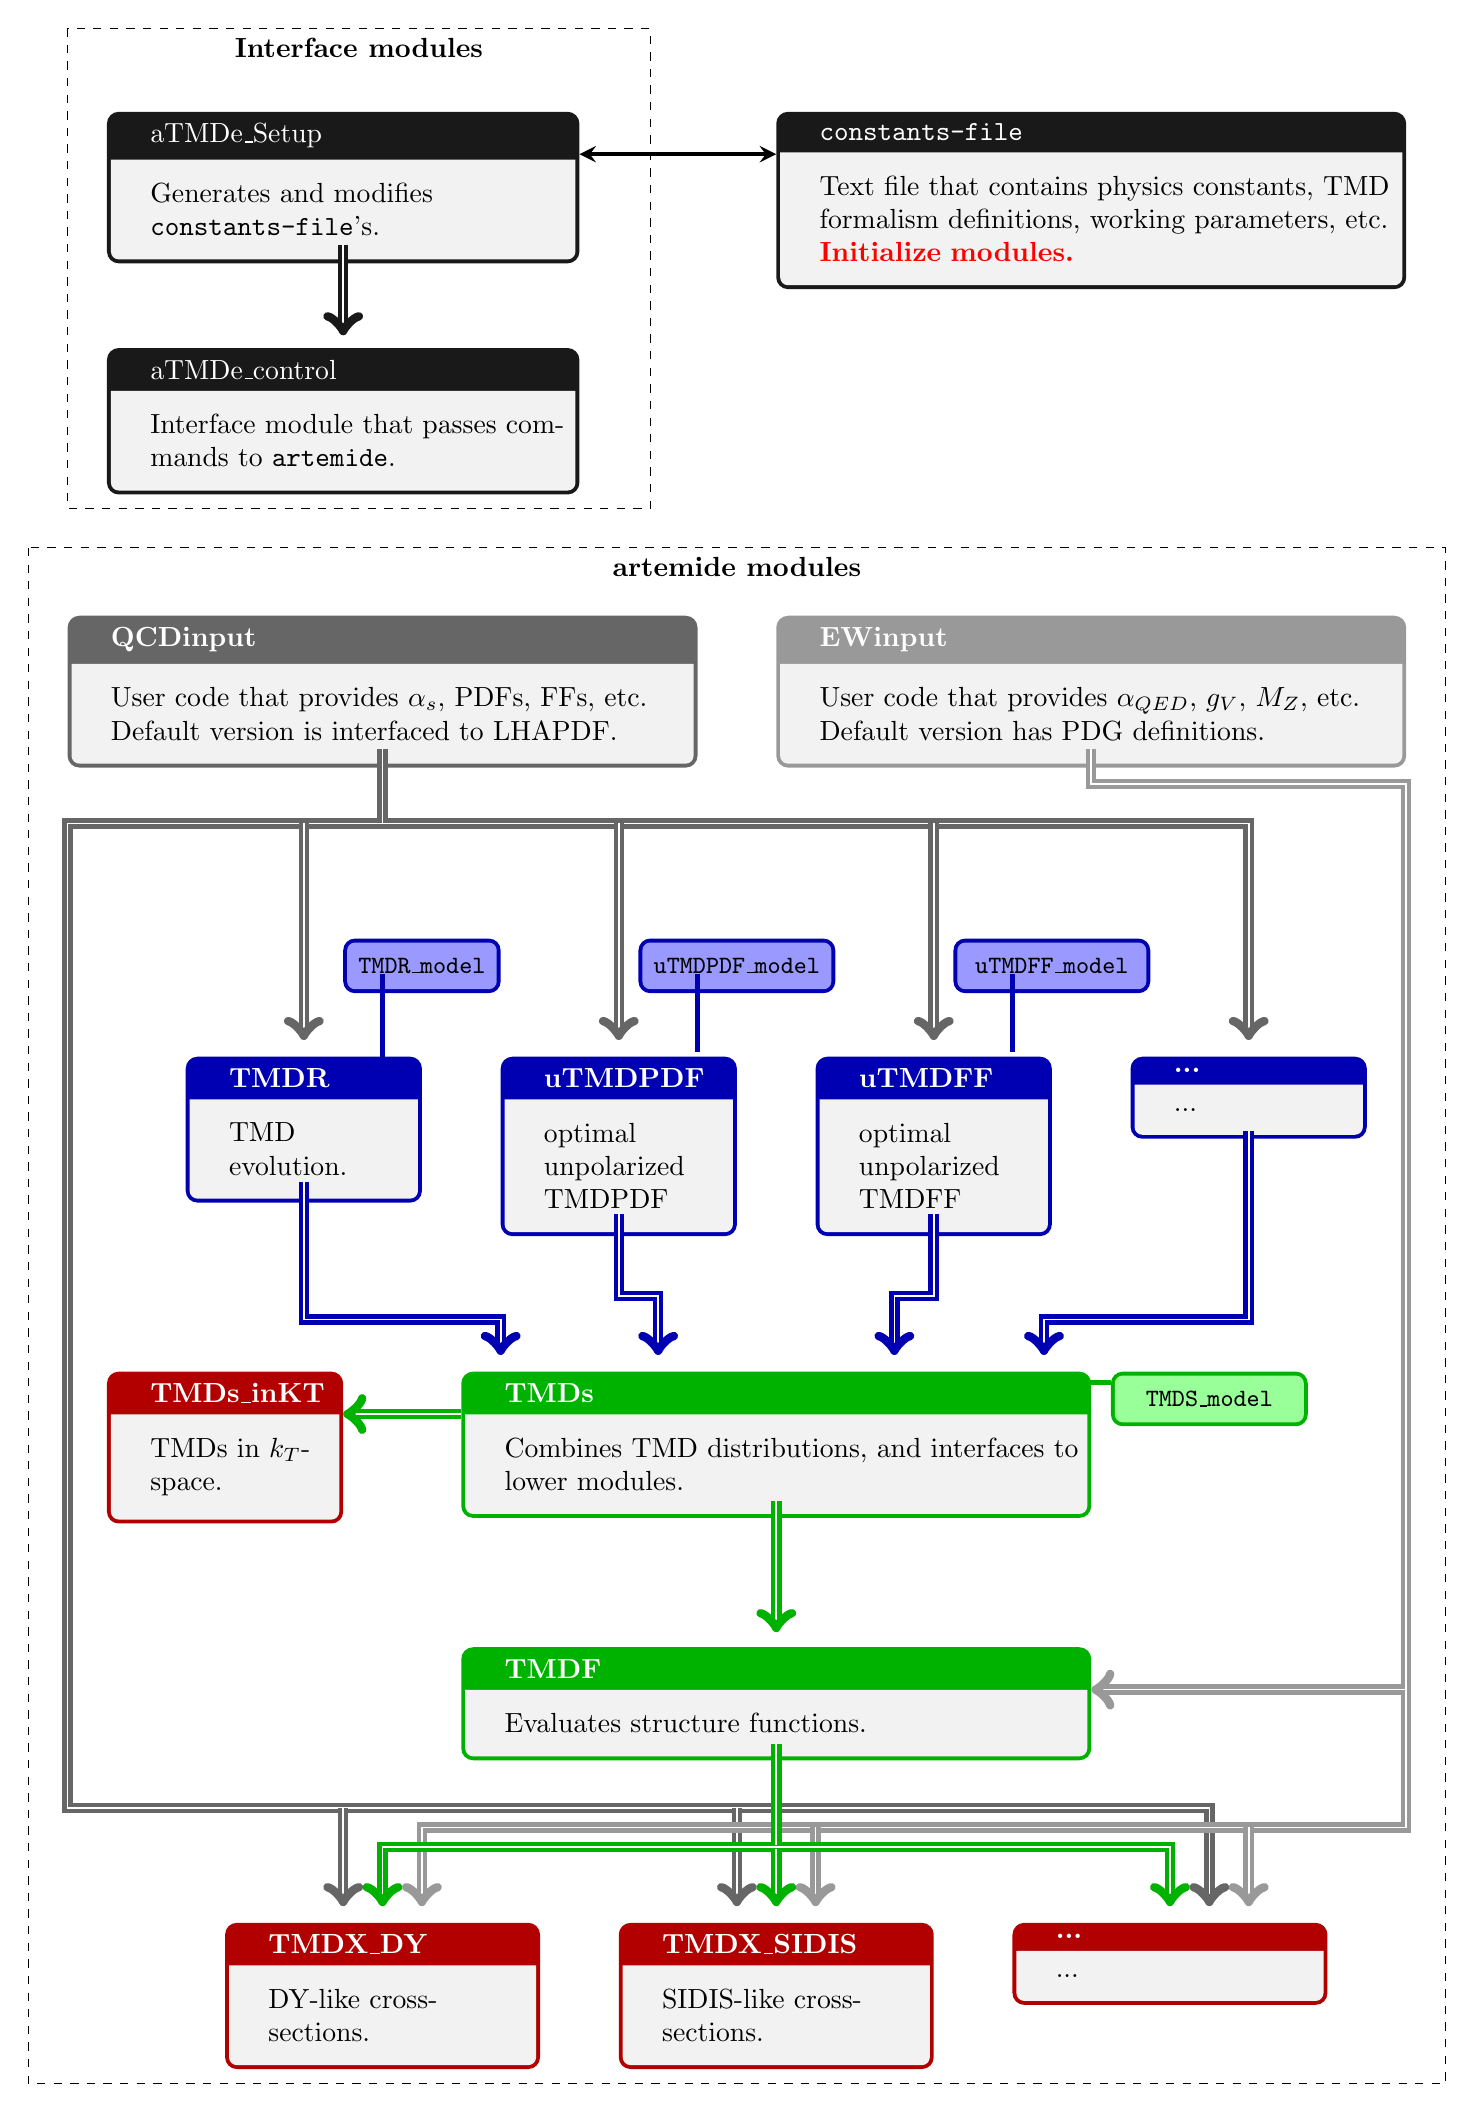
\begin{tikzpicture}

\draw[black,dashed] (-2,16.6) rectangle (5.4,10.5);
\node[below] at (1.7,16.6) {\textbf{Interface modules}};

\node [text width=8cm,below] at (11,16) {
\begin{tcolorbox}[enhanced,title=\texttt{constants-file},colframe=black!90!white,rightupper=0mm]
Text file that contains physics constants, TMD formalism definitions, working parameters, etc.
\\
\red{\textbf{Initialize modules.}}
\end{tcolorbox}};

\node [text width=6cm,below] at (1.5,16) {
\begin{tcolorbox}[enhanced,title=aTMDe\_Setup,colframe=black!90!white,rightupper=0mm]
Generates and modifies \texttt{constants-file}'s.
\end{tcolorbox}};

\node [text width=6cm,below] at (1.5,13) {
\begin{tcolorbox}[enhanced,title=aTMDe\_control,colframe=black!90!white,rightupper=0mm]
Interface module that passes commands to \texttt{artemide}. 
\end{tcolorbox}};

\draw[stealth-stealth,black,ultra thick] (4.5,15)--(7.,15);
\draw[->,white!10!black,ultra thick,double] (1.5,13.85)--(1.5,12.7);
%%%%%%%%%%%%%%%%%%%%%%%%%%%%%%%%%%%%%%%%%%%%%%%%%%%%%%%%%%%%%%%%%%%%%%%%%%%%%%%%%%%%%%%%%%%%%%%%%%%%%%%%%%%%%%%%
\draw[black,dashed] (-2.5,10) rectangle (15.5,-9.5);
\node[below] at (6.5,10) {\textbf{artemide modules}};

\node [text width=8cm,below] at (2,9.6) {
\begin{tcolorbox}[enhanced,title=QCDinput,colframe=black!60!white,fonttitle=\bfseries,
rightupper=0mm]
User code that provides $\alpha_s$, PDFs, FFs, etc.

Default version is interfaced to LHAPDF.
\end{tcolorbox}};

\node [text width=8cm,below] at (11,9.6) {
\begin{tcolorbox}[enhanced,title=EWinput,colframe=black!40!white,fonttitle=\bfseries,
rightupper=0mm]
User code that provides $\alpha_{QED}$, $g_V$, $M_Z$, etc.

Default version has PDG definitions.
\end{tcolorbox}};

\node [text width=3cm,below] at (1,4) {
\begin{tcolorbox}[enhanced,title=TMDR,colframe=blue!70!black,fonttitle=\bfseries,
rightupper=0mm]
TMD \\ evolution.
\end{tcolorbox}};

\node [text width=2cm,below] at (2.5,5.5) {
\begin{tcolorbox}[enhanced,colframe=blue!70!black,fonttitle=\bfseries,
rightupper=0mm,colback=blue!40!white,left=0mm,top=1mm,bottom=1mm]
\center{\small \texttt{TMDR{\_}model}}
\end{tcolorbox}};
\draw[blue!70!black,ultra thick] (2.,4.59)--(2.,3.5);

\node [text width=3cm,below] at (5,4) {
\begin{tcolorbox}[enhanced,title=uTMDPDF,colframe=blue!70!black,fonttitle=\bfseries,
rightupper=0mm]
optimal
\\
unpolarized TMDPDF
\end{tcolorbox}};

\node [text width=2.5cm,below] at (6.5,5.5) {
\begin{tcolorbox}[enhanced,colframe=blue!70!black,fonttitle=\bfseries,
rightupper=0mm,colback=blue!40!white,left=0mm,top=1mm,bottom=1mm]
\center{\small \texttt{uTMDPDF{\_}model}}
\end{tcolorbox}};
\draw[blue!70!black,ultra thick] (6.,4.59)--(6.,3.6);

\node [text width=3cm,below] at (9,4) {
\begin{tcolorbox}[enhanced,title=uTMDFF,colframe=blue!70!black,fonttitle=\bfseries,
rightupper=0mm]
optimal
\\
unpolarized TMDFF
\end{tcolorbox}};

\node [text width=2.5cm,below] at (10.5,5.5) {
\begin{tcolorbox}[enhanced,colframe=blue!70!black,fonttitle=\bfseries,
rightupper=0mm,colback=blue!40!white,left=0mm,top=1mm,bottom=1mm]
\center{\small \texttt{uTMDFF{\_}model}}
\end{tcolorbox}};
\draw[blue!70!black,ultra thick] (10.,4.59)--(10.,3.6);

\node [text width=3cm,below] at (13,4) {
\begin{tcolorbox}[enhanced,title=...,colframe=blue!70!black,fonttitle=\bfseries,
rightupper=0mm]
...
\end{tcolorbox}};


\draw[<->,black!60!white,ultra thick,double] (12.5,-7.25)--(12.5,-6)--(-2,-6)--(-2,6.5) -- (13,6.5) -- (13,3.75);
\draw[->,black!60!white,ultra thick,double] (6.5,-6)--(6.5,-7.25);
\draw[->,black!60!white,ultra thick,double] (1.5,-6)--(1.5,-7.25);
\draw[black!60!white,ultra thick,double] (2,7.45) -- (2,6.5);
\draw[->,black!60!white,ultra thick,double] (9,6.5) -- (9,3.75);
\draw[->,black!60!white,ultra thick,double] (5,6.5) -- (5,3.75);
\draw[->,black!60!white,ultra thick,double] (1,6.5) -- (1,3.75);

\draw[->,black!40!white,ultra thick,double] (11,7.45)--(11,7.0)--(15,7.0)--(15,-4.5)--(11,-4.5);
\draw[->,black!40!white,ultra thick,double] (15,-4.5)--(15,-6.25)--(2.5,-6.25)--(2.5,-7.25);
\draw[->,black!40!white,ultra thick,double] (7.5,-6.25)--(7.5,-7.25);
\draw[->,black!40!white,ultra thick,double] (13,-6.25)--(13,-7.25);

\node [text width=8cm,below] at (7,0) {
\begin{tcolorbox}[enhanced,title=TMDs,colframe=green!70!black,fonttitle=\bfseries,
rightupper=0mm]
Combines TMD distributions, and interfaces to lower modules.
\end{tcolorbox}};

\draw[->,green!70!black,ultra thick,double] (3,-1) -- (1.5,-1);
\node [text width=3cm,below] at (0,0) {
\begin{tcolorbox}[enhanced,title=TMDs\_inKT,colframe=red!70!black,fonttitle=\bfseries,
rightupper=0mm]
TMDs in $k_T$-space.
\end{tcolorbox}};

\node [text width=2.5cm,below] at (12.5,0) {
\begin{tcolorbox}[enhanced,colframe=green!70!black,fonttitle=\bfseries,
rightupper=0mm,colback=green!40!white,left=0mm,top=1mm,bottom=1mm]
\center{\small \texttt{TMDS{\_}model}}
\end{tcolorbox}};
\draw[green!70!black,ultra thick] (10.,-0.6)--(11.25,-0.6);

\draw[->,blue!70!black,ultra thick,double] (1,1.95) -- (1,0.2)-- (3.5,0.2)-- (3.5,-0.25);
\draw[->,blue!70!black,ultra thick,double] (5,1.54) -- (5,0.5)-- (5.5,0.5)-- (5.5,-0.25);
\draw[->,blue!70!black,ultra thick,double] (9,1.54) -- (9,0.5)-- (8.5,0.5)-- (8.5,-0.25);
\draw[->,blue!70!black,ultra thick,double] (13,2.6) -- (13,0.2)-- (10.4,0.2)-- (10.4,-0.25);

\node [text width=8cm,below] at (7,-3.5) {
\begin{tcolorbox}[enhanced,title=TMDF,colframe=green!70!black,fonttitle=\bfseries,
rightupper=0mm]
Evaluates structure functions.
\end{tcolorbox}};

\draw[->,green!70!black,ultra thick,double] (7,-2.1) -- (7,-3.77);

\node [text width=4cm,below] at (2,-7) {
\begin{tcolorbox}[enhanced,title=TMDX{\_}DY,colframe=red!70!black,fonttitle=\bfseries,
rightupper=0mm]
DY-like cross-sections.
\end{tcolorbox}};

\node [text width=4cm,below] at (7,-7) {
\begin{tcolorbox}[enhanced,title=TMDX{\_}SIDIS,colframe=red!70!black,fonttitle=\bfseries,
rightupper=0mm]
SIDIS-like cross-sections.
\end{tcolorbox}};

\node [text width=4cm,below] at (12,-7) {
\begin{tcolorbox}[enhanced,title=...,colframe=red!70!black,fonttitle=\bfseries,
rightupper=0mm]
...
\end{tcolorbox}};

\draw[<->,green!70!black,ultra thick,double] (2,-7.25) -- (2,-6.5) -- (12,-6.5) -- (12,-7.25);
\draw[green!70!black,ultra thick,double] (7,-6.47) -- (7,-5.19);
\draw[->,green!70!black,ultra thick,double] (7,-6.52) -- (7,-7.25);

\end{tikzpicture}
}
\end{center}

\newpage

\subsection{artemide structure before v2.00}

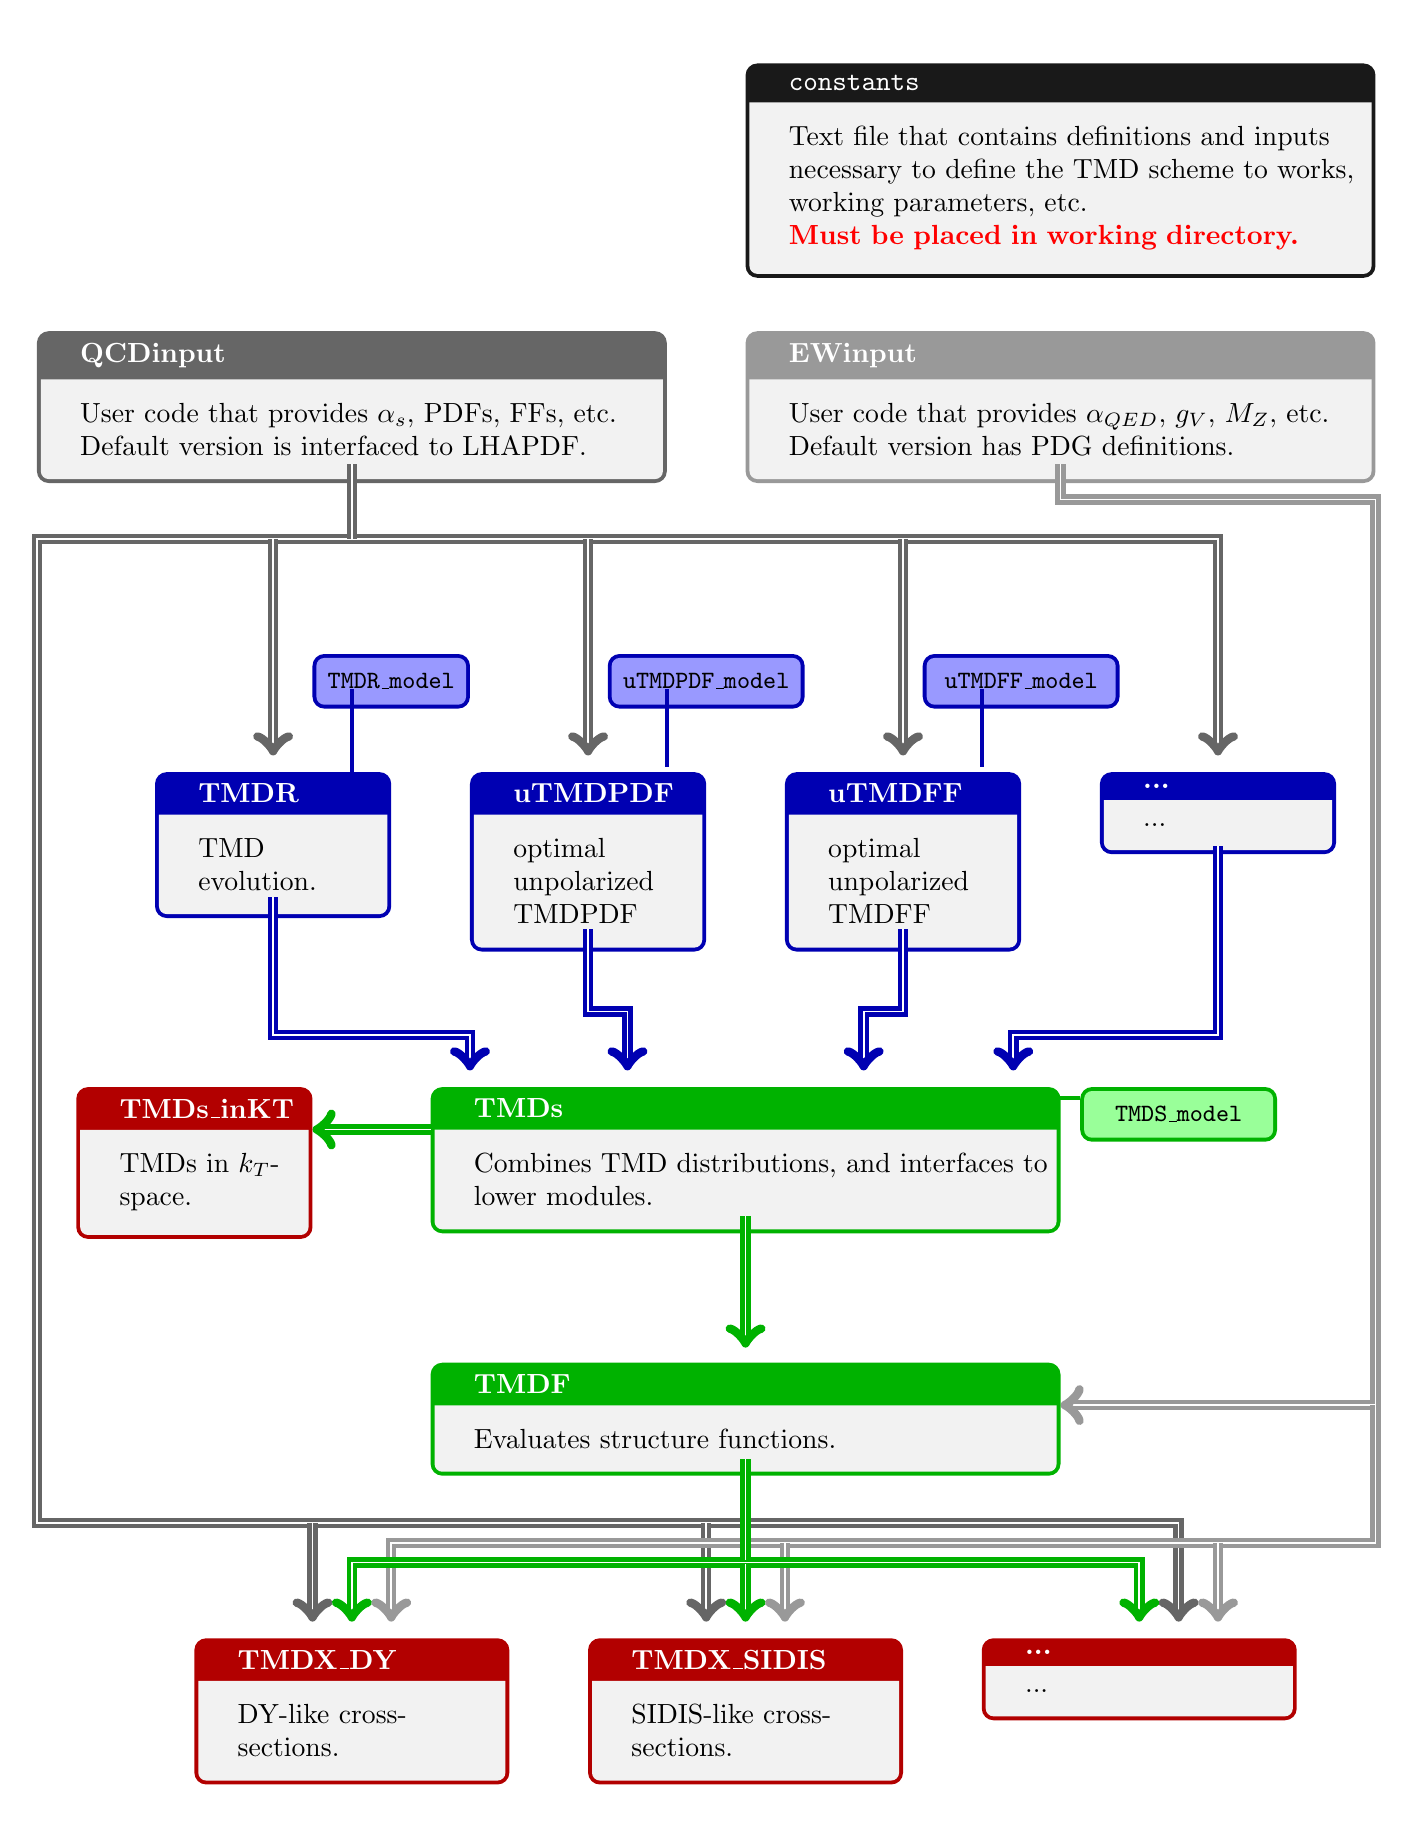
\begin{tikzpicture}
\node [text width=8cm,below] at (2,9.6) {
\begin{tcolorbox}[enhanced,title=QCDinput,colframe=black!60!white,fonttitle=\bfseries,
rightupper=0mm]
User code that provides $\alpha_s$, PDFs, FFs, etc.

Default version is interfaced to LHAPDF.
\end{tcolorbox}};

\node [text width=8cm,below] at (11,9.6) {
\begin{tcolorbox}[enhanced,title=EWinput,colframe=black!40!white,fonttitle=\bfseries,
rightupper=0mm]
User code that provides $\alpha_{QED}$, $g_V$, $M_Z$, etc.

Default version has PDG definitions.
\end{tcolorbox}};

\node [text width=8cm,below] at (11,13) {
\begin{tcolorbox}[enhanced,title=\texttt{constants},colframe=black!90!white,rightupper=0mm]
Text file that contains definitions and inputs necessary to define the TMD scheme to works, working parameters, etc.
\\
\red{\textbf{Must be placed in working directory.}}
\end{tcolorbox}};


\node [text width=3cm,below] at (1,4) {
\begin{tcolorbox}[enhanced,title=TMDR,colframe=blue!70!black,fonttitle=\bfseries,
rightupper=0mm]
TMD \\ evolution.
\end{tcolorbox}};

\node [text width=2cm,below] at (2.5,5.5) {
\begin{tcolorbox}[enhanced,colframe=blue!70!black,fonttitle=\bfseries,
rightupper=0mm,colback=blue!40!white,left=0mm,top=1mm,bottom=1mm]
\center{\small \texttt{TMDR{\_}model}}
\end{tcolorbox}};
\draw[blue!70!black,ultra thick] (2.,4.59)--(2.,3.5);

\node [text width=3cm,below] at (5,4) {
\begin{tcolorbox}[enhanced,title=uTMDPDF,colframe=blue!70!black,fonttitle=\bfseries,
rightupper=0mm]
optimal
\\
unpolarized TMDPDF
\end{tcolorbox}};

\node [text width=2.5cm,below] at (6.5,5.5) {
\begin{tcolorbox}[enhanced,colframe=blue!70!black,fonttitle=\bfseries,
rightupper=0mm,colback=blue!40!white,left=0mm,top=1mm,bottom=1mm]
\center{\small \texttt{uTMDPDF{\_}model}}
\end{tcolorbox}};
\draw[blue!70!black,ultra thick] (6.,4.59)--(6.,3.6);

\node [text width=3cm,below] at (9,4) {
\begin{tcolorbox}[enhanced,title=uTMDFF,colframe=blue!70!black,fonttitle=\bfseries,
rightupper=0mm]
optimal
\\
unpolarized TMDFF
\end{tcolorbox}};

\node [text width=2.5cm,below] at (10.5,5.5) {
\begin{tcolorbox}[enhanced,colframe=blue!70!black,fonttitle=\bfseries,
rightupper=0mm,colback=blue!40!white,left=0mm,top=1mm,bottom=1mm]
\center{\small \texttt{uTMDFF{\_}model}}
\end{tcolorbox}};
\draw[blue!70!black,ultra thick] (10.,4.59)--(10.,3.6);

\node [text width=3cm,below] at (13,4) {
\begin{tcolorbox}[enhanced,title=...,colframe=blue!70!black,fonttitle=\bfseries,
rightupper=0mm]
...
\end{tcolorbox}};


\draw[<->,black!60!white,ultra thick,double] (12.5,-7.25)--(12.5,-6)--(-2,-6)--(-2,6.5) -- (13,6.5) -- (13,3.75);
\draw[->,black!60!white,ultra thick,double] (6.5,-6)--(6.5,-7.25);
\draw[->,black!60!white,ultra thick,double] (1.5,-6)--(1.5,-7.25);
\draw[black!60!white,ultra thick,double] (2,7.45) -- (2,6.5);
\draw[->,black!60!white,ultra thick,double] (9,6.5) -- (9,3.75);
\draw[->,black!60!white,ultra thick,double] (5,6.5) -- (5,3.75);
\draw[->,black!60!white,ultra thick,double] (1,6.5) -- (1,3.75);

\draw[->,black!40!white,ultra thick,double] (11,7.45)--(11,7.0)--(15,7.0)--(15,-4.5)--(11,-4.5);
\draw[->,black!40!white,ultra thick,double] (15,-4.5)--(15,-6.25)--(2.5,-6.25)--(2.5,-7.25);
\draw[->,black!40!white,ultra thick,double] (7.5,-6.25)--(7.5,-7.25);
\draw[->,black!40!white,ultra thick,double] (13,-6.25)--(13,-7.25);

\node [text width=8cm,below] at (7,0) {
\begin{tcolorbox}[enhanced,title=TMDs,colframe=green!70!black,fonttitle=\bfseries,
rightupper=0mm]
Combines TMD distributions, and interfaces to lower modules.
\end{tcolorbox}};

\draw[->,green!70!black,ultra thick,double] (3,-1) -- (1.5,-1);
\node [text width=3cm,below] at (0,0) {
\begin{tcolorbox}[enhanced,title=TMDs\_inKT,colframe=red!70!black,fonttitle=\bfseries,
rightupper=0mm]
TMDs in $k_T$-space.
\end{tcolorbox}};

\node [text width=2.5cm,below] at (12.5,0) {
\begin{tcolorbox}[enhanced,colframe=green!70!black,fonttitle=\bfseries,
rightupper=0mm,colback=green!40!white,left=0mm,top=1mm,bottom=1mm]
\center{\small \texttt{TMDS{\_}model}}
\end{tcolorbox}};
\draw[green!70!black,ultra thick] (10.,-0.6)--(11.25,-0.6);

\draw[->,blue!70!black,ultra thick,double] (1,1.95) -- (1,0.2)-- (3.5,0.2)-- (3.5,-0.25);
\draw[->,blue!70!black,ultra thick,double] (5,1.54) -- (5,0.5)-- (5.5,0.5)-- (5.5,-0.25);
\draw[->,blue!70!black,ultra thick,double] (9,1.54) -- (9,0.5)-- (8.5,0.5)-- (8.5,-0.25);
\draw[->,blue!70!black,ultra thick,double] (13,2.6) -- (13,0.2)-- (10.4,0.2)-- (10.4,-0.25);

\node [text width=8cm,below] at (7,-3.5) {
\begin{tcolorbox}[enhanced,title=TMDF,colframe=green!70!black,fonttitle=\bfseries,
rightupper=0mm]
Evaluates structure functions.
\end{tcolorbox}};

\draw[->,green!70!black,ultra thick,double] (7,-2.1) -- (7,-3.77);

\node [text width=4cm,below] at (2,-7) {
\begin{tcolorbox}[enhanced,title=TMDX{\_}DY,colframe=red!70!black,fonttitle=\bfseries,
rightupper=0mm]
DY-like cross-sections.
\end{tcolorbox}};

\node [text width=4cm,below] at (7,-7) {
\begin{tcolorbox}[enhanced,title=TMDX{\_}SIDIS,colframe=red!70!black,fonttitle=\bfseries,
rightupper=0mm]
SIDIS-like cross-sections.
\end{tcolorbox}};

\node [text width=4cm,below] at (12,-7) {
\begin{tcolorbox}[enhanced,title=...,colframe=red!70!black,fonttitle=\bfseries,
rightupper=0mm]
...
\end{tcolorbox}};

\draw[<->,green!70!black,ultra thick,double] (2,-7.25) -- (2,-6.5) -- (12,-6.5) -- (12,-7.25);
\draw[green!70!black,ultra thick,double] (7,-6.47) -- (7,-5.19);
\draw[->,green!70!black,ultra thick,double] (7,-6.52) -- (7,-7.25);

\end{tikzpicture}

\newpage

\subsection{artemide structure before v1.3}

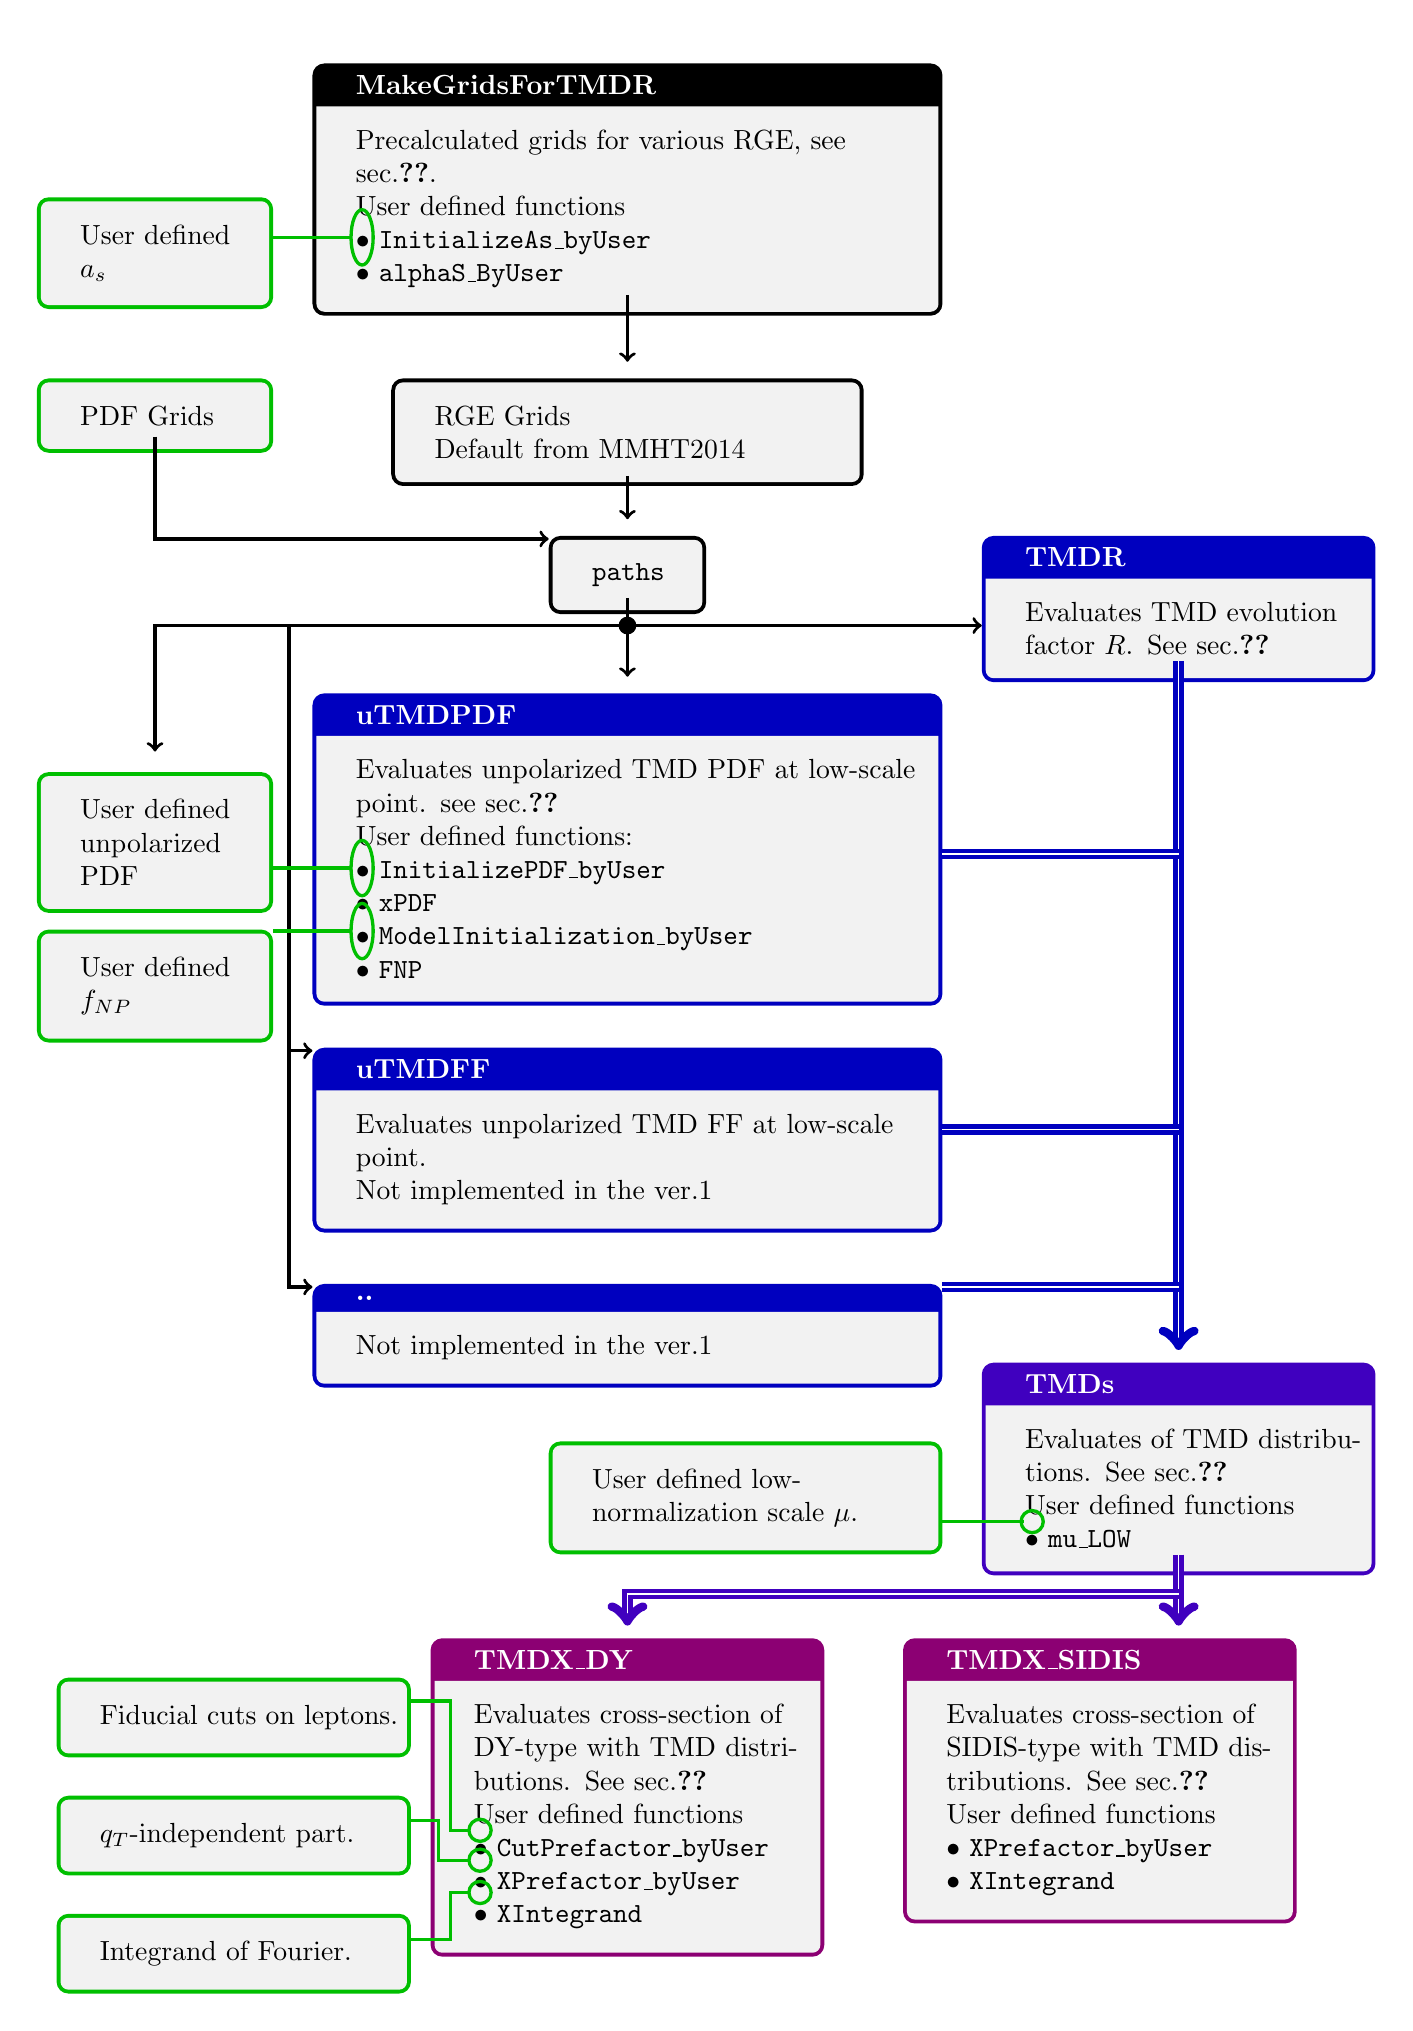
\begin{tikzpicture}
\node [text width=8cm,below] at (6,8) {
\begin{tcolorbox}[enhanced,title=MakeGridsForTMDR,colframe=black,fonttitle=\bfseries,
rightupper=0mm]
Precalculated grids for various RGE, see sec.\ref{sec:grids_TMDR}.
\\
User defined functions
\\$\bullet$ \texttt{InitializeAs{\_}byUser}
\\$\bullet$ \texttt{alphaS{\_}ByUser}
\end{tcolorbox}};
\node [text width=3cm,below] at (0,6.3) {
\begin{tcolorbox}[enhanced,colframe=green!75!black,rightupper=0mm]
User defined $a_s$
\end{tcolorbox}};
\draw[green!75!black,very thick] (1.5,5.33) -- (2.5,5.33);
\draw[green!75!black,very thick] (2.63,5.33) ellipse (4pt and 10pt);


\node [text width=6cm,below] at (6,4) {
\begin{tcolorbox}[enhanced,colframe=black,rightupper=0mm]
RGE Grids
\\
Default from MMHT2014
\end{tcolorbox}};
\node [text width=3cm,below] at (0,4) {
\begin{tcolorbox}[enhanced,colframe=green!75!black,rightupper=0mm]
PDF Grids
\end{tcolorbox}};
\draw[->,black,very thick] (6,4.6) -- (6,3.75);

\node [text width=2cm,below] at (6,2) {
\begin{tcolorbox}[enhanced,colframe=black,rightupper=0mm]
\texttt{paths}
\end{tcolorbox}};
\draw[->,black,very thick] (6,2.3) -- (6,1.75);
\draw[->,black,very thick] (0,2.8) -- (0,1.5) -- (5,1.5);
\draw[black,very thick] (6,0.75) -- (6,0.4);
\draw[fill=black] (6,0.4) circle (3pt);
\draw[->,black,very thick] (6,0.4) -- (0,0.4) -- (0,-1.2);
\draw[->,black,very thick] (6,0.4) -- (10.5,0.4);
\draw[->,black,very thick] (6,0.4) -- (6,-0.25);
\draw[->,black,very thick] (1.7,0.4) -- (1.7,-5) -- (2,-5);
\draw[->,black,very thick] (1.7,0.4) -- (1.7,-8) -- (2,-8);

\node [text width=8cm,below] at (6,0) {
\begin{tcolorbox}[enhanced,title=uTMDPDF,colframe=blue!75!black,fonttitle=\bfseries,
rightupper=0mm]
Evaluates unpolarized TMD PDF at low-scale point.
see sec.\ref{uTMDPDF}
\\ User defined functions:
\\$\bullet$ \texttt{InitializePDF{\_}byUser}
\\$\bullet$ \texttt{xPDF}
\\$\bullet$ \texttt{ModelInitialization{\_}byUser}
\\$\bullet$ \texttt{FNP}
\end{tcolorbox}};

\node [text width=5cm,below] at (13,2) {
\begin{tcolorbox}[enhanced,title=TMDR,colframe=blue!75!black,fonttitle=\bfseries,
rightupper=0mm]
Evaluates TMD evolution factor $R$.
See sec.\ref{TMDR}
\end{tcolorbox}};

\node [text width=3cm,below] at (0,-1.) {
\begin{tcolorbox}[enhanced,colframe=green!75!black,rightupper=0mm]
User defined unpolarized PDF
\end{tcolorbox}};
\draw[green!75!black,very thick] (1.5,-2.68) -- (2.5,-2.68);
\draw[green!75!black,very thick] (2.63,-2.68) ellipse (4pt and 10pt);

\node [text width=3cm,below] at (0,-3) {
\begin{tcolorbox}[enhanced,colframe=green!75!black,rightupper=0mm]
User defined $f_{NP}$
\end{tcolorbox}};
\draw[green!75!black,very thick] (1.5,-3.48) -- (2.5,-3.48);
\draw[green!75!black,very thick] (2.63,-3.48) ellipse (4pt and 10pt);


\node [text width=8cm,below] at (6,-4.5) {
\begin{tcolorbox}[enhanced,title=uTMDFF,colframe=blue!75!black,fonttitle=\bfseries,
rightupper=0mm]
Evaluates unpolarized TMD FF at low-scale point.
\\
Not implemented in the ver.1
\end{tcolorbox}};

\node [text width=8cm,below] at (6,-7.5) {
\begin{tcolorbox}[enhanced,title=..,colframe=blue!75!black,fonttitle=\bfseries,
rightupper=0mm]
Not implemented in the ver.1
\end{tcolorbox}};


\node [text width=5cm,below] at (13,-8.5) {
\begin{tcolorbox}[enhanced,title=TMDs,colframe=blue!75!red,fonttitle=\bfseries,
rightupper=0mm]
Evaluates of TMD distributions. See sec.\ref{TMDs}
\\
User defined functions
\\$\bullet$ \texttt{mu{\_}LOW}
\end{tcolorbox}};
\draw[->,blue!75!black,ultra thick,double] (13,-0.05) -- (13,-8.8);
\draw[blue!75!black,ultra thick,double] (10,-2.5) -- (13,-2.5);
\draw[blue!75!black,ultra thick,double] (10,-6) -- (13,-6);
\draw[blue!75!black,ultra thick,double] (10,-8) -- (13,-8);

\node [text width=5cm,below] at (7.5,-9.5) {
\begin{tcolorbox}[enhanced,colframe=green!75!black,rightupper=0mm]
User defined low-normalization scale $\mu$.
\end{tcolorbox}};
\draw[green!75!black,very thick] (10,-10.98) -- (11.03,-10.98);
\draw[green!75!black,very thick] (11.14,-10.98) ellipse (4pt and 4pt);

\node [text width=5cm,below] at (6,-12) {
\begin{tcolorbox}[enhanced,title=TMDX\_DY,colframe=blue!45!red,fonttitle=\bfseries,
rightupper=0mm]
Evaluates cross-section of DY-type with TMD distributions. See sec.\ref{TMDX}
\\
User defined functions
\\$\bullet$ \texttt{CutPrefactor{\_}byUser}
\\$\bullet$ \texttt{XPrefactor{\_}byUser}
\\$\bullet$ \texttt{XIntegrand}
\end{tcolorbox}};
\draw[->,blue!75!red,ultra thick,double] (13,-11.4) -- (13,-12.3);

\node [text width=4.5cm,below] at (1,-12.5) {
\begin{tcolorbox}[enhanced,colframe=green!75!black,rightupper=0mm]
Fiducial cuts on leptons.
\end{tcolorbox}};
\node [text width=4.5cm,below] at (1,-14) {
\begin{tcolorbox}[enhanced,colframe=green!75!black,rightupper=0mm]
$q_T$-independent part.
\end{tcolorbox}};
\node [text width=4.5cm,below] at (1,-15.5) {
\begin{tcolorbox}[enhanced,colframe=green!75!black,rightupper=0mm]
Integrand of Fourier.
\end{tcolorbox}};
\draw[green!75!black,very thick] (4.128,-14.9) ellipse (4pt and 4pt);
\draw[green!75!black,very thick] (4.128,-15.28) ellipse (4pt and 4pt);
\draw[green!75!black,very thick] (4.128,-15.69) ellipse (4pt and 4pt);

\draw[green!75!black,very thick] (3.25,-13.26) -- (3.75,-13.26) -- (3.75,-14.9) -- (4,-14.9);
\draw[green!75!black,very thick] (3.25,-14.78) -- (3.6,-14.78) -- (3.6,-15.28) -- (4,-15.28);
\draw[green!75!black,very thick] (3.25,-16.29) -- (3.75,-16.29) -- (3.75,-15.69) -- (4,-15.69);


\node [text width=5cm,below] at (12,-12) {
\begin{tcolorbox}[enhanced,title=TMDX\_SIDIS,colframe=blue!45!red,fonttitle=\bfseries,
rightupper=0mm]
Evaluates cross-section of SIDIS-type with TMD distributions. See sec.\ref{TMDX}
\\
User defined functions
\\$\bullet$ \texttt{XPrefactor{\_}byUser}
\\$\bullet$ \texttt{XIntegrand}
\end{tcolorbox}};

\draw[->,blue!75!red,ultra thick,double] (13,-11.9) -- (6,-11.9) -- (6,-12.3);

\end{tikzpicture}

\end{document}

# added by Anaconda2 2018.12 installer
# >>> conda init >>>
# !! Contents within this block are managed by 'conda init' !!
__conda_setup="$(CONDA_REPORT_ERRORS=false '/home/vla18041/LinkData2/anaconda2/bin/conda' shell.bash hook 2> /dev/null)"
if [ $? -eq 0 ]; then
    \eval "$__conda_setup"
else
    if [ -f "/home/vla18041/LinkData2/anaconda2/etc/profile.d/conda.sh" ]; then
        . "/home/vla18041/LinkData2/anaconda2/etc/profile.d/conda.sh"
        CONDA_CHANGEPS1=false conda activate base
    else
        \export PATH="/home/vla18041/LinkData2/anaconda2/bin:$PATH"
    fi
fi
unset __conda_setup
# <<< conda init <<<